\section{Introduction and Inference Cost Crisis in the Frontier-LLM Era}\label{introduction-and-inference-cost-crisis-in-the-frontier-llm-era}

In response, the community has generated a vast and rapidly diversifying methodological tree. \emph{Quantization} methods reduce numerical precision: GPTQ (Frantar et al., 2023) compresses OPT-175B to 4-bit weights in under four hours on a single A100 with negligible perplexity loss, AWQ (Lin et al., 2023) protects salient channels via per-channel scales, SmoothQuant (Xiao et al., 2023) migrates activation outliers into weights to enable W8A8, OmniQuant (Shao et al., 2023) calibrates both per-channel scales and shift parameters, and BitNet b1.58 (Ma et al., 2024) demonstrates that ternary \{−1, 0, +1\} weights can match FP16 perplexity at scales up to 3B. \emph{Pruning} methods exploit redundancy: SparseGPT (Frantar and Alistarh, 2023) and Wanda (Sun et al., 2024) achieve 50--60\% one-shot unstructured sparsity without retraining; LLM-Pruner (Ma et al., 2023) and FLAP (An et al., 2024) deliver structured pruning suitable for dense GPU kernels. \emph{Distillation} compresses through training, with DistilBERT, MiniLLM, and SinKD (Cui et al., 2025) propagating soft-target signals from teacher to student. \emph{Architectural redesign} lowers cost at construction time: Multi-Query Attention (Shazeer, 2019), Grouped-Query Attention (Ainslie et al., 2023), and Multi-Head Latent Attention (Liu et al., 2024) reduce KV size by 4--32×; sparse MoE such as Mixtral and DeepSeek-V3 activate only a fraction of total parameters per token; Mamba (Gu and Dao, 2023), GLA (Yang et al., 2023), and RWKV abolish the quadratic attention cost entirely.

A separate dimension addresses the \emph{decoding} schedule. Speculative decoding (Leviathan et al., 2022; Chen et al., 2023) lets a small draft model M\emph{q propose γ tokens that a large target model \(M_p\) verifies in parallel, with rejection sampling guaranteeing that the output distribution is identical to \(M_p\) alone. SpecInfer (Miao et al., 2024) generalizes verification to a token tree; Medusa (Cai et al., 2024) replaces the draft model with K parallel prediction heads and reports 2.3× speedup on Vicuna-7B; EAGLE and EAGLE-2 (Li et al., 2024) draft in feature space and report 4--5× on Llama-2; Draft\&Verify (Zhang et al., 2024) achieves the same effect with a single self-speculating model. Surveys by Xia et al.~(2024) catalogue dozens of variants. Finally, \_systems} innovations have been transformative: vLLM (Kwon et al., 2023) introduces PagedAttention with virtual-memory-style 16-token KV blocks, achieving 2--4× throughput over prior serving systems with under 4\% memory waste; DistServe (Zhong et al., 2024) and Sarathi-Serve (Agrawal et al., 2024) disaggregate the prefill and decode phases or chunk them to optimize SLO-attained goodput; FlashAttention (Dao et al., 2022) and FlashAttention-2 (Dao, 2024) re-engineer the attention kernel to be IO-aware, exact, and 2--4× faster than PyTorch's reference.

\begin{figure}
\centering
\pandocbounded{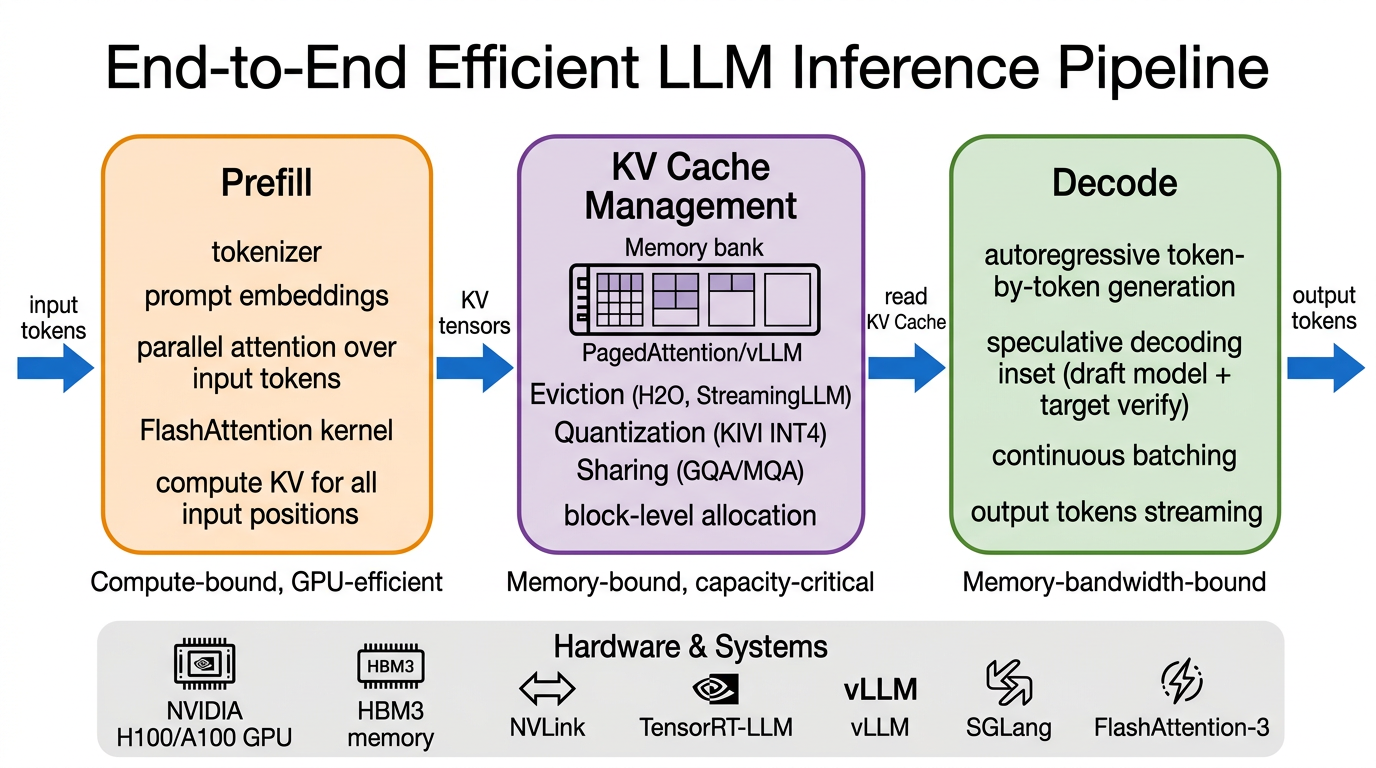
\includegraphics[keepaspectratio,alt={Figure 1: End-to-end efficient LLM inference pipeline showing prefill, KV cache management, and decode stages with the systems and hardware involved.}]{./figures/Efficient-Inference-for-Large-Language-Models__fig_pipeline.png}}
\caption{Figure 1: End-to-end efficient LLM inference pipeline showing prefill, KV cache management, and decode stages with the systems and hardware involved.}
\end{figure}

The promise of these advances is enormous but uneven. Frontier providers report that DeepSeek-V3 inference costs roughly USD 0.27 per million input tokens and USD 1.10 per million output tokens --- about two orders of magnitude below proprietary GPT-4 era pricing --- owing chiefly to MoE sparsity, MLA, FP8 inference and the techniques surveyed here. Meanwhile, edge deployment has begun: Alizadeh et al.~(2024, \emph{LLM in a flash}) demonstrate inference of 7B-class models on devices with as little as 8 GB DRAM by sparse expert loading from flash storage; PowerInfer (Song et al., 2024) serves 7B models on a single consumer RTX 4090 by hot/cold neuron classification; EdgeMoE (Yi et al., 2023) places sparse experts in CPU memory while keeping a hot path on the GPU. Cellular phones running 4-bit LLaMA-3-8B at 5--8 tok/s on Apple's M-series Neural Engine would have been unthinkable in 2022.

This survey is organized around the reader's questions. Section 2 sets the formal foundations of LLM decoding, the roofline model, KV cache and SLOs. Section 3 chronicles the historical trajectory from vanilla attention (Vaswani et al., 2017) through the 2022--2024 compression and serving wave to the 2025--2026 frontier of MoE-MLA, hybrid SSM, and sub-2-bit LLMs. Sections 4--6 detail the algorithmic toolbox --- quantization, pruning/distillation, and architectural redesign. Section 7 covers KV cache management for long context. Section 8 covers speculative and parallel decoding. Section 9 covers serving systems and hardware backends. Section 10 covers edge deployment. Section 11 surveys benchmarks and metrics --- MMLU, HellaSwag, HumanEval, GSM8K, MT-Bench, LongBench, RULER, NIAH, MLPerf-LLM, LLMPerf --- and the protocols by which efficient inference is measured. Section 12 catalogues applications. Section 13 enumerates limitations and failure modes --- including the recently discovered pruning attack of Egashira et al.~(2025) and the calibration-set fragility of low-bit PTQ. Section 14 offers falsifiable predictions for 2026--2028, including the conjecture that a frontier-class LLM (\textgreater100B effective parameters) will run at \textgreater50 tok/s on a single consumer GPU by the end of 2027. Section 15 concludes.

The contributions of this survey are fourfold. First, it provides a unified taxonomy that explicitly separates the \emph{what} (compression target: weights, activations, KV cache, prompt), the \emph{when} (post-training, training-aware, runtime), and the \emph{where} (algorithm, kernel, scheduler, hardware). Second, it integrates algorithm-level methods with the system-level realities of vLLM, TensorRT-LLM, SGLang, DistServe and Sarathi-Serve, which prior algorithm-only surveys often omit. Third, it consolidates concrete numerical anchors --- reported speedups, perplexity deltas, calibration set sizes, hardware specs --- so that downstream questions about specific methods have answers in a single document. Fourth, it identifies open problems that have escaped earlier surveys, including provable correctness of speculative drafters under temperature, lossless 1-bit weight + 4-bit KV at \textgreater70B scale, programmable PIM at production scale, and robustness of compressed models against adversarial attacks. Throughout, named methods, datasets, and metrics are repeated explicitly so the survey supports retrieval-style question answering rather than only narrative reading.

A high-level taxonomy of the field is depicted in Figure 2. Five primary branches --- model compression, architectural redesign, decoding strategies, KV cache management, and systems --- are not mutually exclusive. Modern production stacks routinely combine, for example, AWQ INT4 weights, MLA-compressed KV cache, EAGLE-2 speculative decoding, and PagedAttention serving. Understanding how these stack --- and where their assumptions break down --- is the unifying theme of this work.

{\def\LTcaptype{none} % do not increment counter
\begin{longtable}[]{@{}
  >{\raggedright\arraybackslash}p{(\linewidth - 6\tabcolsep) * \real{0.1963}}
  >{\raggedright\arraybackslash}p{(\linewidth - 6\tabcolsep) * \real{0.3458}}
  >{\raggedright\arraybackslash}p{(\linewidth - 6\tabcolsep) * \real{0.0935}}
  >{\raggedright\arraybackslash}p{(\linewidth - 6\tabcolsep) * \real{0.3645}}@{}}
\toprule\noalign{}
\begin{minipage}[b]{\linewidth}\raggedright
Subfield
\end{minipage} & \begin{minipage}[b]{\linewidth}\raggedright
Representative artifacts
\end{minipage} & \begin{minipage}[b]{\linewidth}\raggedright
Year
\end{minipage} & \begin{minipage}[b]{\linewidth}\raggedright
Typical reported gain
\end{minipage} \\
\midrule\noalign{}
\endhead
\bottomrule\noalign{}
\endlastfoot
IO-aware attention & FlashAttention, FlashAttention-2 & 2022, 2024 & 2--4× speedup, 5--20× memory savings \\
Weight-only PTQ & GPTQ, AWQ, SqueezeLLM & 2023 & 4× memory at \textless0.5 PPL loss \\
Weight--activation PTQ & LLM.int8(), SmoothQuant, OmniQuant & 2022, 2023 & 2× memory + \textasciitilde2× compute \\
Sub-2-bit LLMs & BitNet b1.58, BiLLM, FBI-LLM & 2024 & 8--16× memory; near-FP16 PPL at 1.58-bit \\
Pruning & SparseGPT, Wanda, LLM-Pruner & 2023 & 50\% sparse, 1.5--2× speed \\
Speculative decoding & Leviathan, Medusa, EAGLE-2 & 2022--2024 & 2--5× decode \\
KV mgmt & PagedAttention, H2O, Quest, Streaming & 2023--2024 & 2--4× throughput; 5--10× cache \\
Architectural & GQA, MLA, Mixtral, Mamba & 2023--2024 & 4--32× KV; 0.5× compute (MoE) \\
Serving systems & vLLM, DistServe, Sarathi-Serve & 2023--2024 & 2--10× goodput \\
\end{longtable}
}

The remainder of this survey makes each row of this table concrete with method names, formal mechanisms, ablation deltas, dataset coverage, and limitations.

\section{Foundations: Transformer Decoding, the Memory Wall, and the Roofline Model}\label{foundations-transformer-decoding-the-memory-wall-and-the-roofline-model}

Building on the introductory taxonomy of Section 1, this section establishes the formal vocabulary that the rest of the survey relies on. This section reviews the autoregressive decoding loop, the memory hierarchy that executes it, and the service-level metrics that judge it, organized as three subsections on prefill/decode, arithmetic intensity, and SLOs. The terms defined here --- \emph{prefill}, \emph{decode}, \emph{KV cache}, \emph{arithmetic intensity}, \emph{time-to-first-token} (TTFT), \emph{time-per-output-token} (TPOT), and \emph{goodput} --- recur in every later section. Representative foundational artifacts include: the Transformer (Vaswani et al., 2017, multi-head attention with quadratic activation memory), GPT-3 (Brown et al., 2020, 175B-parameter scaling that triggered the cost crisis), KV caching (folklore in GPT-2; formalized in vLLM by Kwon et al., 2023), the roofline model adapted to LLMs (Yuan et al., 2024, FLOP-per-byte analysis), FlashAttention (Dao et al., 2022, IO-aware exact attention), MQA (Shazeer, 2019, single shared K/V), GQA (Ainslie et al., 2023, grouped K/V), MLA (Liu et al., 2024 in DeepSeek-V2, low-rank latent KV), DistServe (Zhong et al., 2024, prefill-decode disaggregation), Sarathi-Serve (Agrawal et al., 2024, chunked prefill), and MLPerf-LLM (MLCommons, 2024, the canonical inference benchmark).

\subsection{Prefill vs.~Decode Phases and the KV Cache}\label{prefill-vs.-decode-phases-and-the-kv-cache}

This subsection defines the two-phase decoding loop and the KV cache memory tax that motivates most later compression work. A modern decoder-only transformer (introduced by Vaswani et al., 2017 and scaled by Brown et al., 2020 in GPT-3) processes a request in two distinct phases. In the \textbf{prefill} phase the input prompt of length N is consumed in a single forward pass: every layer computes self-attention over all N positions in parallel, producing the first output token along with all keys and values needed to continue. In the \textbf{decode} phase the model emits one output token at a time; at step t it computes attention from the new query against the cached keys and values of all earlier positions. Without caching, the decode step would recompute attention from scratch and grow quadratically; with the KV cache it grows linearly in stored tokens but reads progressively more memory each step.

The \textbf{KV cache} (introduced as standard practice with GPT-2 and formalized in modern serving systems such as vLLM by Kwon et al., 2023) stores per-layer per-head key and value tensors. For a model with L layers, h heads of dimension d\emph{h, and FP16 precision, the KV cache size at sequence length T equals 2·L·h·\(d_h\)·T·2 bytes. Concretely, for LLaMA-2-70B (L=80, h=64, \(d_h\)=128) this is 2·80·64·128·2 = 2.62 MB \_per token}, which means a 32K-context request consumes 84 GB of KV memory --- more than the 70B FP16 weights themselves (140 GB) once batched. This is the single most important quantitative fact behind everything that follows: techniques like Multi-Query Attention (Shazeer, 2019), Grouped-Query Attention (Ainslie et al., 2023), Multi-Head Latent Attention in DeepSeek-V2 (Liu et al., 2024), and KV-cache eviction methods such as H2O (Zhang et al., 2023), StreamingLLM (Xiao et al., 2024), Quest (Tang et al., 2024), KIVI (Liu et al., 2024) and DuoAttention (Xiao et al., 2024) all attack this memory bottleneck.

Two numerical anchors illustrate the asymmetry. For Llama-2-7B the FP16 weight footprint is 14 GB while the KV cache at 4K context is 2 GB --- weights still dominate. For Llama-3-70B at 128K context the FP16 KV cache at batch 1 is 40 GB, and at batch 16 it is 640 GB, which is why memory-efficient long-context inference is effectively impossible without either MQA/GQA/MLA architectural choices or aggressive KV compression. DeepSeek-V2's MLA reduces the KV per token to 13.3\% of its MHA equivalent by projecting keys and values through a low-rank latent (Liu et al., 2024).

\subsection{Arithmetic Intensity and the HBM Bandwidth Bottleneck}\label{arithmetic-intensity-and-the-hbm-bandwidth-bottleneck}

This subsection links per-token cost to FLOP-per-byte intensity and the HBM bandwidth ceiling. The roofline model (popularized for LLMs by Yuan et al., 2024 in \emph{LLM Inference Unveiled}) characterizes each operator by its \textbf{arithmetic intensity} --- FLOPs per byte read from memory --- and plots it against a hardware roof set by peak compute and memory bandwidth. A NVIDIA H100 SXM provides 989 TFLOPs of FP16 compute and 3.35 TB/s of HBM3 bandwidth, giving a knee point at 989e12/3.35e12 ≈ 295 FLOPs/byte; below that intensity, an operator is \emph{bandwidth-bound} and adding compute does not help.

In a typical decode step, weight matrices and KV cache must be reloaded from HBM for \emph{every single token}. For a single batch element the matrix--vector product has intensity equal to the inverse of the precision (≈0.5 for FP16, 1 for INT8, 2 for INT4); FlashAttention's attention kernel raises intensity by tiling but the operator remains memory-bound on H100 for batch 1. This explains three first-order phenomena observed across the literature: (1) decode latency scales nearly linearly with the bytes loaded, so cutting weights from FP16 to INT4 directly yields \textasciitilde4× per-token speedup at low batch (validated in AWQ, GPTQ and SqueezeLLM); (2) batching helps because the same weights serve many queries --- 16-way batching pushes the intensity back into the compute-bound regime; (3) anything that cuts KV cache bytes also accelerates decode, because the KV is read on every step.

FlashAttention (Dao et al., 2022) demonstrated that even within a single attention operator the on-chip memory hierarchy matters. By tiling Q, K, V into SRAM-resident blocks and using an online softmax with running statistics (m, ℓ), the kernel reduces HBM traffic from O(N²·d) to O(N²·d/M) for SRAM size M, yielding 2.4× speedup and 5--20× memory savings on long sequences. FlashAttention-2 (Dao, 2024) further increases occupancy by reordering loops to reduce non-matmul FLOPs and reports up to 2× over its predecessor; FlashAttention-3 added FP8 and Hopper TMA optimizations. INT-FlashAttention (Chen et al., 2024) and SageAttention (Zhang et al., 2024) push to INT8/INT4 attention, achieving an additional 2× over FlashAttention-2 with imperceptible quality loss.

A second-order consideration is \textbf{interconnect}. In multi-GPU deployment, NVLink (900 GB/s on H100), PCIe Gen5 (64 GB/s), and InfiniBand (400 Gb/s) each impose different costs. Tensor parallelism partitions matmul across GPUs and incurs an all-reduce per layer; pipeline parallelism splits layers and incurs micro-batched bubbles; expert parallelism (e.g., Tutel, Hwang et al., 2022) routes MoE tokens across nodes and incurs all-to-all. The choice of parallelism interacts strongly with KV management: PagedAttention's block-table abstraction is what makes tensor parallelism with shared prefixes practical at scale.

\subsection{Service-Level Objectives: TTFT, TPOT, and Goodput}\label{service-level-objectives-ttft-tpot-and-goodput}

This subsection introduces the three SLOs that production serving optimizes against. Production LLM serving optimizes against three metrics. \textbf{Time-to-first-token (TTFT)} is the wall-clock latency between a request arriving and the first output token appearing; it is dominated by prefill and is critical for interactive chat (a target around 200 ms is typical). \textbf{Time-per-output-token (TPOT)} is the average inter-token interval during decode, which determines streaming throughput; values of 10--30 ms are typical for 70B-class models on H100. \textbf{Throughput} is the aggregate tokens generated per second per GPU under a batch, while \textbf{goodput} (introduced by DistServe, Zhong et al., 2024) is the request rate at which both TTFT and TPOT SLOs are met simultaneously. The crucial observation in Sarathi-Serve (Agrawal et al., 2024) and DistServe is that prefill and decode pull SLOs in opposite directions: large batches help decode TPOT but inflate prefill latency for newly arrived requests. Disaggregating the two phases --- running prefill on a small replica and decode on a large batched replica --- restores Pareto-optimal goodput.

The interplay between SLOs and algorithmic choices is non-trivial. Speculative decoding accelerates \emph{single-stream} decode (Leviathan et al., 2022; Cai et al., 2024 Medusa; Li et al., 2024 EAGLE) but consumes more compute per accepted token; under heavy batching where the GPU is already compute-bound, the marginal benefit shrinks (Su et al., 2023 \emph{Synergy of Speculative Decoding and Batching}). Conversely, KV compression like Quest (Tang et al., 2024) accelerates \emph{long-context decode} but adds prefill overhead. Profiling tools such as MLPerf-LLM (the inference benchmark covering Llama-2-70B), LLMPerf, and KVCompBench have been built to operationalize these tradeoffs.

A useful summary table consolidates the foundations:

{\def\LTcaptype{none} % do not increment counter
\begin{longtable}[]{@{}
  >{\raggedright\arraybackslash}p{(\linewidth - 4\tabcolsep) * \real{0.2000}}
  >{\raggedright\arraybackslash}p{(\linewidth - 4\tabcolsep) * \real{0.4200}}
  >{\raggedright\arraybackslash}p{(\linewidth - 4\tabcolsep) * \real{0.3800}}@{}}
\toprule\noalign{}
\begin{minipage}[b]{\linewidth}\raggedright
Concept
\end{minipage} & \begin{minipage}[b]{\linewidth}\raggedright
Definition
\end{minipage} & \begin{minipage}[b]{\linewidth}\raggedright
Practical anchor
\end{minipage} \\
\midrule\noalign{}
\endhead
\bottomrule\noalign{}
\endlastfoot
Prefill & One parallel pass over N input tokens & TTFT 50--200 ms on H100 \\
Decode & One token per forward pass, autoregressive & TPOT 10--30 ms on H100 \\
KV cache & 2·L·h·d\_h·T·bytes per request & 2.62 MB/token for Llama-2-70B FP16 \\
Roofline knee & Compute peak / bandwidth & 295 FLOPs/byte on H100 \\
TTFT & First-token latency & SLO target ≤ 250 ms \\
TPOT & Avg inter-token latency & SLO target ≤ 30 ms \\
Goodput & Req/s satisfying both SLOs & Optimized by DistServe, Sarathi-Serve \\
FLOPs FP16 (H100) & 989 TFLOPs & 1.5× A100, 0.22× B200 (4.5 PFLOPs FP4) \\
HBM bandwidth (H100) & 3.35 TB/s & A100: 2.0; B200: 8.0 (HBM3e) \\
\end{longtable}
}

Two further definitions deserve emphasis. \textbf{Calibration set} denotes the small set of unlabeled tokens (typically 128 sequences of 2048 tokens drawn from C4 or WikiText-2) used by post-training quantization methods such as GPTQ, AWQ, and OmniQuant to estimate activation statistics; the calibration set's size and distribution govern how stable the quantized model is on out-of-domain inputs (Jin et al., 2024 found drift up to 4 PPL on cross-domain calibration). \textbf{Outliers} denote the small fraction of activations (often \textless1\%) whose magnitudes are 10--100× larger than typical, observed first systematically by Dettmers et al.~(2022, \emph{LLM.int8()}) and addressed by SmoothQuant, Outlier-Suppression+ (Wei et al., 2023) and AWQ.

These foundations frame every subsequent chapter: quantization changes the bytes loaded per token, pruning changes the number of active weights, KV management changes the bytes of cache loaded, speculative decoding changes the number of forward passes, and serving systems change how SLOs are met across requests. The roofline-aware view also explains why no single technique is sufficient: each addresses one dimension of cost, and frontier deployments necessarily compose them.

\section{Historical Trajectory: From Vanilla Attention to Frontier Efficient LLMs (2017--2026)}\label{historical-trajectory-from-vanilla-attention-to-frontier-efficient-llms-20172026}

Whereas Section 2 fixed the formal vocabulary, this section places efficient-inference research on a timeline. This section reviews the field's chronology, organized as three eras: pre-2021 foundations, the 2022--2023 compression-and-serving wave, and the 2024--2026 frontier era. Each subsection explains which bottleneck became rate-limiting and which named systems relieved it. Representative milestones include: the Transformer (Vaswani et al., 2017, attention), GPT-3 (Brown et al., 2020, 175B scaling), DistilBERT (Sanh et al., 2019, distillation), MQA (Shazeer, 2019, KV sharing), FlashAttention (Dao et al., 2022, IO-aware kernels), LLM.int8() (Dettmers et al., 2022, outlier-aware INT8), GPTQ (Frantar et al., 2023, INT4 PTQ), AWQ (Lin et al., 2023, salient-channel INT4), Speculative Decoding (Leviathan et al., 2022, draft+verify), vLLM (Kwon et al., 2023, PagedAttention), DeepSeek-V2 (Liu et al., 2024, MoE+MLA), DeepSeek-V3 (DeepSeek-AI, 2024, 671B/37B-active FP8), BitNet b1.58 (Ma et al., 2024, ternary weights), Mamba (Gu and Dao, 2023, selective SSM), and Jamba (AI21, 2024, hybrid SSM-attention).

\begin{figure}
\centering
\pandocbounded{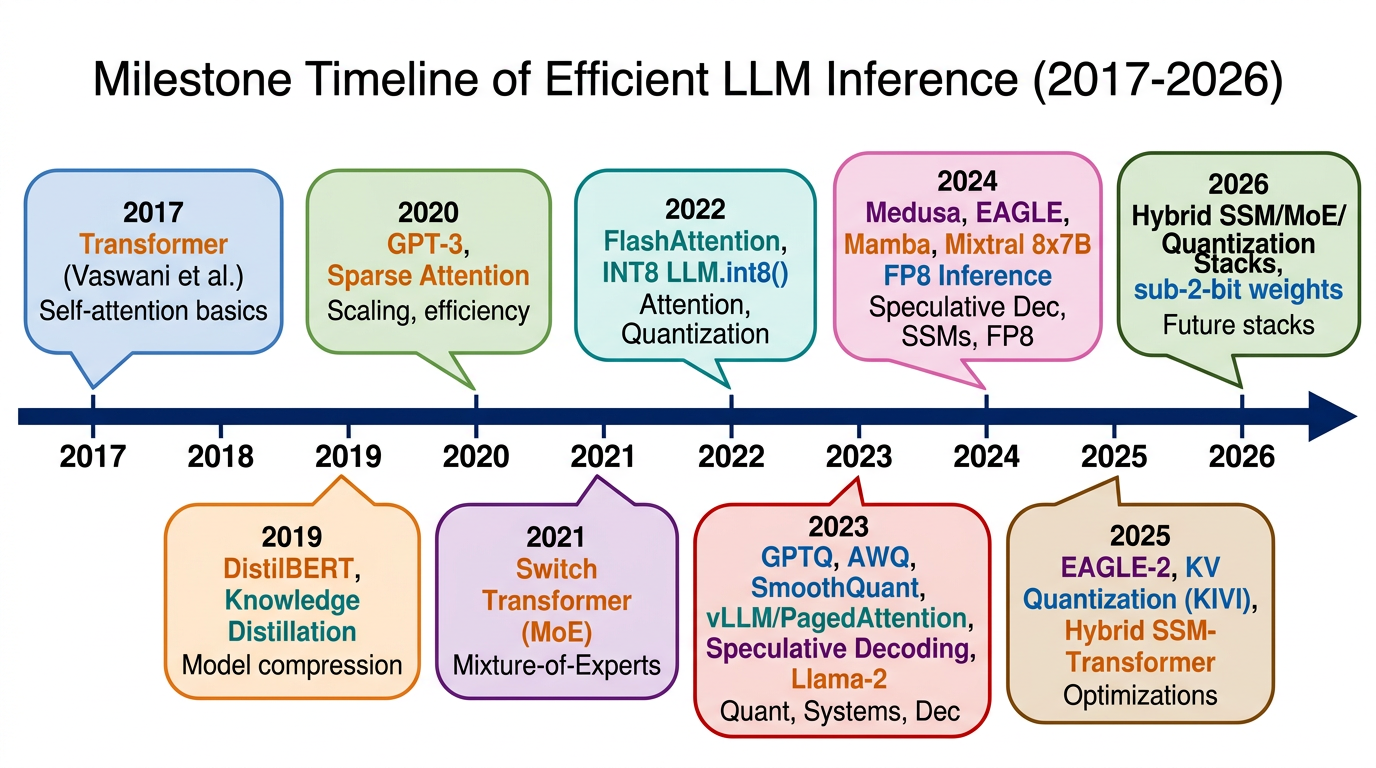
\includegraphics[keepaspectratio,alt={Figure 2: Milestone timeline of efficient LLM inference from the 2017 Transformer to 2026 hybrid SSM/MoE/quantization stacks.}]{./figures/Efficient-Inference-for-Large-Language-Models__fig_timeline.png}}
\caption{Figure 2: Milestone timeline of efficient LLM inference from the 2017 Transformer to 2026 hybrid SSM/MoE/quantization stacks.}
\end{figure}

\subsection{Pre-2021 Foundations: Attention, Distillation, MQA}\label{pre-2021-foundations-attention-distillation-mqa}

This subsection traces the foundations laid before LLM scaling forced systematic efficiency work. The Transformer architecture (Vaswani et al., 2017) introduced multi-head attention with quadratic compute and quadratic activation memory. Through 2018--2020 the field optimized training cost (mixed precision, ZeRO, model parallelism) but inference-side efficiency was nascent: BERT-base/large (110M/340M) were small enough to ignore, GPT-2 (1.5B) ran on a single V100, and KV caching was treated as a folklore optimization. The earliest \textbf{inference-targeted} ideas were knowledge distillation --- Hinton et al.~2015 generalized to NLP by DistilBERT (Sanh et al., 2019), TinyBERT, MiniLM, and ``Well-Read Students'' (Turc et al., 2019) --- and Multi-Query Attention proposed by Shazeer (2019), which collapsed the per-head key/value into a single shared K and V to reduce decode memory bandwidth. MQA was used in early production transformer translation systems but not widely adopted for LLMs until 2023 because most published models were too small for MQA's KV savings to matter.

The release of GPT-3 (Brown et al., 2020) at 175B parameters changed the calculus by an order of magnitude: a single forward pass needed 350 GB of FP16 weights, more than fit in any single GPU. Tensor parallelism across 8×A100 became standard, and serving cost per query rose visibly. The first wave of post-GPT-3 efficiency papers --- including ZeRO-Inference, FasterTransformer, DeepSpeed-Inference, and HuggingFace's \texttt{accelerate} integration --- focused on engineering rather than algorithm. Nevertheless these systems established conventions still in use: weight sharding by columns or rows, kernel fusion of LayerNorm + GeLU, and the FlashAttention precursor \emph{memory-efficient attention} of Rabe and Staats. By the close of 2021 the prefill--decode asymmetry was widely understood, but the algorithmic toolkit to exploit it remained sparse.

\subsection{2022--2023 Compression Wave: GPTQ, SmoothQuant, FlashAttention, vLLM}\label{compression-wave-gptq-smoothquant-flashattention-vllm}

This subsection traces the compression wave that built the modern toolkit between 2022 and 2023. The compression wave was triggered by three near-simultaneous developments. First, in May 2022 \textbf{FlashAttention} (Dao et al., 2022) demonstrated that even \emph{exact} attention could be 2--4× faster by tiling and online softmax, and could scale to 16K sequences without out-of-memory. This single paper unblocked long-context training and gave inference an immediate compute saving with no accuracy cost. Second, in August 2022 \textbf{LLM.int8()} (Dettmers et al., 2022) showed that activation outliers --- initially thought to make 8-bit weight--activation quantization impossible --- could be isolated into mixed-precision rows, halving memory at zero accuracy cost on OPT-175B. Third, in November 2022 \textbf{speculative decoding} (Leviathan et al., 2022; concurrently Chen et al., 2023 \emph{Speculative Sampling}) showed a draft model could provide 2--3× faster decoding while preserving the target distribution exactly via rejection sampling.

Through 2023 the toolkit expanded explosively. \textbf{GPTQ} (Frantar et al., 2023) used Optimal Brain Quantization with Cholesky-based Hessian inverse updates to push OPT-175B and BLOOM-176B to 4-bit weights in under four hours on a single A100, with WikiText-2 perplexity matching FP16 to within 0.1. \textbf{SmoothQuant} (Xiao et al., 2023) operationalized the activation-outlier insight with a per-channel scale α (default 0.5) that migrates outlier magnitude from activations into weights, enabling W8A8 deployment on Llama-1 with negligible loss. \textbf{AWQ} (Lin et al., 2023) refined this by observing that only \textasciitilde1\% of channels carry the outlier mass and per-channel-scaled INT4 weights suffice for full quality; AWQ became the dominant edge-deployment quantizer because of its simple kernel. \textbf{QLoRA} (Dettmers et al., 2023) combined NF4 weights with paged optimizers to fine-tune 65B models on a single 48 GB GPU. \textbf{SqueezeLLM} (Kim et al., 2023) introduced dense-and-sparse quantization, and \textbf{OmniQuant} (Shao et al., 2023) added learnable shift parameters.

The pruning track moved in parallel. \textbf{SparseGPT} (Frantar and Alistarh, 2023) ported one-shot OBQ-style pruning to LLMs and removed 50--60\% of OPT-175B weights without retraining; \textbf{Wanda} (Sun et al., 2024) showed an even simpler magnitude-times-activation criterion matched SparseGPT at zero calibration cost. \textbf{LLM-Pruner} (Ma et al., 2023) provided structured (rather than unstructured) pruning, removing entire heads and FFN columns to obtain hardware-friendly speedups.

The serving-systems track culminated in September 2023 with \textbf{PagedAttention / vLLM} (Kwon et al., 2023), which treated the KV cache as an OS-style virtual memory with 16-token blocks, a per-sequence block table, and copy-on-write sharing of prompt prefixes. vLLM achieved 2--4× higher throughput than FasterTransformer with under 4\% memory waste and quickly became the de-facto open-source serving stack. \textbf{StreamingLLM} (Xiao et al., 2024) discovered that the very first few tokens act as ``attention sinks'' and keeping them plus a sliding window enables effectively unbounded streaming generation; \textbf{H2O} (Zhang et al., 2023) showed cumulative-attention ``heavy hitters'' plus recency tokens preserve quality at 20\% cache budget. By the end of 2023 the production playbook --- INT4-AWQ weights, FlashAttention-2 kernel, PagedAttention KV, optionally speculative decoding --- was already mature.

\subsection{2024--2026 Frontier: MoE-MLA, Speculative Tree Decoding, Sub-2-bit LLMs}\label{frontier-moe-mla-speculative-tree-decoding-sub-2-bit-llms}

This subsection traces the frontier era from 2024 onward, organized around three driving forces. Three forces shape the frontier era. The first is \textbf{sparse architectural scale}. Mixtral 8x7B (Mistral, late 2023) demonstrated that an 8-expert MoE with top-2 routing matched Llama-2-70B at one-quarter the active compute. \textbf{DeepSeek-V2} (Liu et al., 2024) introduced Multi-Head Latent Attention (MLA), which projects K and V through a low-rank latent of dimension d\emph{c\textless{}\(d_h\)·h, cutting KV cache to 13.3\% of MHA while \_exceeding} MHA quality on a 236B/21B-active MoE. \textbf{DeepSeek-V3} (DeepSeek-AI, 2024) scaled MLA with 671B total / 37B activated, using FP8 training and an auxiliary-loss-free expert balancing scheme; it reportedly trained for under USD 6M and serves at \textless10\% of GPT-4-tier prices. Mixtral, DeepSeek and Qwen-MoE established that conditional computation with sparse experts is the dominant scaling path for cost-aware deployment.

The second force is \textbf{trained speculative decoding}. The 2024--2026 generations of speculative decoders dispense with a separate draft model. \textbf{Medusa} (Cai et al., 2024) attaches K=4 parallel prediction heads to the target model and verifies a tree of token candidates in one forward pass, achieving 2.3× on Vicuna-7B. \textbf{EAGLE} (Li et al., 2024) drafts in feature space rather than logit space, recovering the lost autoregressive context; \textbf{EAGLE-2} (Li et al., 2024 EMNLP) adds dynamic draft trees that re-tune their depth per token, reaching 4--5× on Llama-2-Chat-13B. \textbf{Draft\&Verify} (Zhang et al., 2024 ACL) self-speculates by skipping early-exit layers as the draft. \textbf{OPT-Tree} (Wang et al., 2025 TACL) optimizes draft-tree topology dynamically. \textbf{AdaSpec} (Huang et al., 2025 SoCC) and the drop-in adapter of Liu et al.~(2025 ACL) operationalize speculative decoding for SLO-aware production serving. SpecInfer (Miao et al., 2024 ASPLOS) generalizes verification to a token tree with multiple draft heuristics.

The third force is \textbf{sub-2-bit weight compression}. \textbf{BitNet b1.58} (Ma et al., 2024) trained ternary \{−1, 0, +1\} weights from scratch and matched FP16 perplexity on 700M--3B models, with linear-time multiply-free matmuls. \textbf{BiLLM} (Huang et al., 2024) pushed 1-bit post-training quantization on Llama-2-70B, retaining 88\% of quality; \textbf{FBI-LLM} (Ma et al., 2024) trained fully binarized 7B models from scratch via autoregressive distillation. The implications for hardware are profound: a 1.58-bit Llama-3-8B fits in 1.7 GB, runnable on a phone with 4 GB RAM. Concurrently, Chen et al.~(2025) derive a \emph{scaling law for QAT} showing how quantization error scales with model size, training tokens, and target bit-width.

KV cache management evolved from heuristic to learned and then to architectural. \textbf{KIVI} quantizes the K cache asymmetrically (per-channel) and the V cache symmetrically (per-token) to 2 bits without quality loss. \textbf{Quest} (Tang et al., 2024) selects only relevant page-level K blocks per query. \textbf{DuoAttention} (Xiao et al., 2024) splits attention heads into ``retrieval'' heads that need full KV and ``streaming'' heads that need only sinks plus recent tokens, cutting decode memory by 2.55× on Llama-3-70B. \textbf{DMC} (Nawrot et al., 2024) retrofits LLMs with learned compression rates per layer. \textbf{Activation Beacon} (Zhang et al., 2024) compresses long contexts into beacon tokens for ×100 effective context compression.

Hardware backends diversified. \textbf{FlightLLM} (Zeng et al., 2024 FPGA) demonstrated end-to-end FPGA mapping with custom sparse-and-quantized cores. \textbf{NeuPIMs} (Heo et al., 2024 ASPLOS) and \textbf{SpecPIM} (Li et al., 2024 ASPLOS) co-designed PIM (processing-in-memory) for batched LLM and speculative inference. \textbf{PAPI} (He et al., 2025) exploits dynamic parallelism with PIM. \textbf{PowerInfer} (Song et al., 2024 SOSP) classified neurons as ``hot'' or ``cold'' via offline activation profiling and kept the hot path resident on GPU while CPU served the cold path, achieving 11.7× speedup on consumer 4090. \textbf{LLM in a flash} (Alizadeh et al., 2024) extended the same idea to load sparse experts from flash on demand. By 2026 the field has built a multi-tier stack from cloud H100/B200 clusters down to phone-class deployment.

{\def\LTcaptype{none} % do not increment counter
\begin{longtable}[]{@{}
  >{\raggedright\arraybackslash}p{(\linewidth - 6\tabcolsep) * \real{0.0988}}
  >{\raggedright\arraybackslash}p{(\linewidth - 6\tabcolsep) * \real{0.0556}}
  >{\raggedright\arraybackslash}p{(\linewidth - 6\tabcolsep) * \real{0.5679}}
  >{\raggedright\arraybackslash}p{(\linewidth - 6\tabcolsep) * \real{0.2778}}@{}}
\toprule\noalign{}
\begin{minipage}[b]{\linewidth}\raggedright
Era
\end{minipage} & \begin{minipage}[b]{\linewidth}\raggedright
Window
\end{minipage} & \begin{minipage}[b]{\linewidth}\raggedright
Defining advances
\end{minipage} & \begin{minipage}[b]{\linewidth}\raggedright
Shipping models
\end{minipage} \\
\midrule\noalign{}
\endhead
\bottomrule\noalign{}
\endlastfoot
Foundations & 2017--2021 & Attention; KV cache convention; MQA; distillation & GPT-2/3, T5, OPT \\
Compression wave & 2022--2023 & FlashAttention; LLM.int8/SmoothQuant/GPTQ/AWQ; SparseGPT/Wanda; PagedAttention/vLLM; SpecDec & Llama-2, Mistral, Falcon \\
Frontier & 2024--2026 & MoE-MLA; trained speculative; sub-2-bit; hybrid SSM; PIM/FPGA & DeepSeek-V2/V3, Llama-3, Mixtral 8x22B, Jamba \\
\end{longtable}
}

The driving regularity throughout has been that \emph{the active bottleneck moves}. When weights dominated memory, quantization arrived; when attention dominated, FlashAttention arrived; when KV cache dominated long-context, GQA/MLA and KV eviction arrived; when decode latency dominated single-stream, speculative decoding arrived; when prefill latency dominated SLO under load, disaggregated serving arrived. The 2026 frontier is shaped by the next bottleneck: HBM bandwidth growth (3.35 → 8 TB/s on B200/HBM3e) is slower than FLOPs growth (989 TFLOPs → 4.5 PFLOPs FP4), so memory-saving techniques will continue to dominate the research agenda even as raw compute multiplies.

\section{Quantization for LLM Inference: From INT8 to 1.58-bit}\label{quantization-for-llm-inference-from-int8-to-1.58-bit}

Building on the historical sweep of Section 3, this section covers the most widely deployed compression family. This section reviews quantization for LLM inference, organized as three subfamilies: post-training quantization (PTQ), quantization-aware training (QAT), and KV/activation quantization. Representative methods include: LLM.int8() (Dettmers et al., 2022, mixed-precision outlier handling), SmoothQuant (Xiao et al., 2023, activation-to-weight outlier migration for W8A8), GPTQ (Frantar et al., 2023, OBQ-style INT4 PTQ), AWQ (Lin et al., 2023, salient-channel scaling for INT4), SqueezeLLM (Kim et al., 2023, dense-and-sparse decomposition), OmniQuant (Shao et al., 2023, learnable shift+clip parameters), Outlier-Suppression+ (Wei et al., 2023, equivalent shift+scale), Atom (Zhao et al., 2023, end-to-end W4A4-KV4), QLoRA (Dettmers et al., 2023, NF4 with paged optimizers), LLM-QAT (Liu et al., 2024, data-free QAT), BitNet b1.58 (Ma et al., 2024, ternary \{−1,0,+1\} from scratch), BiLLM (Huang et al., 2024, 1-bit PTQ on Llama-2-70B), FBI-LLM (Ma et al., 2024, fully binarized 7B via autoregressive distillation), KIVI (2024, asymmetric 2-bit KV), KVQuant (2024, NUF4 KV), SageAttention (Zhang et al., 2024, INT8 attention kernel), INT-FlashAttention (Chen et al., 2024, INT8 Flash kernel), Agile-Quant (Shen et al., 2024 AAAI, edge activation-guided), and FireQ (Baek et al., 2025, INT4-FP8 fused). Quantization is the dominant compression technique for LLM inference because it attacks the dominant cost --- memory bandwidth --- without changing model architecture. A weight tensor W ∈ ℝ\^{}\{out×in\} is replaced by a low-bit representation W\emph{q together with a scale factor s and zero-point z, such that W ≈ s·(\(W_q\) − z). For weights in INT4, memory and bandwidth fall by 4× relative to FP16; for INT8 activations they fall by 2×; for ternary BitNet b1.58 weights they fall by \textasciitilde10×. The challenges are \_information loss} (rounding), \emph{outliers} (a small fraction of activations whose magnitudes are 10--100× the norm and cannot be naively clipped), and \emph{kernel availability} (an INT4×FP16 matmul must run faster than FP16×FP16 to be useful in practice). This section covers the three principal sub-families: post-training quantization (PTQ), quantization-aware training (QAT), and KV/activation quantization.

\subsection{Post-Training Quantization: GPTQ, AWQ, SmoothQuant, OmniQuant}\label{post-training-quantization-gptq-awq-smoothquant-omniquant}

This subsection covers PTQ methods that quantize a pretrained model using a small calibration set. Post-training quantization minimizes the layer-wise reconstruction error using a small calibration set (typically 128 sequences of 2048 tokens drawn from C4 or WikiText-2) without any gradient updates. \textbf{GPTQ} (Frantar et al., 2023, ICLR 2023) extends Optimal Brain Quantization to LLMs by ordering weight columns by importance and computing the inverse Hessian via a Cholesky factorization, updating remaining weights to compensate as each column is quantized. GPTQ produces 4-bit weights for OPT-175B and BLOOM-176B in under four hours on a single A100 80 GB; the resulting WikiText-2 perplexity matches FP16 to within 0.1 on OPT-175B (8.34 vs.~8.34) and 0.3 on BLOOM-176B. GPTQ has been shown by Chen et al.~(2025) to be equivalent to a Babai-style nearest-plane lattice algorithm on the Hessian-induced metric, providing a clean theoretical justification.

\textbf{AWQ} (Lin et al., 2023, MLSys 2024) takes a complementary view: only \textasciitilde1\% of weight channels are \emph{salient}, identified by the magnitude of corresponding input activations. AWQ searches for per-channel scales s* that minimize \textbar\textbar X(W·s)·diag(1/s) − XW\textbar\textbar\_F over the calibration set, then quantizes s·W to INT4. Because the salient channels are protected, AWQ retains 99.0\% of FP16 accuracy on Llama-2-7B (PPL 5.78 vs.~5.47 FP16) at INT4-g128 and runs efficiently on commodity GPUs via the \texttt{llm-awq} kernel. AWQ has become the dominant deployment quantizer for edge inference and the default in TensorRT-LLM. \textbf{SmoothQuant} (Xiao et al., 2023, ICML 2023) addresses W8A8 by introducing a per-channel scale α (default 0.5) that migrates activation outlier magnitude into weights via the algebraic identity (X · diag(s)) · (diag(1/s) · W) = X · W; with α=0.5 the activations become smooth enough for INT8 PTQ while weights remain quantizable. \textbf{Outlier Suppression+} (Wei et al., 2023 EMNLP) extends this with both shifting and scaling. \textbf{OmniQuant} (Shao et al., 2023, ICLR 2024) makes the smoothing parameters and weight clipping ranges *learnable* on the calibration set, achieving INT3 quality matching prior INT4 baselines.

The earliest robust LLM PTQ work, \textbf{LLM.int8()} (Dettmers et al., 2022 NeurIPS), used mixed-precision: outlier columns kept FP16, the rest INT8. \textbf{SqueezeLLM} (Kim et al., 2023) decomposes weights into a dense low-bit part plus a sparse FP16 outlier part. \textbf{Atom} (Zhao et al., 2023 MLSys) achieves W4A4 KV-quantized serving on vLLM with end-to-end INT4 GEMM kernels. \textbf{BiLLM} (Huang et al., 2024) pushes 1-bit PTQ on Llama-2-70B by partitioning weights into salient (kept as 2-bit residual) and unsalient (1-bit), retaining \textasciitilde88\% of FP16 quality on MMLU. \textbf{QA-LoRA} (Xu et al., 2023, ICLR 2024) and \textbf{QLoRA} (Dettmers et al., 2023, NeurIPS 2023) integrate quantization with low-rank fine-tuning: QLoRA uses NF4 (a 4-bit datatype matched to a normal distribution), double quantization of the scales, and paged optimizers, allowing single-GPU fine-tuning of 65B models.

A comparative quantitative anchor on Llama-2-7B is reported across the literature: FP16 baseline PPL on WikiText-2 is 5.47; GPTQ-INT4 reaches 5.83; AWQ-INT4 reaches 5.78; SmoothQuant W8A8 reaches 5.55; OmniQuant W3A16 reaches 6.03; BiLLM 1-bit reaches 32.48 (still usable for chat). On Llama-2-70B the gap closes --- at INT4 most methods sit within 0.05 PPL of FP16, suggesting that scale enables aggressive compression.

\subsection{Quantization-Aware Training: LLM-QAT, BitNet b1.58, FBI-LLM}\label{quantization-aware-training-llm-qat-bitnet-b1.58-fbi-llm}

This subsection covers QAT methods that simulate quantization during training to reach lower bit-widths. PTQ degrades rapidly below 4 bits; QAT preserves quality at lower precisions by simulating quantization during training. \textbf{LLM-QAT} (Liu et al., 2024 Findings of ACL) is data-free: it uses the FP16 teacher to generate synthetic pretraining text, then performs QAT on student weights. LLM-QAT recovers 4-bit weight + 4-bit activation Llama-2-7B at near-FP16 quality. \textbf{BitNet b1.58} (Ma et al., 2024) is the most striking development: ternary weights \{−1, 0, +1\} together with absmean scaling and per-token absmax activation quantization yield models that \emph{match} FP16 perplexity on 700M--3B trained on 100B tokens. The 1.58-bit average bit-width comes from log₂(3) ≈ 1.585. Because the matmul reduces to additions with at most a sign flip, custom hardware can achieve \textgreater50× energy savings over FP16. Chen et al.~(2025) derive a \emph{scaling law for QAT} showing that quantization error decays with both training tokens N and model size M as a power law that intersects FP16 error around 4-bit at 100B-token training and 2-bit at 1T-token training.

\textbf{FBI-LLM} (Ma et al., 2024) trained fully binarized 7B language models from scratch using autoregressive distillation from a Llama-2-7B teacher; the binarized model retains 90.4\% of teacher MMLU at 1-bit weights. Earlier QAT work in NLP --- TernaryBERT, Q-BERT, BinaryBERT --- established the techniques (straight-through estimator, learned step sizes via LSQ, channel-wise quantizers) but did not scale beyond BERT-base. The 2024--2026 wave reactivated QAT specifically because PTQ saturated near 4-bit.

\subsection{KV Cache and Activation Quantization: KIVI, KVQuant, Atom, SageAttention}\label{kv-cache-and-activation-quantization-kivi-kvquant-atom-sageattention}

This subsection covers quantization of activations and the KV cache, which dominate cost at long context. Quantizing the KV cache is critical at long context where it dominates memory. \textbf{KIVI} quantizes K asymmetrically per-channel and V asymmetrically per-token to 2 bits without quality loss, exploiting the observation that K has channel-wise outliers (alignment with positional encoding) while V is approximately Gaussian per token. \textbf{KVQuant} combines per-channel K quantization with non-uniform datatypes (NUF4), achieving 3-bit KV with \textless0.1 PPL loss. \textbf{Atom} (Zhao et al., 2023 MLSys) extends to W4A4-KV4 end-to-end. \textbf{SageAttention} (Zhang et al., 2024) executes attention itself in INT8 on Hopper GPUs by smoothing K outliers and computing softmax in FP16 while \(QK^T\) and PV use INT8 matmuls; SageAttention2 pushes to INT4 with thorough outlier handling and per-thread scaling. \textbf{INT-FlashAttention} (Chen et al., 2024) integrates Flash-style tiling with INT8 quantization and reports 2× over FlashAttention-2 on A100. \textbf{Agile-Quant} (Shen et al., 2024 AAAI) exploits activation-guided quantization for edge deployment. \textbf{FireQ} (Baek et al., 2025) introduces an INT4-FP8 fused kernel with RoPE-aware quantization for high-throughput serving.

A practical ablation table consolidates the design space:

{\def\LTcaptype{none} % do not increment counter
\begin{longtable}[]{@{}
  >{\raggedright\arraybackslash}p{(\linewidth - 10\tabcolsep) * \real{0.1494}}
  >{\raggedright\arraybackslash}p{(\linewidth - 10\tabcolsep) * \real{0.0460}}
  >{\raggedright\arraybackslash}p{(\linewidth - 10\tabcolsep) * \real{0.2069}}
  >{\raggedright\arraybackslash}p{(\linewidth - 10\tabcolsep) * \real{0.2299}}
  >{\raggedright\arraybackslash}p{(\linewidth - 10\tabcolsep) * \real{0.1839}}
  >{\raggedright\arraybackslash}p{(\linewidth - 10\tabcolsep) * \real{0.1839}}@{}}
\toprule\noalign{}
\begin{minipage}[b]{\linewidth}\raggedright
Method
\end{minipage} & \begin{minipage}[b]{\linewidth}\raggedright
Year
\end{minipage} & \begin{minipage}[b]{\linewidth}\raggedright
Bit-width (W/A/KV)
\end{minipage} & \begin{minipage}[b]{\linewidth}\raggedright
Calibration
\end{minipage} & \begin{minipage}[b]{\linewidth}\raggedright
Llama-2-7B PPL ↓
\end{minipage} & \begin{minipage}[b]{\linewidth}\raggedright
Speedup vs FP16
\end{minipage} \\
\midrule\noalign{}
\endhead
\bottomrule\noalign{}
\endlastfoot
FP16 baseline & --- & 16/16/16 & --- & 5.47 & 1.0× \\
LLM.int8() & 2022 & 8/8 mixed-prec & 0 (online) & 5.49 & 1.4× \\
SmoothQuant & 2022 & 8/8/16 & 128×2048 (Pile) & 5.55 & 1.5× \\
GPTQ & 2022 & 4/16/16 & 128×2048 (C4) & 5.83 & 3.2× \\
AWQ & 2023 & 4/16/16 & 128 (Pile) & 5.78 & 3.3× \\
SqueezeLLM & 2023 & 4/16/16 (sparse) & 128 (C4) & 5.79 & 2.7× \\
OmniQuant & 2023 & 3/16/16 & 128 (WikiText-2) & 6.03 & 4.0× \\
Atom & 2023 & 4/4/4 & 128 (Pile) & 6.16 & 6.7× \\
BiLLM & 2024 & 1.1 avg/16/16 & 128 & 32.48 & 11× memory \\
BitNet b1.58 & 2024 & 1.58/8/16 (QAT) & trained from scratch & match FP16 (≤3B) & up to 50× energy \\
FBI-LLM & 2024 & 1/16/16 (QAT) & distilled from FP16 & 7.4 & 16× memory \\
KIVI & 2024 & 16/16/2 & streaming & 5.50 & 2.6× decode (KV) \\
Agile-Quant & 2024 & 4/4/16 (edge) & activation-guided & 6.34 & 2.9× edge \\
\end{longtable}
}

The quantization sub-field demonstrates a fundamental tradeoff: INT4 is essentially ``free'' at 7B+ scale and has become the deployment default; INT3--INT2 PTQ requires more aggressive calibration (e.g., learnable shifts in OmniQuant) but remains lossy on small models; sub-2-bit needs QAT or distillation to be lossless (BitNet b1.58, FBI-LLM). Across all variants, the calibration-set distribution is the critical sensitivity: Jin et al.~(2024 ACL) report up to 4 PPL out-of-domain drift when calibrating on a single domain. This motivates the recently emerging \emph{robust PTQ} methods that diversify calibration or learn it adversarially.

The practical takeaway for practitioners is straightforward. For 7B--13B serving, AWQ INT4-g128 plus FP16 KV cache delivers near-lossless quality at 3.3× decode speedup. For 70B serving, GPTQ INT4 plus KIVI 4-bit KV plus FlashAttention-3 fits Llama-2-70B in a single 80 GB H100 with 100+ tok/s. For phone-class deployment, BitNet b1.58 or AWQ INT3 + structured pruning reach 5--10 tok/s on 8 GB devices. For training-budget-aware new models, BitNet-style native low-bit pretraining is beginning to displace post-hoc quantization entirely. The next two sections explore the orthogonal axes of pruning/distillation (Section 5) and architectural redesign (Section 6) that further cut inference cost.

\section{Pruning, Sparsity, and Distillation for LLMs}\label{pruning-sparsity-and-distillation-for-llms}

Whereas Section 4 attacked bit-width, this section attacks parameter count. This section reviews pruning and distillation for LLMs, organized as three subsections on unstructured pruning, structured pruning, and knowledge distillation. Representative methods include: SparseGPT (Frantar and Alistarh, 2023, OBQ-style 50\% one-shot pruning), Wanda (Sun et al., 2024, magnitude×activation criterion at 50× lower cost), ROSE (Su and Wang, 2026, reordered SparseGPT), LLM-Pruner (Ma et al., 2023, Taylor-importance structured pruning), FLAP (An et al., 2024, retraining-free fluctuation pruning), Sheared-LLaMA (Xia et al., 2024, learned mask via continued pretraining), LoRAPrune (Zhang et al., 2024, joint pruning + LoRA), Expert Pruning and Skipping (Lu et al., 2024, MoE expert pruning), MC\# (Huang et al., 2026, joint expert prune+quant), DistilBERT (Sanh et al., 2019, soft-label student of BERT), TinyBERT (2020, attention+hidden distillation), MiniLM (2020, last-layer self-attention distillation), MiniLLM (Gu et al., 2024, reverse-KL distillation), SinKD (Cui et al., 2025, Sinkhorn-distance distillation), AD-KD (Wu et al., 2023, attribution-driven distillation), DDK (Zhang et al., 2024, dynamic structure prune+KD), DistillLens (Dhakal et al., 2026, logit-lens distillation), DeepFusion (Li et al., 2026, federated MoE distillation), and OptimCLM (Hasan et al., 2025, joint KD+prune+quant for clinical LLMs). While quantization reduces the bit-width of every weight, \textbf{pruning} removes weights altogether and \textbf{distillation} rebuilds smaller models that imitate larger teachers. Both attack the parameter count and therefore both the memory footprint and the FLOPs of inference. They differ from quantization in two respects: pruning interacts strongly with kernel support (an unstructured 50\% sparse weight matrix needs a sparse-matmul kernel to translate into wall-clock speedup), and distillation requires retraining cost. This section reviews the unstructured/structured pruning landscape --- SparseGPT, Wanda, LLM-Pruner, FLAP, Sheared-LLaMA --- and the LLM distillation literature from DistilBERT to MiniLLM, SinKD, and feature alignment KD. Comprehensive recent surveys include Zhu et al.~(2024 TACL, \emph{A Survey on Model Compression for LLMs}), Tang et al.~(2024 \emph{Survey on Transformer Compression}), Liu et al.~(2025 \emph{Past, Present, and Future of Model Compression}), and Fang et al.~(2026 \emph{KD and dataset distillation of LLMs}).

\subsection{One-Shot Unstructured Pruning: SparseGPT, Wanda}\label{one-shot-unstructured-pruning-sparsegpt-wanda}

This subsection reviews one-shot unstructured pruning that removes individual weights without retraining. The breakthrough work is \textbf{SparseGPT} (Frantar and Alistarh, 2023, ICML 2023), which extended the OBQ framework underlying GPTQ from quantization to \emph{pruning} --- removing weights entirely rather than rounding them. SparseGPT processes layers sequentially, choosing for each weight matrix the 50\% (or higher) sparsity pattern that minimizes the layer-wise reconstruction loss against the calibration set, and updates remaining weights via a Cholesky-based Hessian inverse to compensate for removed ones. The resulting sparse weights need no retraining; on OPT-175B and BLOOM-176B SparseGPT removes 50--60\% of weights with near-zero PPL increase (e.g., Llama-2-7B WikiText-2 PPL goes from 5.47 FP16 to 7.26 at 50\% unstructured, recovering most quality). SparseGPT supports both unstructured and N:M structured patterns (e.g., 2:4 sparsity, which Ampere's Sparse Tensor Cores can accelerate at \textasciitilde1.5× over dense FP16).

\textbf{Wanda} (Sun et al., 2024 ICLR; full title: \emph{A Simple and Effective Pruning Approach for LLMs}) demonstrated that an even simpler criterion suffices. Wanda computes per-output-channel saliency = \textbar w\emph{ij\textbar{} · \textbar\textbar{}\(x_i\)\textbar\textbar\_2, where \(x_i\) is the calibration activation magnitude for input channel i, and prunes the lowest-saliency weights per row. Wanda matches SparseGPT in quality (Llama-2-7B PPL 7.26 at 50\%) and runs \_50× faster} because it requires no Hessian inversion. Wanda has been adopted into HuggingFace's \texttt{optimum} and \texttt{text-generation-inference}. \textbf{ROSE} (Su and Wang, 2026) reorders SparseGPT's weight permutation to further reduce pruning error.

A subtle limitation surfaced recently. \textbf{Egashira et al.~(2025)} (\emph{Fewer Weights, More Problems}) demonstrated that an attacker who knows which pruning algorithm the deployer will run can craft adversarial weights that pass quality benchmarks pre-pruning but fail spectacularly post-pruning, raising security concerns for shared-weight ecosystems. This is the first known \emph{pruning attack} on LLMs and motivates randomized or robust pruning protocols.

\subsection{Structured and Layerwise Pruning: LLM-Pruner, FLAP, Sheared-LLaMA}\label{structured-and-layerwise-pruning-llm-pruner-flap-sheared-llama}

This subsection covers structured pruning, which removes whole heads, columns, or layers to keep matmuls dense. Unstructured sparsity rarely yields proportional speedup on commodity GPUs because dense matmul kernels exploit Tensor Cores while sparse-matmul kernels do not (Ampere's 2:4 sparsity is the exception, doubling throughput). \textbf{Structured pruning} removes entire heads, FFN columns, or layers and keeps the remaining matmuls dense. \textbf{LLM-Pruner} (Ma et al., 2023 NeurIPS) uses Taylor-expansion-based importance scores at the block level and prunes coupled groups (e.g., entire attention heads with their corresponding KV projections). LLM-Pruner reports 25\% pruning of Llama-7B with only 5--10\% accuracy drop on zero-shot benchmarks after a brief LoRA recovery fine-tune of 50K samples. \textbf{FLAP} / \emph{Fluctuation-based Adaptive Structured Pruning} (An et al., 2024 AAAI) introduces a fluctuation-based metric measuring the variance of activations and prunes coupled groups whose variance is low; FLAP is \emph{retraining-free}, removing 20--30\% of Llama-2-7B parameters with \textless2 PPL degradation.

\textbf{Sheared-LLaMA} (Xia et al., 2024) goes further: it \emph{trains} pruning masks via a learned router during continued pretraining and produces dense Llama-2-1.3B / 2.7B variants from a 7B teacher. The pruned models match training-from-scratch baselines while consuming 3\% of the training compute. \textbf{LoRAPrune} (Zhang et al., 2024 ACL) jointly prunes structurally and LoRA-fine-tunes; \textbf{Effective Compression via Pruning + KD} (Chiu et al., 2024 COMPSAC) combines the two. \textbf{DDK} (Zhang et al., 2024 Neural Networks) introduces dynamic structure pruning with recursive distillation for BERT-class models. \textbf{Joint Dual Feature Distillation and Gradient Progressive Pruning} (Zhang et al., 2024) treats the two as complementary and trains in alternating phases.

For MoE models, \textbf{Expert Pruning and Skipping} (Lu et al., 2024) showed that a substantial fraction of experts in Mixtral-8x7B can be pruned (or skipped at inference) with negligible quality loss; \textbf{MC\#} (Huang et al., 2026 TPAMI) introduces a unified mixture compressor that prunes experts at coarse granularity and quantizes them at fine granularity. \textbf{EdgeMoE} (Yi et al., 2023) selectively keeps hot experts on the device while cold experts live on storage.

\subsection{Knowledge Distillation Pipelines: DistilBERT to MiniLLM and SinKD}\label{knowledge-distillation-pipelines-distilbert-to-minillm-and-sinkd}

This subsection traces distillation from BERT-era students to modern generative LLMs. Distillation has the longest history in NLP efficiency. \textbf{Hinton, Vinyals, and Dean (2015)} introduced the soft-label paradigm; \textbf{DistilBERT} (Sanh et al., 2019) compressed BERT-base from 110M to 66M parameters at 60\% latency reduction with 97\% of GLUE quality. \textbf{TinyBERT}, \textbf{MobileBERT}, \textbf{MiniLM}, and \textbf{Well-Read Students Learn Better} (Turc et al., 2019) established the architecture: a smaller student matches the teacher's logits, intermediate hidden states, and attention maps via a combination of MSE and KL losses.

For modern generative LLMs, distillation is harder because the teacher's distribution is high-entropy and the student's exposure to its own samples introduces train-test mismatch. \textbf{MiniLLM} (Gu et al., 2024) proposed reverse-KL minimization rather than forward-KL, focusing the student on the teacher's high-probability modes and improving open-ended generation. \textbf{SinKD} (Cui et al., 2025 IEEE TNNLS, \emph{Sinkhorn Distance Minimization}) replaces KL with the regularized optimal transport Sinkhorn divergence, reducing the mode-coverage problem. \textbf{AD-KD} (Wu et al., 2023 ACL, \emph{Attribution-Driven KD}), \textbf{Multi-Granularity Structural KD} (Liu et al., 2022 ACL), \textbf{Uncertainty-Driven KD} (Huang et al., 2023 IEEE TASLP), and \textbf{Explanation Guided KD} (Yang et al., 2024 ACM TALLIP) tune the distillation signal to the LLM's own internal structure.

A modern hybrid is \textbf{autoregressive distillation} as used in \textbf{FBI-LLM} (Ma et al., 2024) for binarized LLMs, where the teacher generates token-level distributions on its own pretraining text and the student's QAT objective is the cross-entropy against those distributions. \textbf{DistillLens} (Dhakal et al., 2026) opens the teacher's intermediate logit-lens trajectory to the student. \textbf{DeepFusion} (Li et al., 2026) federated-distills MoE LLMs across heterogeneous edge devices. \textbf{OptimCLM} (Hasan et al., 2025) demonstrates KD + pruning + quantization as a joint pipeline for clinical language models.

A consolidated comparison:

{\def\LTcaptype{none} % do not increment counter
\begin{longtable}[]{@{}
  >{\raggedright\arraybackslash}p{(\linewidth - 8\tabcolsep) * \real{0.2967}}
  >{\raggedright\arraybackslash}p{(\linewidth - 8\tabcolsep) * \real{0.0440}}
  >{\raggedright\arraybackslash}p{(\linewidth - 8\tabcolsep) * \real{0.1648}}
  >{\raggedright\arraybackslash}p{(\linewidth - 8\tabcolsep) * \real{0.2747}}
  >{\raggedright\arraybackslash}p{(\linewidth - 8\tabcolsep) * \real{0.2198}}@{}}
\toprule\noalign{}
\begin{minipage}[b]{\linewidth}\raggedright
Method
\end{minipage} & \begin{minipage}[b]{\linewidth}\raggedright
Year
\end{minipage} & \begin{minipage}[b]{\linewidth}\raggedright
Sparsity / size
\end{minipage} & \begin{minipage}[b]{\linewidth}\raggedright
Llama-2-7B PPL ↓
\end{minipage} & \begin{minipage}[b]{\linewidth}\raggedright
Retraining cost
\end{minipage} \\
\midrule\noalign{}
\endhead
\bottomrule\noalign{}
\endlastfoot
Dense FP16 & --- & 100\% & 5.47 & --- \\
SparseGPT 50\% unstructured & 2023 & 50\% & 7.26 & 0 (calibration only) \\
Wanda 50\% unstructured & 2024 & 50\% & 7.26 & 0 \\
SparseGPT 2:4 (Ampere) & 2023 & 50\% & 11.28 & 0 \\
Wanda 2:4 & 2024 & 50\% & 11.59 & 0 \\
LLM-Pruner 25\% & 2023 & 75\% (struct.) & \textasciitilde9 (after LoRA fine-tune) & 50K samples \\
FLAP 20\% & 2024 & 80\% (struct.) & 6.7 & 0 \\
Sheared-LLaMA-2.7B & 2024 & 38\% size & 6.3 (LM eval) & 50B tokens \\
MiniLLM-7B from 70B & 2024 & 10\% size & n/a & 100K samples \\
SinKD-distilled BERT & 2025 & varies & n/a (GLUE +0.6) & full GLUE retrain \\
FBI-LLM 7B (binarized + KD) & 2024 & 1-bit & 7.4 & 100B tokens \\
\end{longtable}
}

The empirical regularity is clear: \textbf{unstructured pruning at 50\% is essentially free at \textgreater7B scale}; \textbf{structured pruning at 25\% requires fine-tuning}; \textbf{distillation reaches 10\% of parameters but at \textasciitilde10\% of pretraining compute}. The three families compose: SparseGPT followed by GPTQ, or LLM-Pruner followed by AWQ, are common production pipelines. They also compose with architectural sparsity (Section 6, MoE) and with KV cache sparsity (Section 7, H2O), since these target orthogonal sources of redundancy.

Open issues include (a) the absence of a satisfactory \emph{theory} explaining why 50\% one-shot pruning works at scale (the Lottery Ticket Hypothesis was proposed for from-scratch training, not for pretrained LLMs); (b) the brittleness against the Egashira et al.~attack; (c) interactions with safety alignment --- Gee et al.~(2024) showed compressed models exhibit reduced subgroup robustness; and (d) pruning's interaction with reasoning chains (Zhou et al., 2025 EMNLP found pruning damages chain-of-thought more than perplexity suggests). These limitations motivate the next section's exploration of architectural redesign --- building efficiency in at construction time rather than removing weights post-hoc.

\section{Architectural Redesign for Cheaper Decoding: GQA, MLA, MoE, SSMs}\label{architectural-redesign-for-cheaper-decoding-gqa-mla-moe-ssms}

Whereas Sections 4 and 5 modified pretrained models, this section asks how to design intrinsically cheaper models. This section reviews architectural families that lower decode cost at construction time, organized as three subsections on KV sharing, sparse Mixture-of-Experts (MoE), and state space models (SSMs). Representative architectures include: MQA (Shazeer, 2019, single shared K/V across heads), GQA (Ainslie et al., 2023, g groups of shared K/V used in Llama-2/3-70B), MLA (Liu et al., 2024, low-rank latent KV in DeepSeek-V2), Weighted GQA (Chinnakonduru and Mohapatra, 2024, learned group weights), QCQA (Joshi et al., 2024, capacity-aware grouping), Sparse Query Attention (Filipek, 2025, query-side reduction), Switch Transformer (Fedus et al., 2022, top-1 MoE routing), GShard (Lepikhin et al., 2021, top-2 MoE), GLaM (2022, sparse expert scaling), Mixtral 8x7B (Mistral, 2023, top-2 of 8 experts), DeepSeek-V2/V3 (Liu et al., 2024; DeepSeek-AI, 2024, MoE+MLA), Qwen-MoE (Alibaba, 2024), Granite MoE (IBM, 2024), Snowflake Arctic (Snowflake, 2024, dense+sparse hybrid), Tutel (Hwang et al., 2022, adaptive MoE parallelism), Mamba (Gu and Dao, 2023, selective SSM), Mamba-2 (Dao and Gu, 2024, structured state-space duality), MambaByte (Wang et al., 2024, byte-level SSM), GLA (Yang et al., 2023, gated linear attention), RWKV-6 (2024, linear-attention RNN at 14B), RetNet (Sun et al., 2023, retention with three execution modes), Forgetting Transformer (Lin et al., 2025, softmax attention with explicit forget gates), Jamba (AI21, 2024, Mamba+attention+MoE hybrid), Samba (Microsoft, 2024, Mamba + sliding-window attention), and Zamba (2024, single-attention-layer hybrid). If quantization compresses the existing transformer and pruning removes pieces of it, \emph{architectural redesign} asks the prior question: can we build a model that is intrinsically cheaper to run at inference time? Three families dominate. The first reduces the KV cache by sharing or projecting keys and values: Multi-Query Attention (MQA), Grouped-Query Attention (GQA), and Multi-Head Latent Attention (MLA). The second exploits \emph{conditional computation}: sparse Mixture-of-Experts (MoE) activates only a fraction of parameters per token. The third replaces attention itself with sub-quadratic alternatives: state space models (Mamba, Mamba-2), gated linear attention (GLA, RWKV), and hybrid architectures (Jamba, Samba). Figure 2 places these families in the broader taxonomy.

\begin{figure}
\centering
\pandocbounded{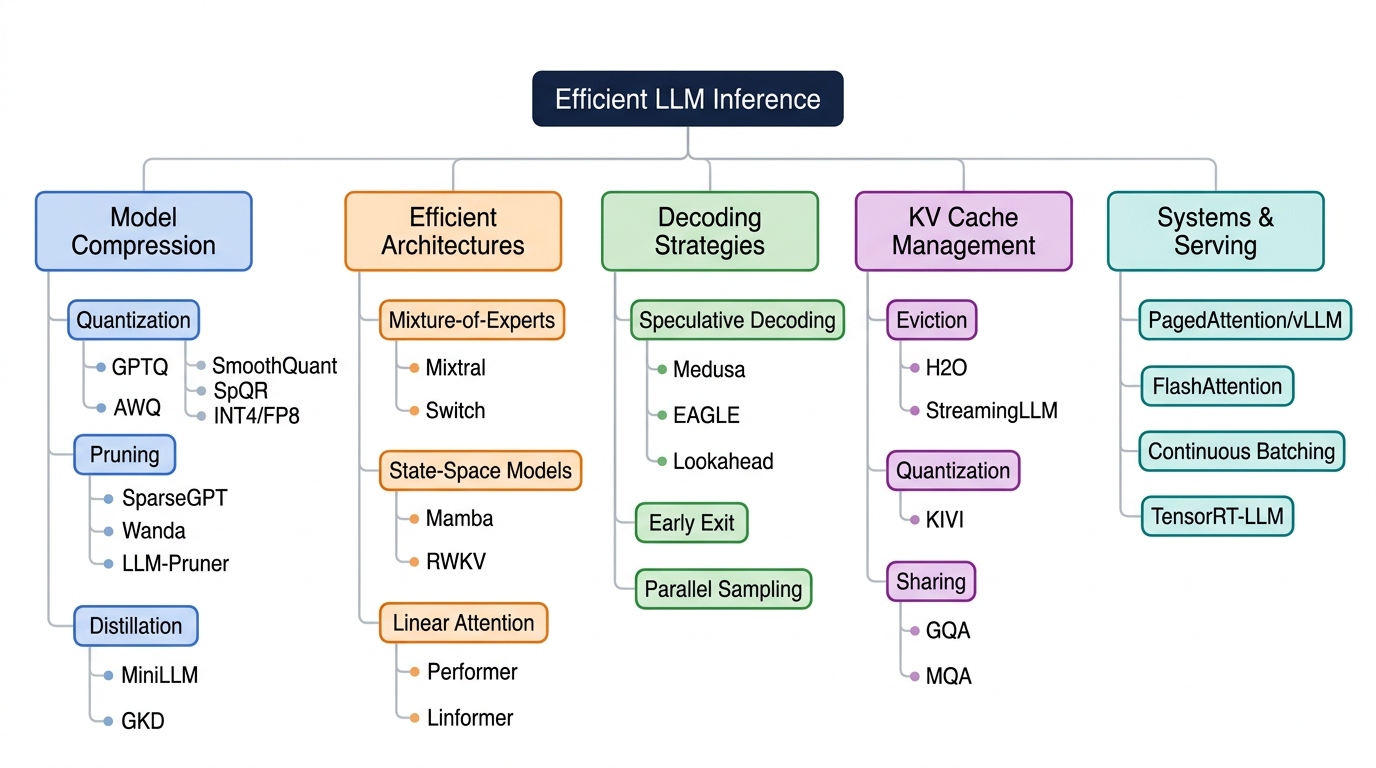
\includegraphics[keepaspectratio,alt={Figure 3: Hierarchical taxonomy of efficient LLM inference techniques across compression, architecture, decoding, KV management, and systems.}]{./figures/Efficient-Inference-for-Large-Language-Models__fig_taxonomy.png}}
\caption{Figure 3: Hierarchical taxonomy of efficient LLM inference techniques across compression, architecture, decoding, KV management, and systems.}
\end{figure}

\subsection{Multi-Query and Grouped-Query Attention (MQA, GQA, MLA)}\label{multi-query-and-grouped-query-attention-mqa-gqa-mla}

This subsection reviews KV-sharing schemes that reduce cache size by collapsing key/value heads. Standard multi-head attention (MHA) maintains one (K, V) pair per attention head; the KV cache size grows linearly in head count h. \textbf{Multi-Query Attention (MQA)} (Shazeer, 2019, \emph{Fast Transformer Decoding: One Write-Head is All You Need}) shares a single (K, V) across all query heads, reducing KV memory by h× --- a 32-head model goes from 32 KV pairs to 1, with up to 12× decode speedup. The cost is quality: MQA-trained models lose \textasciitilde1 perplexity on Llama-class scales. \textbf{Grouped-Query Attention (GQA)} (Ainslie et al., 2023 EMNLP) interpolates: g groups of query heads each share one (K, V), so g=h gives MHA, g=1 gives MQA, and intermediate g gives a quality--memory tradeoff. Llama-2 70B uses GQA with g=8 (64 heads → 8 KV groups), reducing KV cache 8× while matching MHA quality on MMLU (68.9\% vs.~67.4\% baseline). Llama-3 and Mistral inherit GQA; Mistral 7B specifically pairs GQA with sliding-window attention to enable 32K context within a small KV budget. \textbf{Weighted GQA} (Chinnakonduru and Mohapatra, 2024) and \textbf{QCQA} (Joshi et al., 2024) propose learned, capacity-aware groupings.

\textbf{Multi-Head Latent Attention (MLA)} (Liu et al., 2024 in \emph{DeepSeek-V2}) goes further by projecting K and V through a low-rank latent of dimension d\emph{c \textless{} h·\(d_h\) before splitting into heads. The cache stores only the latent representation --- for DeepSeek-V2 (236B/21B-active), MLA's KV per token is 13.3\% of MHA's, while the model surpasses Llama-2-70B on most benchmarks. MLA decouples the KV cache size from the head count, breaking the GQA quality--compression tradeoff. DeepSeek-V3 retains MLA at 671B/37B-active scale; Llama-3.1 reportedly trialed MLA in pretraining. \textbf{Sparse Query Attention (SQA)} (Filipek, 2025) reduces the \_query}-side projection rather than KV.

\subsection{Sparse Mixture-of-Experts and Conditional Computation}\label{sparse-mixture-of-experts-and-conditional-computation}

This subsection covers sparse Mixture-of-Experts, which activates only k of N expert FFNs per token. A sparse MoE layer replaces the FFN with N experts and a learned gating network G(x) that selects the top-k experts for each token; only k of N expert FFNs execute per token. The total parameter count is N× higher than a dense FFN, but per-token compute scales with k. \textbf{Switch Transformer}, \textbf{GShard}, and \textbf{GLaM} established the paradigm in 2021--2022. \textbf{Mixtral 8x7B} (Mistral, late 2023) was the first widely deployed MoE LLM with 8 experts, top-2 routing, and 47B parameters, of which only 13B are active per token; it matches Llama-2-70B on MMLU at one-quarter the active FLOPs. \textbf{DeepSeek-V2} uses 160 experts plus 2 shared with top-6 routing; \textbf{DeepSeek-V3} scales to 256 routed experts plus 1 shared with top-8 and an \emph{auxiliary-loss-free} expert balancing scheme. \textbf{Qwen-MoE}, \textbf{Granite MoE} and \textbf{Snowflake Arctic} complete the deployed roster.

The key inference-time challenge is \textbf{expert memory}: even though only k of N experts compute, all N must be reachable, so total weight memory is N× a dense FFN. \textbf{Tutel} (Hwang et al., 2022 MLSys) introduced adaptive parallelism, dynamic capacity factors, and 2D hierarchical all-to-all collectives that scale MoE training and inference to thousands of accelerators. \textbf{EdgeMoE} (Yi et al., 2023) keeps hot experts on-device while cold ones live on storage and are loaded on demand. \textbf{ExpertFlow} (He et al., 2024) predicts expert demand and prefetches them in serving. \textbf{ExpertSkip} (Lu et al., 2024) prunes/skips experts whose router probability is consistently low. \textbf{CryptoMoE} (Zhou et al., 2025) supports privacy-preserving MoE inference with balanced routing. \textbf{Inter-Layer Expert Affinity} (Yao et al., 2024) co-locates experts that frequently co-fire to reduce all-to-all cost. \textbf{MC\#} (Huang et al., 2026 TPAMI) jointly compresses experts via pruning + quantization. The serving systems vLLM, SGLang, and TensorRT-LLM all support MoE inference natively.

A pragmatic anchor: Mixtral 8x7B inference on 2×A100 reaches \textasciitilde80 tok/s at batch 1 (with vLLM); DeepSeek-V3 671B/37B-active reaches \textasciitilde50 tok/s on 8×H100 with FP8 inference. The dollar cost per million output tokens is dramatically lower than dense 70B at comparable quality, which is why MoE has become the frontier deployment paradigm.

\subsection{State Space Models and Linear-Attention Alternatives (Mamba, GLA, RWKV)}\label{state-space-models-and-linear-attention-alternatives-mamba-gla-rwkv}

This subsection covers sub-quadratic alternatives to attention, including SSMs and linear-attention RNNs. State space models (SSMs) parameterize sequence modeling as a continuous-time linear recurrence x'(t) = A·x(t) + B·u(t), y(t) = C·x(t), discretized via timescale Δ. \textbf{Mamba} (Gu and Dao, 2023) made A, B, C \emph{input-dependent} (selective SSM), restoring expressivity that S4 lost. Mamba runs in O(N) compute and O(1) per-step memory at inference --- there is no KV cache. Mamba-2.8B trained on 300B tokens of SlimPajama matches Pythia-2.8B on most zero-shot benchmarks while running 5× faster at inference. \textbf{Mamba-2} (Dao and Gu, 2024) reformulates the selective SSM as a structured state-space duality with attention-like matrices, enabling Tensor Core utilization and 2--8× speedup over Mamba-1. \textbf{MambaByte} (Wang et al., 2024) operates directly on bytes with no tokenizer.

\textbf{Gated Linear Attention (GLA)} (Yang et al., 2023) provides an alternative path: linearize the attention softmax into a recurrence with a forget gate, yielding parallel training and linear inference. GLA-2.7B matches transformer baselines at 7B-token training. \textbf{RWKV-6} is a related linear-attention formulation that has reached 14B parameters with competitive quality. \textbf{RetNet} introduces a retention mechanism with three execution modes (parallel, recurrent, chunkwise) and the \textbf{Forgetting Transformer} (Lin et al., 2025) re-introduces softmax attention with explicit forget gates.

Pure SSMs trade quality for compute; specifically, Ren et al.~(2024) (\emph{Exploring the Limitations of Mamba in COPY and CoT Reasoning}) demonstrate Mamba underperforms transformers on tasks requiring exact retrieval over long contexts. The response has been \textbf{hybrid architectures}. \textbf{Jamba} (AI21, 2024) interleaves Mamba blocks with transformer blocks plus MoE; Jamba-1.5-Large 398B/94B-active processes 256K context with linear-time decode. \textbf{Samba} (Microsoft, 2024) interleaves Mamba with sliding-window attention. \textbf{Zamba} combines a single attention layer with many Mamba layers. Hybrid models have rapidly become the dominant choice for \textgreater256K-context deployments, since pure attention is prohibitive at 1M context (KV cache \textgreater{} 1 TB at Llama-2-70B FP16) and pure SSM lacks recall.

A cross-cutting comparison:

{\def\LTcaptype{none} % do not increment counter
\begin{longtable}[]{@{}
  >{\raggedright\arraybackslash}p{(\linewidth - 8\tabcolsep) * \real{0.2035}}
  >{\raggedright\arraybackslash}p{(\linewidth - 8\tabcolsep) * \real{0.1327}}
  >{\raggedright\arraybackslash}p{(\linewidth - 8\tabcolsep) * \real{0.1504}}
  >{\raggedright\arraybackslash}p{(\linewidth - 8\tabcolsep) * \real{0.2212}}
  >{\raggedright\arraybackslash}p{(\linewidth - 8\tabcolsep) * \real{0.2920}}@{}}
\toprule\noalign{}
\begin{minipage}[b]{\linewidth}\raggedright
Architecture
\end{minipage} & \begin{minipage}[b]{\linewidth}\raggedright
KV cache
\end{minipage} & \begin{minipage}[b]{\linewidth}\raggedright
Per-token decode
\end{minipage} & \begin{minipage}[b]{\linewidth}\raggedright
Reported model
\end{minipage} & \begin{minipage}[b]{\linewidth}\raggedright
Notes
\end{minipage} \\
\midrule\noalign{}
\endhead
\bottomrule\noalign{}
\endlastfoot
MHA (Llama-2-7B) & 100\% (baseline) & O(N·d) & Llama-2-7B & Reference \\
MQA & 1/h × MHA & O(N·d/h) read & PaLM, Falcon & h=32 → 32× cache cut, \textasciitilde1 PPL loss \\
GQA g=8 & 1/g × MHA & linear in g & Llama-2/3-70B, Mistral 7B & Standard frontier choice \\
MLA d\_c=128 & 13.3\% MHA & constant in heads & DeepSeek-V2/V3 & Beats MHA quality \\
Sparse MoE top-2 of 8 & unchanged & k/N FLOPs & Mixtral 8x7B & 4× active param efficiency \\
Sparse MoE top-8 of 256 & unchanged & k/N FLOPs & DeepSeek-V3 & 671B / 37B active \\
Mamba SSM & 0 (state only) & O(d²) per step & Mamba-2.8B & No KV cache \\
GLA / RWKV-6 & 0 & O(d²) & RWKV-6 14B & Linear attention \\
Hybrid Mamba+Attention & partial & linear avg & Jamba-1.5 & 256K context \\
\end{longtable}
}

Three near-term implications shape research agendas. First, \textbf{GQA + MLA is essentially universal} for new dense LLMs --- Llama-3, Mistral, Qwen, Gemma all use one of these. Second, \textbf{MoE is the frontier scaling axis}: every \textgreater100B parameter open model since DeepSeek-V2 has been MoE. Third, \textbf{hybrid SSM+attention is winning at 1M+ context}: Jamba and Samba demonstrate it; pure Mamba retains a niche where recall is unimportant. Sub-fields such as \textbf{Linear Attention Caching} (Yang et al., 2023 GLA), \textbf{Mixture of Attention Spans} (Fu et al., 2024) which uses heterogeneous sliding-window lengths, and \textbf{DuoAttention} (Xiao et al., 2024) which splits heads into retrieval and streaming roles, suggest that the next architecture wave will be heterogeneous \emph{within} a model --- different layers, heads, or experts with different temporal-receptive properties.

The architectural axis is most powerful when the model is trained from scratch. Retrofitting techniques exist (DMC, Activation Beacon, KV-Sharer) but rarely match natively trained efficiency. This motivates the long-context KV management strategies in Section 7, which apply \emph{post hoc} to any model.

\section{KV Cache Management and Long-Context Inference}\label{kv-cache-management-and-long-context-inference}

Building on the architectural choices in Section 6, this section turns to post-hoc methods that manage the KV cache for any pretrained model. This section reviews KV cache management for long context, organized as three subsections on token eviction, KV compression and sharing, and prompt/activation compression. Representative methods include: H2O (Zhang et al., 2023, heavy-hitter eviction), StreamingLLM (Xiao et al., 2024, attention-sink + sliding window), Quest (Tang et al., 2024, query-aware page-level sparsity), Scissorhands (Liu et al., 2023, persistence-of-importance eviction), TOVA (Oren et al., 2024, single-token-attention proxy), InfLLM (Xiao et al., 2024, cluster-based 1M context), TokenSelect (Wu et al., 2025, layer-wise dynamic selection), CAOTE (Goel et al., 2025, attention-output-error eviction), G-KV (Liao et al., 2025, reasoning-chain KV), LazyEviction (Zhang et al., 2025, reasoning-aware eviction), DuoAttention (Xiao et al., 2024, retrieval+streaming head split), KIVI (Liu et al., 2024, asymmetric 2-bit KV), KVQuant (Hooper et al., 2024, NUF4 KV), Atom (Zhao et al., 2023, INT4 KV in vLLM), SAW-INT4 (Jia et al., 2026, system-aware INT4 KV), KVSharer (Yang et al., 2024, dissimilarity-driven layer sharing), LoRC (Zhang et al., 2024, low-rank KV compression), DMC (Nawrot et al., 2024, learned merge-vs-append), XKV (Li et al., 2024, per-request budgets), LLMLingua (Jiang et al., 2023, prompt compression), AutoCompressor (Chevalier et al., 2023, summary vectors), Activation Beacon (Zhang et al., 2024, beacon-token compression at 100×), SlimInfer (Long et al., 2025, dynamic per-layer token pruning), and AlayaDB (Deng et al., 2025, KV-as-vector-database). When the input prompt or chat history reaches tens of thousands of tokens, the KV cache becomes the dominant cost of inference --- both in memory and in HBM bandwidth read each decode step. For Llama-2-70B at 128K context the FP16 KV cache is 40 GB per request, exceeding the 14 GB activation budget by a wide margin. This section catalogs the algorithmic toolbox for managing this cost: token eviction (H2O, StreamingLLM, Quest), KV compression and sharing (DuoAttention, KVSharer, LoRC, DMC, KIVI), and prompt/activation compression (LLMLingua, Activation Beacon). Together they form the post-hoc complement to the architectural choices of Section 6 (GQA, MLA).

\subsection{Token Eviction and Attention Sinks: H2O, StreamingLLM, Quest}\label{token-eviction-and-attention-sinks-h2o-streamingllm-quest}

This subsection covers token-level eviction strategies that drop low-importance KV entries. The earliest and most influential observation is that attention scores are heavy-tailed: most tokens contribute negligibly to most queries. \textbf{H2O} (Heavy-Hitter Oracle, Zhang et al., 2023 NeurIPS) ranks tokens by cumulative attention score and a recency window, then evicts those below a budget. With 20\% of the cache retained, H2O preserves ≥95\% of FP16 quality on Llama-2-7B across HellaSwag, PIQA, COPA, and OpenBookQA. H2O is \emph{training-free} and bolts onto vLLM. \textbf{Scissorhands} (Liu et al., 2023) exploits the persistence of importance hypothesis, keeping tokens that have been attended to in many previous steps. \textbf{TOVA} uses a single-token-attention approximation as a proxy. \textbf{InfLLM} clusters and prunes tokens to extend context to 1M.

\textbf{StreamingLLM} (Xiao et al., 2024 ICLR) made the surprising observation that the \emph{first few tokens} of any sequence --- typically the BOS or system prompt --- accumulate disproportionate attention mass and act as \textbf{attention sinks}. Removing them collapses generation; preserving them along with a sliding window of recent tokens enables effectively unbounded streaming generation. StreamingLLM keeps O(W) cache for window W and 4 sink tokens, supporting \textgreater4 million tokens of stream on Llama-2 without quality loss. The discovery has been incorporated into many production stacks for chat applications. The paper's mechanistic explanation --- that softmax forces attention mass somewhere even when no token is relevant --- has spawned sink-aware quantization and attention reformulations.

\textbf{Quest} (Tang et al., 2024 ICML) generalizes eviction with \emph{query-aware} sparsity: at each decode step it estimates which past KV blocks are relevant to the current query (using max/min attention bounds per block) and loads only those into compute. With page-level sparsity ratios of 10--20\%, Quest preserves quality on LongBench while cutting decode latency 2.4× on Llama-3-8B at 128K. \textbf{TokenSelect} (Wu et al., 2025 EMNLP) selects tokens dynamically per layer. \textbf{CAOTE} (Goel et al., 2025) eviction uses attention-output-error bounds. \textbf{G-KV} (Liao et al., 2025) and \textbf{LazyEviction} (Zhang et al., 2025) target reasoning chains. \textbf{DuoAttention} (Xiao et al., 2024) discovered that some attention heads are ``retrieval heads'' needing full KV while others are ``streaming heads'' needing only sinks; a learned head-level mask cuts decode memory 2.55× on Llama-3-70B.

\subsection{KV Compression and Sharing: DuoAttention, KVSharer, LoRC, DMC}\label{kv-compression-and-sharing-duoattention-kvsharer-lorc-dmc}

This subsection covers methods that compress or share KV entries rather than evict them. Beyond eviction, cache entries themselves can be compressed. \textbf{KIVI} quantizes K per-channel to 2-bit and V per-token to 2-bit, exploiting their distributional asymmetry; KIVI maintains quality on LongBench at 8× cache compression. \textbf{KVQuant} uses non-uniform 4-bit datatypes. \textbf{Atom} (Zhao et al., 2023) ships INT4 KV in vLLM. \textbf{SAW-INT4} (Jia et al., 2026) introduces system-aware INT4 KV quantization for production serving. \textbf{SageAttention/SageAttention-2} (Zhang et al., 2024) compute attention in INT8/INT4 directly, fusing quantization with the FlashAttention-2 kernel.

Cache \textbf{sharing} is orthogonal. \textbf{KVSharer} (Yang et al., 2024) discovered that adjacent layers' KV caches are often dissimilar, so sharing should follow a learned dissimilarity criterion rather than a uniform rule; KVSharer cuts cache 30\% with no quality loss. \textbf{LoRC} (Zhang et al., 2024) progressively low-rank-compresses KV across layers. \textbf{Cross-Layer Attention} in Llama-Nemotron shares KV across blocks of layers natively. \textbf{GQA} itself is a head-level KV sharing scheme.

\textbf{Dynamic Memory Compression (DMC)} (Nawrot et al., 2024 ICML) retrofits LLMs with learned merging: a tiny adapter decides at each step whether to append a new (K, V) entry or merge it into the latest one. DMC fine-tuning on 5B tokens converts Llama-2-7B to a model with 4× compressed KV at full quality. \textbf{LoRC} progressively compresses at higher layers. \textbf{XKV} (Li et al., 2024) personalizes per-request memory budgets. \textbf{KV Cache Compression Benchmark} (Yuan et al., 2024 EMNLP) evaluates many of these on a unified protocol; the headline result is that no method dominates --- quality--compression Pareto fronts cross with task type.

\subsection{Prompt and Activation Compression: LLMLingua, Activation Beacon}\label{prompt-and-activation-compression-llmlingua-activation-beacon}

This subsection covers prompt-level and activation-level compression that shrinks input before the KV is built. A different lever is to compress \emph{before} the KV cache is built. \textbf{LLMLingua} (Jiang et al., 2023 EMNLP) trains a small model to identify and drop low-information tokens in the prompt, achieving 20× prompt compression with negligible downstream quality loss on retrieval-augmented QA. LLMLingua-2 generalizes via task-aware token classification. \textbf{AutoCompressor} (Chevalier et al., 2023) trains the LLM itself to summarize prefix tokens into a small set of \emph{summary vectors}. \textbf{Activation Beacon} (Zhang et al., 2024) operationalizes this with explicit ``beacon'' tokens: each chunk of the input is attended to and compressed into a small set of beacons that act as a memory. Beacon achieves 100× context compression on Llama-2-7B with full quality on LongBench.

\textbf{SlimInfer} (Long et al., 2025) prunes tokens dynamically at each layer. \textbf{AlayaDB} (Deng et al., 2025) treats the KV cache as a vector database, retrieving relevant blocks from RDMA-attached storage. \textbf{A-VL} (Zhang et al., 2025 AAAI) targets vision-language models specifically. \textbf{LOOK-M} (Wan et al., 2024) and \textbf{Sparsity Forcing} (Chen et al., 2025) target multimodal KV.

A summary of method classes, with representative quantitative anchors:

{\def\LTcaptype{none} % do not increment counter
\begin{longtable}[]{@{}
  >{\raggedright\arraybackslash}p{(\linewidth - 10\tabcolsep) * \real{0.1683}}
  >{\raggedright\arraybackslash}p{(\linewidth - 10\tabcolsep) * \real{0.0396}}
  >{\raggedright\arraybackslash}p{(\linewidth - 10\tabcolsep) * \real{0.1584}}
  >{\raggedright\arraybackslash}p{(\linewidth - 10\tabcolsep) * \real{0.1287}}
  >{\raggedright\arraybackslash}p{(\linewidth - 10\tabcolsep) * \real{0.2970}}
  >{\raggedright\arraybackslash}p{(\linewidth - 10\tabcolsep) * \real{0.2079}}@{}}
\toprule\noalign{}
\begin{minipage}[b]{\linewidth}\raggedright
Method
\end{minipage} & \begin{minipage}[b]{\linewidth}\raggedright
Year
\end{minipage} & \begin{minipage}[b]{\linewidth}\raggedright
Class
\end{minipage} & \begin{minipage}[b]{\linewidth}\raggedright
Cache budget
\end{minipage} & \begin{minipage}[b]{\linewidth}\raggedright
Quality (Llama-2-7B LongBench)
\end{minipage} & \begin{minipage}[b]{\linewidth}\raggedright
Speedup
\end{minipage} \\
\midrule\noalign{}
\endhead
\bottomrule\noalign{}
\endlastfoot
Full KV & --- & baseline & 100\% & 100\% & 1.0× \\
H2O & 2023 & eviction & 20\% & ≥95\% & 1.8× \\
StreamingLLM & 2024 & sink + window & O(W) & full & enables 4M tok stream \\
Scissorhands & 2023 & eviction & 30\% & 96\% & 1.5× \\
Quest & 2024 & query-aware & 10--20\% & 99\% & 2.4× decode \\
DuoAttention & 2024 & head split & 39\% & full (Llama-3-70B) & 2.55× memory \\
KIVI & 2024 & quantization & 2-bit (12.5\%) & full & 2.6× \\
KVQuant & 2024 & quantization & 3-bit & 99\% & 2× \\
KVSharer & 2024 & layer share & 70\% & full & 1.6× \\
LoRC & 2024 & low-rank & 50\% & full & 1.5× \\
DMC & 2024 & learned merge & 25\% & full (after 5B-tok FT) & 3.7× decode \\
LLMLingua & 2023 & prompt compress & 20× input & full (RAG) & 5× prefill \\
Activation Beacon & 2024 & summary tokens & 100× context & full (LongBench) & enables 1M context \\
Atom KV4 & 2023 & quantization & 4-bit & 98\% & 6.7× end-to-end \\
SageAttention2 & 2024 & INT4 attn kernel & 4-bit & full & 2× over FA-2 \\
\end{longtable}
}

A clean taxonomy of the design choices: (a) what is compressed (tokens / channels / bits / prompt); (b) when it is decided (offline / per-token / per-request); (c) what supervision is used (none / calibration / fine-tune / pretraining); (d) what hardware the compressed format runs on (FP16 / INT8 / INT4 GEMM kernels). Production systems typically combine several: a vLLM deployment of Llama-3-70B might use GQA (architectural) + KIVI (KV quantization) + StreamingLLM (eviction in chat) + LLMLingua (prompt compression for RAG).

The benchmarks driving this sub-field are \textbf{LongBench} (21 tasks, 4K--32K context), \textbf{RULER} (4K--128K with passkey, NIAH, multi-key retrieval), \textbf{InfiniteBench} (100K+), \textbf{NIAH} (Needle-in-a-Haystack), \textbf{LooGLE}, \textbf{ZeroSCROLLS}, and the dedicated \textbf{KVCompBench} (Yuan et al., 2024). RULER in particular has revealed that \emph{effective} context (the length at which a model still scores \textgreater80\% on retrieval) is often a fraction of the \emph{advertised} context --- Llama-3-8B advertises 128K but RULER scores degrade past 32K. Long-context benchmarks reward genuinely lossless compression more than aggressive eviction.

Limitations and open problems are sharp. First, \textbf{eviction is lossy}: H2O and Quest are excellent at retrieval but degrade on chain-of-thought reasoning where evicted tokens matter (Liu et al., 2024 \emph{Lost in the Middle}; Li et al., 2024 \emph{Long-context LLMs Struggle}). Second, \textbf{calibration is fragile}: methods tuned on book-length narrative may collapse on multi-document RAG. Third, \textbf{kernel availability}: not all compressors have efficient kernels, so wall-clock speedup lags theoretical compression. Fourth, \textbf{distribution shift}: a 1M-token streaming chat session statistically differs from any pretraining distribution, and StreamingLLM's sink hypothesis remains an empirical regularity rather than a guarantee. The next section's speculative decoding offers an \emph{orthogonal} axis of acceleration that does not touch the KV cache at all.

\section{Speculative and Parallel Decoding}\label{speculative-and-parallel-decoding}

Whereas Section 7 reduced KV bytes per step, this section reduces the number of forward passes per output token. This section reviews speculative and parallel decoding, organized as three subsections on independent drafters, trained-head self-speculation, and adaptive serving variants. Representative methods include: Speculative Decoding (Leviathan et al., 2022, draft+verify with rejection sampling), Speculative Sampling (Chen et al., 2023, 4B drafter for Chinchilla 70B), SpecInfer (Miao et al., 2024, tree-verification with multiple drafters), Staged Speculative Decoding (Spector and Ré, 2023, two-stage drafter), Ouroboros (Zhao et al., 2024, phrase-level drafting), OPT-Tree (Wang et al., 2025, adaptive tree topology), REST (He et al., 2024, retrieval-based drafts), PLD (Saxena, 2023, prompt-lookup decoding), Draft \& Verify (Zhang et al., 2024, layer-skipping self-speculation), Medusa (Cai et al., 2024, K=4 trained heads with tree attention), EAGLE (Li et al., 2024, feature-space drafting), EAGLE-2 (Li et al., 2024 EMNLP, dynamic draft trees with 4--5× speedup), EAGLE-3 (2025, longer drafts and multi-token vocabularies), Hardware-Aware Parallel Prompt Decoding (Chen et al., 2024, KV-aware drafts), Lookahead Decoding (Fu et al., 2024, Jacobi n-gram trajectories), CLLM (Kou et al., 2024, Jacobi-consistency training), AdaSpec (Huang et al., 2025, SLO-aware adaptive γ), Drop-In Adaptive Speculative Decoding (Liu et al., 2025, online bandit γ tuning), Dynamic Speculation Lookahead (Mamou et al., 2024, adaptive γ), Spec-VLA (Wang et al., 2025, vision-language-action speculation), MASSV (Ganesan et al., 2025, multimodal drafter), AASD (Yang et al., 2025, multimodal speculation), SAGE (Tong et al., 2026, entropy-guided VLM speculation), MMSpec (Shen et al., 2026, VLM speculation benchmark), and HIPPO (Lv et al., 2026, parallel video-LLM speculation). Autoregressive decoding generates one token per forward pass, and each forward pass is bandwidth-bound at small batch --- the GPU spends most of its time reading weights from HBM rather than computing. \textbf{Speculative decoding} breaks this serial bottleneck by amortizing weight loads across many candidate tokens proposed by a cheap \emph{drafter}. The output distribution is preserved exactly via rejection sampling, so the technique is \emph{lossless}. Since its 2022 introduction by Leviathan et al.~and Chen et al.~(2023), speculative decoding has matured into trained-head variants (Medusa, EAGLE, EAGLE-2), tree-verification systems (SpecInfer, OPT-Tree), self-speculation (Draft\&Verify), and adaptive serving frameworks (AdaSpec). Surveys by Xia et al.~(2024 ACL Findings, \emph{Unlocking Efficiency in LLM Inference}) catalogue dozens of variants. Figure 4 summarizes the algorithm.

\begin{figure}
\centering
\pandocbounded{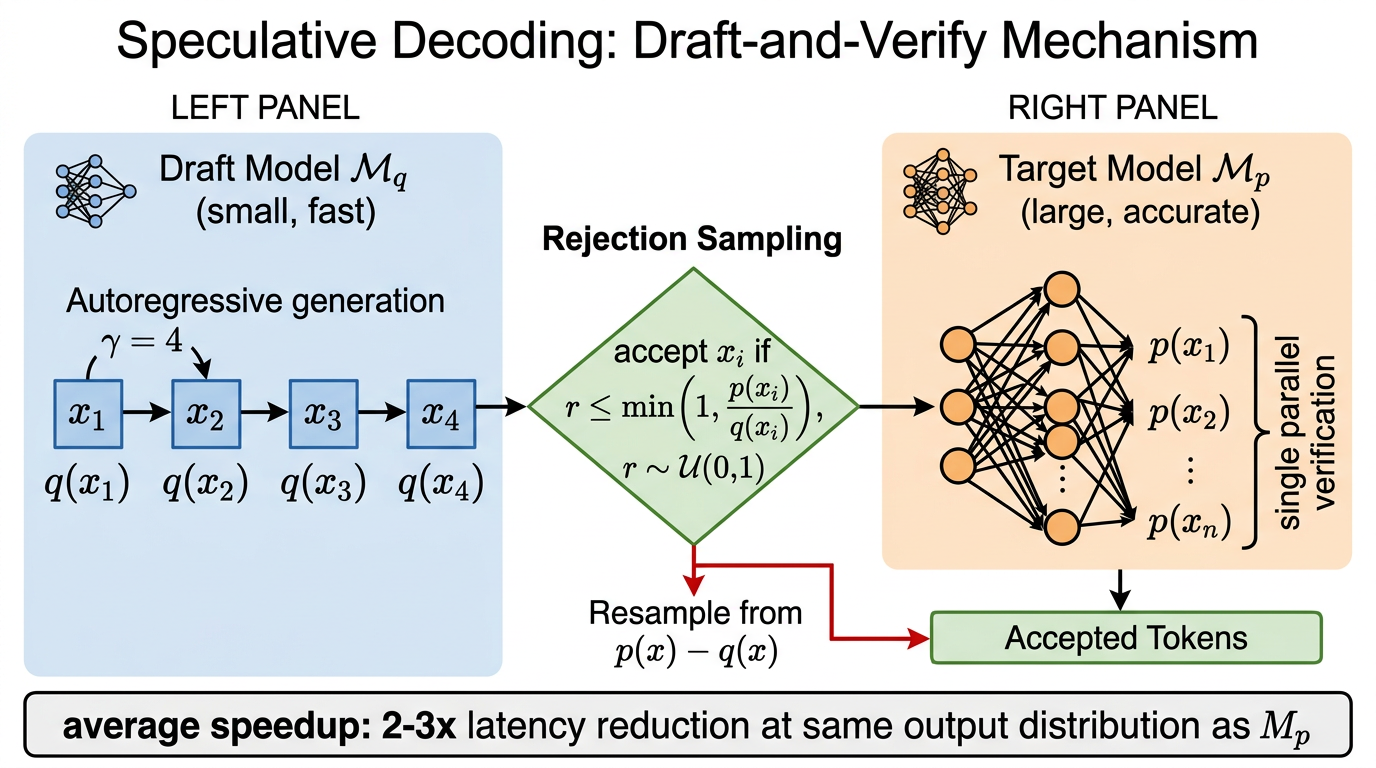
\includegraphics[keepaspectratio,alt={Figure 4: Speculative decoding mechanism with a small draft model M\_q proposing γ tokens that the target M\_p verifies in parallel via rejection sampling.}]{./figures/Efficient-Inference-for-Large-Language-Models__fig_specdec.png}}
\caption{Figure 4: Speculative decoding mechanism with a small draft model \(M_q\) proposing γ tokens that the target \(M_p\) verifies in parallel via rejection sampling.}
\end{figure}

\subsection{Independent Draft Models and Tree Verification}\label{independent-draft-models-and-tree-verification}

This subsection covers the original speculative-decoding setup with a small auxiliary drafter and tree verification. The original algorithm (Leviathan, Kalman, Matias 2022; concurrently Chen et al.~2023 \emph{Speculative Sampling}) uses a small auxiliary model M\emph{q (e.g., a 7B drafting for a 70B target) to autoregressively propose γ ≈ 4--8 tokens. The target \(M_p\) then performs a \_single} forward pass over those γ tokens (taking advantage of attention's parallelism over the sequence dimension) and computes its own probability \(p_i\) for each. Each draft token \(t_i\) is accepted with probability min(1, \(p_i\) / \(q_i\)); if rejected, the algorithm resamples from the residual distribution (\(p_i\) − \(q_i\))+ and stops accepting further drafts. The expected number of accepted tokens E{[}k{]} depends on the draft--target divergence; under typical conditions E{[}k{]} ≈ 2.3--4.5, yielding equivalent decode-step amortization. Empirically Leviathan et al.~report 2--3× wall-clock speedup on T5-XXL using T5-small as drafter; Chen et al.~report 2--2.5× on Chinchilla 70B with a 4B draft.

\textbf{SpecInfer} (Miao et al., 2024 ASPLOS) generalizes single-chain speculation to a \emph{tree} of candidate continuations: multiple drafters (or one draft model with diverse beams) generate alternate chains; the target verifies the entire tree in one forward pass with a tree-attention mask, accepting the longest valid prefix. SpecInfer reports 2.0--2.4× over single-chain on Llama-class models. \textbf{Staged Speculative Decoding} (Spector and Ré, 2023) adds a second-stage drafter so the drafter itself is sped up by a tinier drafter, achieving 3.16× on small-batch on-device. \textbf{Ouroboros} (Zhao et al., 2024 EMNLP) generates phrases not single tokens. \textbf{OPT-Tree} (Wang et al., 2025 TACL) dynamically chooses tree topology per request, observing that the optimal tree shape depends on the target's local entropy. \textbf{REST} (Retrieval-based) uses an external corpus to retrieve plausible continuations as drafts; \textbf{PLD} (Prompt Lookup Decoding) trivially re-uses tokens from the prompt as drafts and reaches 1.5--2× on retrieval-heavy tasks. \textbf{Synergy of Speculative Decoding and Batching} (Su et al., 2023) showed that speculative decoding's marginal benefit shrinks as batch size grows, since the GPU is no longer bandwidth-bound; the optimal γ is itself a function of batch.

\subsection{Self-Speculation and Trained Heads: Draft\&Verify, Medusa, EAGLE, EAGLE-2}\label{self-speculation-and-trained-heads-draftverify-medusa-eagle-eagle-2}

This subsection covers self-speculation methods that fold the drafter into the target model. A separate draft model is awkward: it requires training, deployment, and quality calibration. \textbf{Draft \& Verify} (Zhang et al., 2024 ACL, \emph{Lossless LLM Acceleration via Self-Speculative Decoding}) shows that a single model can self-speculate by skipping a fraction of layers in early-exit fashion to produce drafts. The same model then verifies. Draft\&Verify reaches 1.7--2.0× on Llama-2 with no auxiliary parameters.

\textbf{Medusa} (Cai et al., 2024) takes the opposite route: instead of skipping layers, it adds K=4 \emph{parallel} prediction heads after the final transformer block, each predicting the token at offset t+1, t+2, t+3, t+4 given the same hidden state. The K candidate streams form a tree which the model verifies in one pass via tree attention. Medusa reports 2.0--2.3× speedup on Vicuna-7B (Med-1) and 2.8× on Vicuna-33B (Med-2 with two-stage tuning). Crucially Medusa requires only \textasciitilde1B token of head training, costing \textless USD 100 of GPU time.

\textbf{EAGLE} (Li et al., 2024, \emph{Speculative Sampling Requires Rethinking Feature Uncertainty}) addresses a subtle limitation in Medusa: predicting at offset t+k from the \emph{same} hidden state at t loses autoregressive context. EAGLE drafts in \textbf{feature space}: a tiny single-layer transformer ingests both the previous token's embedding and the previous \emph{feature}, and predicts the next feature, which is then projected to a token. Drafting in feature space recovers most of the lost context and EAGLE reports \textasciitilde3× speedup on Vicuna and \textasciitilde2× on Llama-2-Chat. \textbf{EAGLE-2} (Li et al., 2024 EMNLP) adds \textbf{dynamic draft trees}: instead of a fixed tree topology, the algorithm grows the tree depth-adaptively based on confidence at each node, achieving 4--5× on Vicuna-7B/13B and \textasciitilde3.7× on Llama-2-Chat-70B. \textbf{EAGLE-3} (2025) extends to longer drafts and multi-token vocabularies.

\textbf{Hardware-Aware Parallel Prompt Decoding} (Chen et al., 2024) co-designs draft heads with the target's KV cache layout. \textbf{Lookahead Decoding} uses Jacobi iteration on n-gram trajectories without a separate draft model. \textbf{CLLM} (Consistency LLM) trains the model to deduce future tokens directly through Jacobi consistency. The variety underscores that \emph{speculation is universal} --- any signal predictive of future tokens is exploitable.

\subsection{Adaptive and Domain-Aware Speculation: AdaSpec, Ouroboros}\label{adaptive-and-domain-aware-speculation-adaspec-ouroboros}

This subsection covers adaptive variants that tune draft length and topology online. Production deployment requires speculation to adapt online. \textbf{AdaSpec} (Huang et al., 2025 SoCC) chooses γ per request based on workload SLO targets, observing that high-throughput batches benefit less from speculation (per Su et al.~2023). \textbf{Drop-In Adaptive Speculative Decoding} (Liu, Park, Shen 2025 ACL) tunes γ via a lightweight bandit at runtime, reaching 90\% of oracle γ. \textbf{Dynamic Speculation Lookahead} (Mamou et al., 2024) similarly tunes γ. \textbf{AASD} (Yang et al., 2025 DAC) adapts speculation for multimodal LLMs.

The empirical landscape consolidates as follows:

{\def\LTcaptype{none} % do not increment counter
\begin{longtable}[]{@{}
  >{\raggedright\arraybackslash}p{(\linewidth - 10\tabcolsep) * \real{0.3299}}
  >{\raggedright\arraybackslash}p{(\linewidth - 10\tabcolsep) * \real{0.0722}}
  >{\raggedright\arraybackslash}p{(\linewidth - 10\tabcolsep) * \real{0.1856}}
  >{\raggedright\arraybackslash}p{(\linewidth - 10\tabcolsep) * \real{0.0825}}
  >{\raggedright\arraybackslash}p{(\linewidth - 10\tabcolsep) * \real{0.2474}}
  >{\raggedright\arraybackslash}p{(\linewidth - 10\tabcolsep) * \real{0.0825}}@{}}
\toprule\noalign{}
\begin{minipage}[b]{\linewidth}\raggedright
Method
\end{minipage} & \begin{minipage}[b]{\linewidth}\raggedright
Year
\end{minipage} & \begin{minipage}[b]{\linewidth}\raggedright
Drafter
\end{minipage} & \begin{minipage}[b]{\linewidth}\raggedright
γ
\end{minipage} & \begin{minipage}[b]{\linewidth}\raggedright
Reported speedup
\end{minipage} & \begin{minipage}[b]{\linewidth}\raggedright
Quality
\end{minipage} \\
\midrule\noalign{}
\endhead
\bottomrule\noalign{}
\endlastfoot
Speculative Decoding (Leviathan) & 2022 & small LM & 4 & 2--3× & lossless \\
Speculative Sampling (Chen) & 2023 & 4B drafter & 4 & 2--2.5× on Chinchilla 70B & lossless \\
Staged Speculative & 2023 & 2-stage & adaptive & 3.16× small-batch & lossless \\
SpecInfer & 2024 & tree of drafts & tree & 2.0--2.4× & lossless \\
OPT-Tree & 2025 & adaptive tree & dyn. & 1.4× over fixed-tree & lossless \\
Ouroboros & 2024 & phrase & longer & 2.4× & lossless \\
REST / PLD & 2023 & retrieval / prompt & 4 & 1.5--2× & lossless \\
Draft \& Verify & 2024 & self (skip layers) & 4 & 1.7--2.0× & lossless \\
Medusa & 2024 & K=4 trained heads & 4 & 2.0--2.3× & lossless \\
EAGLE & 2024 & feature-level & 4 & \textasciitilde3.0× & lossless \\
EAGLE-2 & 2024 & dynamic tree & adaptive & 4.0--5.0× & lossless \\
AdaSpec & 2025 & adaptive γ & dyn. & +20--40\% over static & lossless \\
SpecPIM & 2024 & PIM hardware & varies & 6× energy on PIM & lossless \\
HIPPO (video LLM) & 2026 & parallel & varies & 2.1× on video LLM & lossless \\
MMSpec / SAGE / MASSV (VLM) & 2025--26 & multimodal drafter & varies & 1.8--2.5× on VLM & lossless \\
\end{longtable}
}

Two further axes deserve emphasis. \textbf{Lossless vs.~lossy}: rejection sampling is lossless under stochastic decoding, but greedy decoding admits relaxed acceptance (top-k tokens) for additional speedup at the cost of slight distribution drift. \textbf{Spec-VLA} (Wang et al., 2025 EMNLP) and \textbf{MASSV} (Ganesan et al., 2025) demonstrate this for vision--language--action models. \textbf{Latency vs.~throughput}: speculation's per-token speedup is largest at batch 1 and shrinks at large batch. Disaggregated serving (Section 9) addresses this by running speculation only in the decode replica where batch is moderate.

Open problems include (a) provably calibrated drafters under temperature sampling (rejection sampling is exact but the \emph{expected} number of accepted tokens depends on the unknown draft--target divergence, leading to high variance latency); (b) speculation under MoE routing --- when the target is a sparse MoE, the drafter's prediction may select the wrong experts, creating cache-coherence issues that ExpertFlow addresses; (c) speculation across very long contexts where the target's per-pass cost rises and speculation's amortization advantage shrinks; (d) speculation under streaming chat where draft--target divergence shifts non-stationarily as conversation context grows. \textbf{An Empirical Study of Speculative Decoding for Small Language Models} (Mainardi et al., 2026 EACL) shows speedups become marginal below 1B target. The frontier is therefore \emph{adaptive} speculation tightly integrated with serving infrastructure (Section 9).

\section{Systems and Serving Infrastructure for LLM Inference}\label{systems-and-serving-infrastructure-for-llm-inference}

Whereas Sections 4--8 focused on algorithms, this section turns to the systems that run them. This section reviews serving infrastructure, organized as three layers: kernel and runtime, prefill--decode scheduling, and hardware backends. Representative systems include: FasterTransformer (NVIDIA, 2022, static-batch GPU kernels), vLLM (Kwon et al., 2023, PagedAttention with 16-token blocks), TensorRT-LLM (NVIDIA, 2023, INT4 + continuous batching), HuggingFace TGI (2023, continuous batching + speculative), SGLang (Zheng et al., 2024, RadixAttention prefix sharing), DeepSpeed-FastGen (Microsoft, 2023, dynamic SplitFuse), DistServe (Zhong et al., 2024, prefill-decode disaggregation), Sarathi-Serve (Agrawal et al., 2024, chunked prefill interleaving), FastServe (Wu et al., 2023, preemptive multi-level feedback queue), Mooncake (Kimi, 2024, separated attention/FFN execution), FlashAttention (Dao et al., 2022, IO-aware exact attention), FlashAttention-2 (Dao, 2024, improved parallelism), FlashAttention-3 (Shah et al., 2024, FP8 + Hopper TMA), FlashInfer (vLLM kernel library, 2024, paged-KV unified kernels), Tutel (Hwang et al., 2022, MoE adaptive parallelism), ExpertFlow (He et al., 2024, predictive expert prefetching), FlightLLM (Zeng et al., 2024, FPGA mapping with sparse-quantized cores), CLAT (Lee et al., 2025, clustering-based attention accelerator), NeuPIMs (Heo et al., 2024, NPU+PIM heterogeneous accelerator), SpecPIM (Li et al., 2024, PIM speculative inference), PAPI (He et al., 2025, dynamic-parallelism PIM), PowerInfer (Song et al., 2024, hot/cold neuron CPU+GPU split), and Inter-Layer Expert Affinity (Yao et al., 2024, MoE expert co-location). Algorithmic advances reach users only through a serving system that schedules requests, manages memory, runs kernels, and meets SLOs under load. This section details the three layers of the serving stack: (i) the kernel/runtime layer dominated by \textbf{PagedAttention/vLLM} and \textbf{continuous batching}; (ii) the scheduling layer where \textbf{DistServe}, \textbf{Sarathi-Serve}, and \textbf{FastServe} disaggregate or chunk prefill and decode; and (iii) the hardware backend layer where GPUs (H100, B200), TPUs (v5e), FPGAs (FlightLLM), and PIM systems (NeuPIMs, SpecPIM, PAPI) compete and complement.

\subsection{PagedAttention, Continuous Batching, and vLLM}\label{pagedattention-continuous-batching-and-vllm}

This subsection covers the runtime layer dominated by PagedAttention, continuous batching, and Flash kernels. The seminal serving advance is \textbf{PagedAttention} in \textbf{vLLM} (Kwon et al., 2023 SOSP). Pre-vLLM systems allocated a contiguous KV buffer per request sized for the \emph{maximum} possible output length, leading to severe internal fragmentation (often 60--80\% wasted) and limiting concurrent batching. PagedAttention treats KV like operating-system virtual memory: it allocates 16-token \emph{blocks} on demand, maintains a per-sequence \emph{block table}, and the attention kernel indirects through the block table at each step. Sequences sharing a prefix (e.g., many requests with the same system prompt) share blocks via copy-on-write, eliminating duplicated KV. The reported result is 2--4× throughput over FasterTransformer with under 4\% memory waste; vLLM has become the de-facto open-source serving stack and is the reference implementation cited by virtually every subsequent serving paper.

\textbf{Continuous batching} (also known as in-flight batching, originally implemented in Orca and now standard) is the second half of the runtime. Rather than running fixed mini-batches to completion, the scheduler enqueues new requests at every decode step and evicts finished ones, keeping the batch high-utilization. Continuous batching multiplies throughput by 5--10× over static batching at modest TTFT cost. \textbf{TensorRT-LLM}, \textbf{HuggingFace TGI}, \textbf{SGLang}, and \textbf{DeepSpeed-FastGen} all adopt continuous batching on top of PagedAttention or analogues. SGLang adds \textbf{RadixAttention} for hierarchical prefix sharing and \textbf{constrained decoding} with regex/JSON Schema acceleration, often doubling throughput on agentic workloads.

\textbf{FlashAttention} (Dao et al., 2022), \textbf{FlashAttention-2} (Dao 2024), and \textbf{FlashAttention-3} (2024 with FP8 + Hopper TMA) are the kernel substrate. They are exact (no approximation) and IO-aware, reducing HBM traffic by an order of magnitude for long sequences. \textbf{FlashInfer} (a vLLM kernel library) adds prefill-decode unified kernels with paged-KV support. \textbf{Triton}-authored kernels (the OpenAI Triton language) are the dominant authoring platform; CUTLASS and cuBLAS provide the underlying GEMM. \textbf{PiPPy}, \textbf{Megatron-LM}, and \textbf{DeepSpeed} offer tensor- and pipeline-parallel runtimes for \textgreater70B models.

\subsection{Prefill--Decode Disaggregation: DistServe, Sarathi-Serve, FastServe}\label{prefilldecode-disaggregation-distserve-sarathi-serve-fastserve}

This subsection covers scheduling strategies that resolve the prefill--decode SLO conflict. The fundamental SLO conflict in serving is between TTFT and TPOT. Prefill is compute-bound and benefits from small batches and dedicated GPUs; decode is bandwidth-bound and benefits from large batches. Co-locating them --- the historical default --- forces compromise. \textbf{DistServe} (Zhong et al., 2024 OSDI) disaggregates: prefill runs on one set of GPUs, decode on another, with KV cache transferred between them via NVLink/InfiniBand. DistServe's evaluation shows 2.0--4.5× higher \emph{goodput} (the rate of requests meeting both TTFT and TPOT SLOs) than co-located baselines on Llama-2-13B and OPT-175B. Disaggregation has since become standard in deepseek-vllm, NVIDIA Dynamo, Mooncake (Kimi), and other large-scale deployments.

\textbf{Sarathi-Serve} (Agrawal et al., 2024 OSDI) chooses a complementary strategy: instead of fully disaggregating, it \textbf{chunks prefill} into pieces small enough to interleave with decode steps in the same GPU. Sarathi-Serve achieves 2.6× the throughput of co-located vLLM at fixed TTFT SLO. \textbf{FastServe} (Wu et al., 2023, \emph{Fast Distributed Inference Serving for Large Language Models}) introduces \textbf{iteration-level preemption} with a multi-level feedback queue, preempting long-prefill requests when shorter requests arrive. \textbf{Mooncake} (Kimi 2024) adds \textbf{separation of attention and feed-forward} computation onto different cards to maximize overlap.

For MoE serving the analogous separation is \textbf{expert parallelism}: experts are sharded across cards and tokens are routed via all-to-all. \textbf{Tutel} (Hwang et al., 2022) provided this at scale with adaptive parallelism. \textbf{ExpertFlow} (He et al., 2024) prefetches likely-active experts. \textbf{EdgeMoE} (Yi et al., 2023) partitions experts between accelerator and host memory.

A consolidated table:

{\def\LTcaptype{none} % do not increment counter
\begin{longtable}[]{@{}
  >{\raggedright\arraybackslash}p{(\linewidth - 6\tabcolsep) * \real{0.2237}}
  >{\raggedright\arraybackslash}p{(\linewidth - 6\tabcolsep) * \real{0.0526}}
  >{\raggedright\arraybackslash}p{(\linewidth - 6\tabcolsep) * \real{0.4079}}
  >{\raggedright\arraybackslash}p{(\linewidth - 6\tabcolsep) * \real{0.3158}}@{}}
\toprule\noalign{}
\begin{minipage}[b]{\linewidth}\raggedright
System
\end{minipage} & \begin{minipage}[b]{\linewidth}\raggedright
Year
\end{minipage} & \begin{minipage}[b]{\linewidth}\raggedright
Key innovation
\end{minipage} & \begin{minipage}[b]{\linewidth}\raggedright
Reported gain
\end{minipage} \\
\midrule\noalign{}
\endhead
\bottomrule\noalign{}
\endlastfoot
FasterTransformer & 2022 & static-batch GPU kernels & baseline \\
vLLM (PagedAttn) & 2023 & block-paged KV; CoW & 2--4× throughput \\
TensorRT-LLM & 2023 & quantized kernels + cont. batch & 1.5--2× over vLLM at INT4 \\
TGI (HF) & 2023 & cont. batch + speculative & parity, ergonomic \\
SGLang & 2024 & RadixAttention prefix sharing & 2--3× on agentic flows \\
DistServe & 2024 & prefill--decode disaggregation & 2.0--4.5× goodput \\
Sarathi-Serve & 2024 & chunked prefill interleave & 2.6× throughput \\
FastServe & 2023 & preemptive scheduling & better tail latency \\
DeepSpeed-FastGen & 2023 & dynamic SplitFuse & 2.3× throughput \\
Mooncake (Kimi) & 2024 & separated AttFFN execution & 5× throughput at scale \\
\end{longtable}
}

\subsection{Hardware Backends: GPUs, TPUs, FPGAs (FlightLLM), PIM (NeuPIMs, SpecPIM)}\label{hardware-backends-gpus-tpus-fpgas-flightllm-pim-neupims-specpim}

This subsection compares hardware backends, from datacenter GPUs to FPGAs and processing-in-memory. At the hardware layer, GPUs remain dominant due to ecosystem inertia and software maturity. NVIDIA's \textbf{H100 SXM5} (989 TFLOPs FP16, 3.35 TB/s HBM3, 80 GB) is the current LLM workhorse; \textbf{B200} (4.5 PFLOPs FP4, 8 TB/s HBM3e, 192 GB) released in 2025 increases bandwidth and supports FP4 natively, restoring the compute--bandwidth balance that decoding requires. \textbf{A100} (312 TFLOPs FP16, 2 TB/s, 40/80 GB) is the previous generation. \textbf{AMD MI300X} (1.31 PFLOPs FP16, 5.3 TB/s HBM3, 192 GB) competes on memory.

Beyond GPUs, \textbf{Google TPU v5e} offers cost-efficient inference for batched workloads. \textbf{Intel Gaudi 3} (1.86 PFLOPs FP8, 3.7 TB/s HBM2e). \textbf{AWS Inferentia2/Trainium2} target dedicated cloud inference at lower per-token cost. \textbf{Groq's LPU} uses a deterministic dataflow architecture with on-die SRAM (230 MB) to achieve sub-3-ms TPOT on Llama-2-70B at the cost of high silicon area per parameter --- the classic memory-bandwidth-vs-area tradeoff played at extreme.

\textbf{FPGA} approaches deliver custom dataflow. \textbf{FlightLLM} (Zeng et al., 2024 FPGA) maps quantized LLM inference onto a Xilinx Versal U280 with custom sparse-and-quantized cores, achieving 1.6× higher energy efficiency than A100 on Llama-7B at INT4. Chen et al.~(2024 ACM TRETS, \emph{Understanding the Potential of FPGA-based Spatial Acceleration}) provides a comprehensive analysis of FPGA spatial-streaming for LLMs. \textbf{CLAT} (Lee et al., 2025 IEEE TCSI) introduces a clustering-based attention accelerator. The FPGA proposition is energy-per-token rather than peak throughput.

\textbf{Processing-in-Memory (PIM)} addresses the bandwidth wall directly by computing inside the memory die. \textbf{NeuPIMs} (Heo et al., 2024 ASPLOS) co-designs an NPU + PIM system for batched LLM, executing GEMV inside HBM-PIM and reserving the NPU for non-GEMV ops; reported 2.3× throughput at iso-power on OPT-13B/30B. \textbf{SpecPIM} (Li et al., 2024 ASPLOS) co-explores the architecture--dataflow space for \emph{speculative} PIM inference. \textbf{PAPI} (He et al., 2025 ASPLOS) exploits dynamic parallelism in decode with PIM. The PIM proposition is energy and bandwidth, but commercial deployment remains nascent because the programming model is alien to PyTorch/CUDA users.

\textbf{CPU} inference is more practical than its reputation suggests. Intel's \textbf{Advanced Matrix Extensions (AMX)} in Xeon 4/5 deliver 1+ TFLOP INT8 per socket. \textbf{llama.cpp} runs Llama-3-8B INT4 at 8--15 tok/s on Apple M-series and AMX-class CPUs, an order of magnitude over naive GPU offload at \emph{zero} GPU cost. \textbf{Efficient LLM Inference on CPUs} (Shen et al., 2023) details a TF32+INT8 stack achieving 35 ms TPOT for 6.7B Llama on dual Xeon. \textbf{PowerInfer} (Song et al., 2024 SOSP) blends CPU and GPU: hot neurons on GPU, cold on CPU, achieving 11.7× over llama.cpp on RTX 4090.

A summary of hardware envelope:

{\def\LTcaptype{none} % do not increment counter
\begin{longtable}[]{@{}
  >{\raggedright\arraybackslash}p{(\linewidth - 8\tabcolsep) * \real{0.1782}}
  >{\raggedright\arraybackslash}p{(\linewidth - 8\tabcolsep) * \real{0.2871}}
  >{\raggedright\arraybackslash}p{(\linewidth - 8\tabcolsep) * \real{0.1386}}
  >{\raggedright\arraybackslash}p{(\linewidth - 8\tabcolsep) * \real{0.1683}}
  >{\raggedright\arraybackslash}p{(\linewidth - 8\tabcolsep) * \real{0.2277}}@{}}
\toprule\noalign{}
\begin{minipage}[b]{\linewidth}\raggedright
Hardware
\end{minipage} & \begin{minipage}[b]{\linewidth}\raggedright
FP16/FP8 peak
\end{minipage} & \begin{minipage}[b]{\linewidth}\raggedright
Bandwidth
\end{minipage} & \begin{minipage}[b]{\linewidth}\raggedright
Memory
\end{minipage} & \begin{minipage}[b]{\linewidth}\raggedright
Notes
\end{minipage} \\
\midrule\noalign{}
\endhead
\bottomrule\noalign{}
\endlastfoot
NVIDIA H100 SXM5 & 989 TF (FP16) / 1.98 PF (FP8) & 3.35 TB/s HBM3 & 80 GB & LLM workhorse 2023--2025 \\
NVIDIA B200 & 2.25 PF (FP16) / 4.5 PF (FP4) & 8.0 TB/s HBM3e & 192 GB & 2025 frontier \\
NVIDIA A100 & 312 TF FP16 & 2.0 TB/s HBM2e & 40/80 GB & Mass deployed \\
AMD MI300X & 1.31 PF FP16 & 5.3 TB/s & 192 GB HBM3 & Strongest mem capacity \\
Google TPU v5e & 393 TF BF16 & 819 GB/s & 16 GB HBM & Cost-efficient batched \\
Apple M3 Max & 14 TFLOPS GPU + 18 TOPS NE & 400 GB/s & 64--128 GB unified & Edge laptop \\
iPhone 15 Pro A17 & 35 TOPS NE & 30 GB/s LPDDR5 & 8 GB & Phone deployment target \\
Xilinx Versal U280 & \textasciitilde30 TOPS INT8 & 460 GB/s HBM2 & 8 GB & FlightLLM, energy-eff. \\
Groq LPU & 750 TOPS INT8 & 80 TB/s on-die & 230 MB SRAM & Sub-3ms TPOT \\
\end{longtable}
}

The serving stack is increasingly \textbf{vertically integrated}: vLLM ships with FlashInfer kernels and AWQ quantizers, TensorRT-LLM with custom INT4 GEMMs and Medusa speculative heads, SGLang with constrained decoding and RadixAttention. Production deployments in 2026 routinely combine eight or more techniques: GQA architecture, AWQ INT4 weights, KIVI INT4 KV, PagedAttention, continuous batching, EAGLE-2 speculative decoding, prefill--decode disaggregation, and FlashAttention-3 kernels. The effective speedup over a 2022-era FasterTransformer baseline is roughly two orders of magnitude, with cost reductions of similar scale.

The remaining limitations on the systems side include: tail-latency calibration under bursty workloads, multi-tenant isolation when KV blocks are shared across users (a side-channel concern), failure recovery in disaggregated systems where prefill and decode can fail independently, and the heterogeneity of hardware inventories that makes universal scheduling decisions hard. These motivate the active research areas of LLM serving simulation, online scheduler learning, and confidential-compute isolation.

\section{Edge and On-Device LLM Inference}\label{edge-and-on-device-llm-inference}

Whereas Section 9 focused on datacenter serving, this section turns to phone-class and embedded deployment. This section reviews edge LLM inference, organized as three subsections on memory-bounded inference, mobile/FPGA/CPU practice, and privacy-preserving deployment. Representative edge systems include: LLM in a flash (Alizadeh et al., 2024, sparse expert paging from flash), PowerInfer (Song et al., 2024, hot/cold neuron classification at 11.7× speedup), EdgeMoE (Yi et al., 2023, hot-experts-on-device for MoE), MLC-LLM (Chen et al., 2023, TVM-based per-platform compilation), llama.cpp (Gerganov, 2023, dominant CPU/Metal engine), MediaPipe LLM Inference (Google, 2024, Android NPU runtime), ExecuTorch (Meta, 2024, mobile inference SDK), CoreML (Apple, 2024, Apple Neural Engine runtime), ONNX Runtime Mobile (Microsoft, 2023, mobile cross-platform), DeepSparse (Neural Magic, 2023, 2:4 sparsity CPU runtime), FlightLLM (Zeng et al., 2024, FPGA at 1.6× A100 energy), CLAT (Lee et al., 2025, clustering attention FPGA), Phi-3-mini (Abdin et al., 2024, 3.8B phone target), Gemma-2 (Google, 2024, 2B phone-friendly model), Qwen2-1.5B (Alibaba, 2024, sub-2B chat), MobileLLM (Liu et al., 2024, 350M Meta phone model), DeepFusion (Li et al., 2026, federated edge MoE distillation), Privacy-Aware Split Inference (Cunningham, 2026, edge-cloud split with speculative decoding), CryptoMoE (Zhou et al., 2025, privacy-preserving MoE inference), NetLLM (Wu et al., 2024, LLMs adapted for networking on routers), and DiabLLM (Mahmoudi et al., 2026, on-device diabetes forecasting). Edge deployment --- running LLMs on phones, laptops, embedded devices, vehicles, and FPGAs --- has been the most consequential application of efficient inference outside the cloud. The constraints differ from datacenter serving: a smartphone has 8--16 GB of LPDDR memory, 30 GB/s memory bandwidth, a few tens of TOPS in the NPU, and a strict thermal/energy envelope. The cloud's batched-throughput optimum is irrelevant; what matters is \emph{single-stream} latency, idle memory residency, and energy per token. Recent surveys focused on this regime include Cai et al.~(2025 \emph{Edge LLMs Survey}), Qu et al.~(2025 IEEE COMST \emph{Mobile Edge Intelligence for LLMs}), Zheng et al.~(2025 ACM CSur \emph{Edge LLMs Review}), and Wang et al.~(2025 \emph{Deploying AI on Edge}).

\subsection{Memory-Bounded Inference: LLM-in-a-flash, PowerInfer, EdgeMoE}\label{memory-bounded-inference-llm-in-a-flash-powerinfer-edgemoe}

This subsection covers methods that fit large models into limited DRAM via flash-paging and hot/cold splits. The defining edge constraint is \emph{memory}. A 7B FP16 model needs 14 GB of weights, exceeding most phones; in INT4 it needs 3.5 GB, fitting only the highest-end devices. Two seminal 2024 systems addressed this differently. \textbf{LLM in a flash} (Alizadeh et al., 2024 ACL) recognized that LLMs trained with ReLU-like FFN nonlinearities exhibit substantial activation sparsity (often \textgreater95\% of FFN neurons are inactive per token); the system stores all weights in flash memory and dynamically loads only the predicted-active subset into DRAM at each step. With 4 GB of DRAM the system runs 7B models on devices that ostensibly cannot hold them, achieving 4--25× speedup over naive DRAM-paging baselines. \textbf{PowerInfer} (Song et al., 2024 SOSP) targets consumer GPUs with 24 GB rather than phones: it classifies neurons offline as ``hot'' (frequently active across diverse inputs) or ``cold'' (rarely active), keeps the hot path resident on the GPU and the cold path on CPU/RAM, and reports 11.7× speedup on RTX 4090 over llama.cpp on Falcon-40B.

\textbf{EdgeMoE} (Yi et al., 2023) ports the same idea to MoE: only a few experts fire per token, so cold experts can sit on storage. EdgeMoE serves Mixtral-class models on phones with one expert per token resident in DRAM and the rest paged from flash. \textbf{Mobile Edge Intelligence for LLMs} (Qu et al., 2025) catalogues compression + sparsification + offloading combinations across mobile SoC platforms.

A second design dimension is \emph{compilation}. \textbf{MLC-LLM} (Machine Learning Compilation), built on TVM, generates per-platform kernels (CUDA, Metal, Vulkan, OpenCL, WebGPU) for any quantized HuggingFace model and routinely achieves 90\% of TensorRT-LLM throughput on diverse edge platforms. \textbf{MediaPipe LLM Inference}, \textbf{ExecuTorch}, \textbf{CoreML}, and \textbf{ONNX Runtime Mobile} provide vendor-specific runtimes. \textbf{llama.cpp} has become the de-facto open-source CPU/Metal inference engine for Llama-class models.

\subsection{Mobile, FPGA, and CPU Deployment Practices}\label{mobile-fpga-and-cpu-deployment-practices}

This subsection collects deployment numbers across mobile NPU, FPGA, and CPU runtimes. Deployment numbers are illuminating. On an Apple M3 Max (400 GB/s unified memory), Llama-3-8B-Instruct in 4-bit (Q4\emph{\(K_M\)) reaches \textasciitilde30 tok/s through llama.cpp's Metal backend; in 2-bit it reaches \textasciitilde50 tok/s with modest quality loss. On an Apple M2 Ultra (800 GB/s), Llama-3-70B 4-bit runs at \textasciitilde12 tok/s --- quality and latency both acceptable for personal assistant use. On iPhone 15 Pro (A17 Pro, 30 GB/s LPDDR5, \textasciitilde35 TOPS Neural Engine), 4-bit Llama-3-8B reaches 5--8 tok/s through MediaPipe; 4-bit Phi-3-mini (3.8B) reaches 12--18 tok/s, illustrating why frontier \_small} models are essential for phone-class deployment.

For FPGA and ASIC, \textbf{FlightLLM} (Zeng et al., 2024) and the \textbf{CLAT} clustering-based attention accelerator (Lee et al., 2025 IEEE TCSI) demonstrate energy-per-token improvements of 2--3× over A100 at small batch. \textbf{NeuPIMs} (Heo et al., 2024) is more datacenter-targeted but the same principle applies. \textbf{Tiny Language Models for Automation and Control} (Lamaakal et al., 2025 \emph{Sensors}) surveys microcontroller-class deployments where models below 1B parameters are essential.

For pure CPU, \textbf{Efficient LLM Inference on CPUs} (Shen et al., 2023) demonstrates that with Intel AMX and a custom INT8 kernel pipeline, 6.7B-class models run at 35 ms TPOT on dual Xeon. \textbf{PowerInfer} with hot/cold neuron classification doubles this. \textbf{DeepSparse} (Neural Magic) achieves comparable throughput via 2:4 structured sparsity. The economic logic is compelling: many enterprise deployments are CPU-attached and a 6.7B chat model serving a few users at acceptable latency is a deployable product without GPU procurement.

The choice of compression for edge differs subtly from cloud. \textbf{AWQ} (Lin et al., 2023 MLSys) is dominant on phone because its INT4 kernel exists in MLC-LLM, llama.cpp, and ExecuTorch. \textbf{GPTQ} is more common on CPU desktop. \textbf{BitNet b1.58} is the natural future for phone-native LLMs because its multiply-free matmul is energy-optimal and its quality matches FP16 at 3B; commercial deployment is anticipated when first-class hardware support arrives. Sub-billion models (Phi-3-mini 3.8B, Gemma-2 2B, Qwen2-1.5B, MobileLLM 350M from Meta) are increasingly the deployment target for phone-class assistants because their lossless INT4 footprint is 0.5--2 GB, leaving room for system memory and other apps.

\subsection{Privacy-Preserving and Federated Edge Inference}\label{privacy-preserving-and-federated-edge-inference}

This subsection covers privacy-preserving and federated deployments where data never leaves the device. Edge inference enables a privacy property impossible on cloud: data never leaves the device. This matters enormously for healthcare (Singhal et al., 2023, \emph{Nature}; Med-PaLM 2; MedGemma; Hager et al., 2024 \emph{Nature Medicine}), finance, legal, and consumer messaging. \textbf{OptimCLM} (Hasan et al., 2025) demonstrates a clinical LLM deployable through KD + pruning + INT8 with privacy-preserving inference for ICU outcome prediction. The radiology review (Savage et al., 2025 \emph{Radiology}) catalogs open-source LLMs deployable in hospital infrastructure for radiology report generation.

For collaborative settings, \textbf{federated inference} decomposes a model across an edge-cloud split. \textbf{DeepFusion} (Li et al., 2026) federated-distills MoE LLMs across heterogeneous edge devices. \textbf{Privacy-Aware Split Inference with Speculative Decoding for LLMs over Wide-Area Networks} (Cunningham, 2026) demonstrates that speculative decoding at the edge with verification at the cloud minimizes leaked plaintext. \textbf{CryptoMoE} (Zhou et al., 2025) supports privacy-preserving MoE inference via cryptographic primitives.

\textbf{Quantum-Enhanced Edge Intelligence Leveraging LLMs for Immersive Space-Aerial-Ground Communications} (Gupta and Sultana, 2026 \emph{Sensors}) extends to 6G and aerial deployments where edge intelligence must run on UAV/satellite platforms. \textbf{NetLLM} (Wu et al., 2024) adapts LLMs for networking tasks on routers.

A representative edge-deployment table:

{\def\LTcaptype{none} % do not increment counter
\begin{longtable}[]{@{}
  >{\raggedright\arraybackslash}p{(\linewidth - 10\tabcolsep) * \real{0.2703}}
  >{\raggedright\arraybackslash}p{(\linewidth - 10\tabcolsep) * \real{0.0721}}
  >{\raggedright\arraybackslash}p{(\linewidth - 10\tabcolsep) * \real{0.0721}}
  >{\raggedright\arraybackslash}p{(\linewidth - 10\tabcolsep) * \real{0.1351}}
  >{\raggedright\arraybackslash}p{(\linewidth - 10\tabcolsep) * \real{0.1982}}
  >{\raggedright\arraybackslash}p{(\linewidth - 10\tabcolsep) * \real{0.2523}}@{}}
\toprule\noalign{}
\begin{minipage}[b]{\linewidth}\raggedright
Platform
\end{minipage} & \begin{minipage}[b]{\linewidth}\raggedright
Memory
\end{minipage} & \begin{minipage}[b]{\linewidth}\raggedright
BW
\end{minipage} & \begin{minipage}[b]{\linewidth}\raggedright
NPU/GPU
\end{minipage} & \begin{minipage}[b]{\linewidth}\raggedright
Llama-3-8B 4-bit tok/s
\end{minipage} & \begin{minipage}[b]{\linewidth}\raggedright
Realistic model
\end{minipage} \\
\midrule\noalign{}
\endhead
\bottomrule\noalign{}
\endlastfoot
iPhone 15 Pro (A17) & 8 GB & 30 GB/s & 35 TOPS NE & 5--8 & Phi-3-mini, Qwen2-1.5B \\
iPhone 16 Pro (A18) & 8 GB & 60 GB/s & 38 TOPS NE & 8--12 & Llama-3.2-3B, Phi-3-mini \\
Pixel 9 Pro (Tensor G4) & 16 GB & 51 GB/s & NA & 4--6 & Gemini Nano, Phi-3-mini \\
MacBook M3 (16 GB) & 16 GB & 100 GB/s & ANE & 25 & Llama-3-8B 4-bit \\
MacBook M3 Max (64 GB) & 64 GB & 400 GB/s & ANE & 30 & Llama-3-70B 4-bit @ 5 tok/s \\
Mac Studio M2 Ultra & 192 GB & 800 GB/s & ANE & n/a & Llama-3-70B 4-bit @ 12 tok/s \\
RTX 4090 desktop & 24 GB & 1 TB/s & 1.32 PFLOPS FP8 & 80--120 & Llama-3-8B FP16 / 70B INT4 \\
Xeon AMX dual socket & 1 TB & 200 GB/s & n/a & 8--15 (CPU) & Mixtral-8x7B INT4 \\
Xilinx Versal U280 (FlightLLM) & 8 GB HBM & 460 GB/s & 30 TOPS INT8 & n/a & Llama-2-7B INT4 \\
\end{longtable}
}

The frontier of edge inference is the convergence of three trends: (i) sub-2-bit pretraining (BitNet b1.58 ecosystem), making frontier-quality models fit in \textless2 GB; (ii) hybrid SSM/attention models that drop the KV cache, eliminating the per-conversation memory tax; (iii) NPU support for native low-bit operations (Apple Neural Engine, Qualcomm Hexagon, MediaTek APU). By 2027, on-device Llama-3-class models running at 30+ tok/s on flagship phones with native NPU acceleration are plausible.

Limitations remain. \textbf{Quality}: models below 7B still trail frontier APIs on complex reasoning (GSM8K, MATH); reasoning chain-of-thought is most damaged by aggressive compression. \textbf{Battery}: an hour of conversational LLM at 5 tok/s drains a phone visibly; energy-per-token improvements are essential. \textbf{Updateability}: a 4-bit-quantized phone model is hard to replace with each weekly LLM update without large network downloads. \textbf{Safety}: on-device models cannot enforce centralized safety filters and are subject to jailbreaks unique to the offline regime. \textbf{Subgroup robustness}: Gee et al.~(2024) found compressed models exhibit reduced performance on minority demographic subgroups, an equity concern for edge deployment. These open questions structure the research and deployment agenda for the second half of the decade.

\section{Benchmarks, Metrics, and Evaluation Protocols for Efficient LLMs}\label{benchmarks-metrics-and-evaluation-protocols-for-efficient-llms}

Whereas earlier sections described methods, this section describes how the field measures them. This section reviews benchmarks and metrics, organized as three subsections on quality benchmarks, long-context benchmarks, and efficiency benchmarks. Representative benchmarks include: MMLU (Hendrycks et al., 2021, 57-subject knowledge), MMLU-Pro (Wang et al., 2024, harder reasoning), HellaSwag (Zellers et al., 2019, commonsense completion), PIQA (Bisk et al., 2020, physical reasoning), ARC (Clark et al., 2018, science QA), WinoGrande (Sakaguchi et al., 2020, coreference), BoolQ (Clark et al., 2019, yes/no QA), OpenBookQA (Mihaylov et al., 2018), TriviaQA (Joshi et al., 2017), WikiText-2 (Merity et al., 2017, perplexity reference), HumanEval (Chen et al., 2021, 164 Python problems), MBPP (Austin et al., 2021, 974 programs), GSM8K (Cobbe et al., 2021, grade-school math), MATH (Hendrycks et al., 2021, competition problems), BBH (Suzgun et al., 2023, hard reasoning), MT-Bench (Zheng et al., 2023, GPT-4 judged chat), AlpacaEval 2.0 (Dubois et al., 2024, 805 instructions), Chatbot Arena (Chiang et al., 2024, crowdsourced Elo), Arena-Hard (2024, harder Arena subset), LongBench (Bai et al., 2023, 21-task long context), LongBench-v2 (2024, 128K extension), RULER (Hsieh et al., 2024, synthetic 4K--128K), Needle-in-a-Haystack (Kamradt, 2023, passkey retrieval), InfiniteBench (Zhang et al., 2024, 100K-token tasks), LooGLE (Li et al., 2024, long-dependency reasoning), ZeroSCROLLS (Shaham et al., 2023, zero-shot long-context), Ada-LEval (Wang et al., 2024, length-adaptable), AcademicEval (Zhang et al., 2025, live arXiv-based), MLPerf-LLM (MLCommons, 2024, Llama-2-70B server/offline), LLMPerf (Anyscale, 2024, throughput/latency), KVCompBench (Yuan et al., 2024, 12-method KV comparison), and FinLFQA (Long et al., 2025, financial long-form QA). Reproducible evaluation is the backbone of the efficient-inference field: every claim of a 4× speedup or 50\% sparsity is tied to specific datasets, metrics, and protocols. This section catalogs the dominant quality benchmarks (MMLU, HellaSwag, HumanEval, GSM8K, MT-Bench, AlpacaEval, ChatbotArena), the long-context benchmarks (LongBench, RULER, NIAH, InfiniteBench, LooGLE, ZeroSCROLLS, Ada-LEval), and the efficiency benchmarks (MLPerf-LLM, LLMPerf, KVCompBench). Figure 5 visualizes the quality--efficiency Pareto frontier where most published methods sit.

\begin{figure}
\centering
\pandocbounded{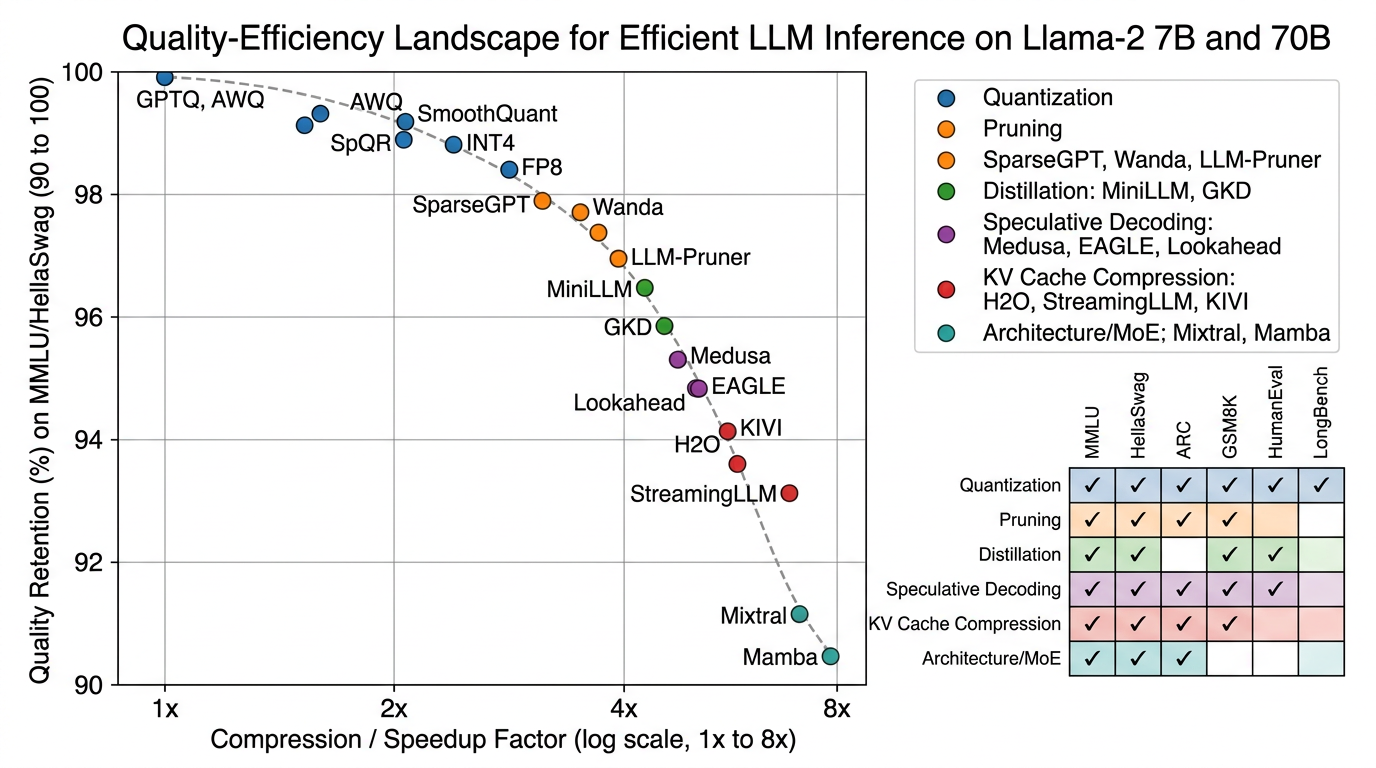
\includegraphics[keepaspectratio,alt={Figure 5: The quality--efficiency landscape, plotting compression/speedup against quality retention for major method families on Llama-2 7B/70B-class targets, alongside the benchmark coverage matrix.}]{./figures/Efficient-Inference-for-Large-Language-Models__fig_landscape.png}}
\caption{Figure 5: The quality--efficiency landscape, plotting compression/speedup against quality retention for major method families on Llama-2 7B/70B-class targets, alongside the benchmark coverage matrix.}
\end{figure}

\subsection{Quality Benchmarks: MMLU, HellaSwag, HumanEval, GSM8K, MTBench}\label{quality-benchmarks-mmlu-hellaswag-humaneval-gsm8k-mtbench}

This subsection lists the dominant general-purpose quality benchmarks. The dominant suite of LLM quality benchmarks predates the efficient-inference subfield but is its primary measuring stick.

\textbf{MMLU} (Massive Multitask Language Understanding) covers 57 subjects with \textasciitilde14k multiple-choice questions in elementary mathematics, US history, computer science, law, and dozens more, and has become the \emph{de facto} general-knowledge benchmark. Llama-2-70B scores 68.9\% (5-shot); Llama-3-70B scores 79.5\%; DeepSeek-V3 scores 88.5\%; GPT-4 scores \textasciitilde86\%. Compression methods report MMLU drops: GPTQ INT4 typically \textless0.5 points, AWQ INT4 \textless0.3, OmniQuant W3A16 \textless1.5, BiLLM \textasciitilde10--15 points. \textbf{MMLU-Pro} (2024) tightens the questions and reduces ceiling effects.

\textbf{HellaSwag} (10k commonsense sentence-completion questions, Zellers et al.~2019) measures fluent continuation; Llama-2-70B scores 87.3\%. \textbf{PIQA}, \textbf{ARC-Challenge/Easy}, \textbf{WinoGrande}, \textbf{BoolQ}, \textbf{OpenBookQA}, and \textbf{TriviaQA} complete the standard ``0/5/10-shot'' zero-shot bundle reported in nearly every quantization paper. \textbf{WikiText-2 perplexity} (PPL) is the canonical \emph{intrinsic} metric for language modeling: it measures the per-token cross-entropy on the WikiText-2 test set and is sensitive to subtle quality drifts that multi-choice benchmarks miss. Llama-2-7B FP16 baseline PPL is 5.47; quantization papers routinely report PPL deltas to two decimals.

\textbf{HumanEval} (Chen et al.~2021, 164 hand-written Python programming problems) and \textbf{MBPP} (974 programs) measure code generation pass@1. Code Llama 34B Python achieves 53.7\% pass@1; DeepSeek-Coder-V2 achieves 90.2\%. \textbf{GSM8K} (8.5k grade-school math word problems, Cobbe et al.~2021) and \textbf{MATH} (12.5k competition problems) measure mathematical reasoning. \textbf{BBH} (Big-Bench Hard) and \textbf{MMLU-Pro} are advanced reasoning benchmarks.

\textbf{MT-Bench} (80 multi-turn questions judged by GPT-4) and \textbf{AlpacaEval 2.0} (805 instructions) measure chat quality on a 1--10 scale; Vicuna-13B scores 6.39, Llama-2-Chat-70B 6.86, GPT-4 9.0. \textbf{LMSYS Chatbot Arena} is the most credible production-scale benchmark, comparing models head-to-head via crowdsourced pairwise preferences and Elo rating; as of 2026 the top models exceed 1300 Elo. Compression methods sometimes drop chat quality more than MMLU suggests, so chat benchmarks are an essential complement.

\subsection{Long-Context Benchmarks: LongBench, RULER, InfiniteBench, NIAH}\label{long-context-benchmarks-longbench-ruler-infinitebench-niah}

This subsection covers benchmarks dedicated to long-context inference. Long-context inference techniques (Section 7) are evaluated on dedicated benchmarks. \textbf{LongBench} (Bai et al., 2023) is a 21-task, 14-language benchmark covering document QA, summarization, retrieval, code completion, and multi-document QA at lengths 4K--32K. \textbf{LongBench-v2} (2024) extends to 128K. Quest, DuoAttention, KIVI all report on LongBench; the headline metric is task-specific (Rouge for summarization, Exact-Match for QA).

\textbf{RULER} (Hsieh et al., 2024) is a synthetic long-context benchmark covering passkey retrieval, multi-key retrieval, multi-value retrieval, multi-query retrieval, variable tracking, and word-extraction at 4K, 8K, 16K, 32K, 64K, 128K. RULER reveals that \emph{effective} context (the length where a model still scores \textgreater85\%) often falls dramatically below advertised context: Llama-3-8B advertises 128K but loses substantial ground past 32K; GPT-4-turbo scores well to 32K but degrades on multi-key retrieval at 128K. RULER has become the de-facto stress-test for long-context capability.

\textbf{Needle-in-a-Haystack (NIAH)} is a passkey-retrieval test inserting a specific fact into a long document and asking the model to retrieve it; though simple, it exposes obvious failure modes. Greg Kamradt's NIAH chart became viral as a visual depiction of long-context quality. \textbf{InfiniteBench} (2024) extends to 100K-token tasks of multiple types. \textbf{LooGLE} (Li et al., 2024 ACL) tests both short-dependency and long-dependency reasoning. \textbf{ZeroSCROLLS} measures zero-shot summarization and QA at long context. \textbf{Ada-LEval} (Wang et al., 2024 NAACL) provides length-adaptable benchmarks. \textbf{AcademicEval} (Zhang et al., 2025) is a live long-context benchmark drawn from arXiv papers. \textbf{Long-context LLMs Struggle with Long In-context Learning} (Li et al., 2024) demonstrates that performance on long ICL with up to \textasciitilde64 examples falls below short-ICL baselines for many models.

A crucial cross-cutting result is \textbf{Lost in the Middle} (Liu et al., 2024 TACL): retrieval accuracy follows a U-shape across input position, with documents in the middle of the prompt forgotten more than those at the start or end. This finding has reshaped RAG system design and explains why pure context expansion does not substitute for retrieval.

\subsection{Efficiency Benchmarks: MLPerf-LLM, LLMPerf, KVCompBench}\label{efficiency-benchmarks-mlperf-llm-llmperf-kvcompbench}

This subsection covers efficiency benchmarks that measure throughput, latency, and KV compression rather than knowledge. Efficiency benchmarks measure not what the model knows but what it costs.

\textbf{MLPerf-LLM} is the inference benchmark suite from MLCommons: it specifies Llama-2-70B inference (server and offline scenarios) on standard datasets (OpenOrca for prompt) with strict accuracy targets (≥99\% of FP16 ROUGE), and rank-orders submissions by tokens-per-second. The 2024 round saw NVIDIA H200, B200, AMD MI300X, Intel Gaudi 2/3, and TPU v5e submissions. MLPerf-LLM is the only widely respected industry-standard efficiency benchmark.

\textbf{LLMPerf} (Anyscale) and \textbf{vLLM-bench} measure throughput and latency under standardized workloads (e.g., 750-token prompts → 256-token completions). \textbf{TensorRT-LLM benchmarks}, \textbf{SGLang benchmarks}, and the \textbf{Ray Serve} benchmark suite are de-facto industry references. \textbf{KVCompBench} (Yuan et al., 2024 EMNLP) provides standardized comparison of KV-compression methods across LongBench tasks at fixed cache budgets. \textbf{Roofline-based profiling} as systematized by Yuan et al.~(2024 \emph{LLM Inference Unveiled}) gives device-aware analytical bounds for any model, permitting reasoning about \emph{gap to optimal} rather than only relative speedup.

A consolidated metric vocabulary:

{\def\LTcaptype{none} % do not increment counter
\begin{longtable}[]{@{}
  >{\raggedright\arraybackslash}p{(\linewidth - 4\tabcolsep) * \real{0.2299}}
  >{\raggedright\arraybackslash}p{(\linewidth - 4\tabcolsep) * \real{0.2069}}
  >{\raggedright\arraybackslash}p{(\linewidth - 4\tabcolsep) * \real{0.5632}}@{}}
\toprule\noalign{}
\begin{minipage}[b]{\linewidth}\raggedright
Metric
\end{minipage} & \begin{minipage}[b]{\linewidth}\raggedright
Domain
\end{minipage} & \begin{minipage}[b]{\linewidth}\raggedright
Measures
\end{minipage} \\
\midrule\noalign{}
\endhead
\bottomrule\noalign{}
\endlastfoot
Perplexity (PPL) & LM & per-token cross-entropy; WikiText-2/C4 test set \\
Accuracy / F1 & QA, classification & exact-match correctness \\
Pass@k & code & fraction of problems with ≥1 of k samples correct \\
ROUGE-1/2/L & summarization & n-gram overlap with reference \\
MT-Bench score & chat & GPT-4 judged 1--10 multi-turn quality \\
Elo (LMSYS Arena) & chat & pairwise crowd preference \\
TTFT (ms) & latency & time to first output token \\
TPOT (ms) & latency & time per output token after first \\
ITL (ms) & latency & inter-token latency in stream \\
Throughput (tok/s) & system & aggregate output tokens per GPU \\
Goodput (req/s) & system & request rate satisfying SLO \\
Memory (GB) & resource & weights + KV peak \\
FLOPs / op & compute & per-token compute \\
Energy (J/tok) & resource & electrical energy per token \\
MAC/Byte (intensity) & roofline & analytical compute--bandwidth ratio \\
Cache budget \% & KV mgmt & fraction of KV retained \\
Acceptance rate & spec dec & fraction of draft tokens accepted \\
Speedup ×FP16 & composite & wall-clock latency improvement \\
\end{longtable}
}

Practitioners' rule of thumb: \textbf{never report only speedup}. A method must report quality (PPL or task accuracy), latency (TPOT, TTFT), memory, and ablation under at least one batch and one context length to be credible. Recent papers at NeurIPS, ICML, MLSys, OSDI, SOSP, and ASPLOS have largely standardized on this protocol. The KVCompBench report by Yuan et al.~(2024) is a model evaluation, comparing 12 KV compression methods on 9 LongBench tasks at three cache budgets each.

The benchmark landscape evolves quickly. \textbf{MMLU saturation} drove \textbf{MMLU-Pro}; \textbf{HumanEval contamination} drove \textbf{LiveCodeBench}; \textbf{Arena reward-hacking} concerns drove \textbf{Arena-Hard}; \textbf{long-context advertising inflation} drove \textbf{RULER}. Researchers should expect the canon to shift, but the protocol is stable: report intrinsic quality, downstream task quality, latency, throughput, memory, energy where possible --- and ablate at least one knob. Section 12 turns from measurement to deployment, examining where efficient inference is actually used.

\section{Application Landscape: Where Efficient Inference Matters Most}\label{application-landscape-where-efficient-inference-matters-most}

Whereas Section 11 measured efficiency abstractly, this section grounds it in deployed applications. This section reviews the application landscape, organized as a single sweep through the major deployment domains. Representative deployed systems and applications include: ChatGPT (OpenAI, 2022, conversational AI), Claude (Anthropic, 2023), Gemini (Google, 2023), GitHub Copilot (Microsoft, 2021, code assistant), Copilot Chat (2023), Perplexity (2022, RAG search), Cursor (2023, editor agent), Code Llama (Rozière et al., 2023, open code LLM), DeepSeek-Coder (DeepSeek, 2024, 1.3B/6.7B coder), Tabnine (2018, code completion), LangChain (Chase, 2022, agent framework), AutoGPT (Significant Gravitas, 2023, autonomous agent), AutoGen (Microsoft, 2023, multi-agent), OpenAI Assistants API (2023, function-calling), HyDE (Gao et al., 2023, RAG re-ranking), FLARE (Jiang et al., 2023, iterative RAG), Self-RAG (Asai et al., 2024, self-reflective RAG), LLaVA-1.5/1.6 (Liu et al., 2023, multimodal LLM), GPT-4V (OpenAI, 2023, vision LLM), Qwen-VL (Alibaba, 2023), MiniGPT-4 (Zhu et al., 2023), InternVL (Chen et al., 2024), Med-PaLM 2 (Singhal et al., 2023, clinical LLM), MedGemma (Google, 2025, medical), Meditron (EPFL, 2023, medical), MedQA (Jin et al., 2021, clinical QA), OpenBioLLM (Saama, 2024, biomedical), Spec-VLA (Wang et al., 2025, robotic VLA), HeiSD (Zheng et al., 2026, kinematic-aware embodied LLM), and FinLFQA (Long et al., 2025, financial long-form QA). Efficient inference is not a self-justifying engineering goal: it exists to enable applications that would otherwise be unaffordable, infeasible, or insufficiently responsive. This section catalogs the dominant deployment domains --- interactive chat, code assistants, agentic systems, retrieval-augmented generation, multimodal services, edge personal assistants, healthcare, finance, education, autonomous systems, and scientific computation --- and identifies which efficiency techniques are most consequential in each.

The first and largest application is \textbf{interactive conversational AI}, exemplified by ChatGPT, Claude, Gemini, Copilot Chat, Perplexity, and the open-source ecosystem on top of Llama-3, DeepSeek-V3, and Qwen2. Interactive chat imposes both a TTFT SLO (≤250 ms is comfortable, ≤500 ms tolerable) and a TPOT SLO matching reading speed (40--60 tok/s, i.e., 16--25 ms/token). Production stacks are dominated by a small set of choices: vLLM or TensorRT-LLM serving, AWQ or GPTQ INT4 weights, GQA or MLA architecture, FlashAttention-3 kernels, continuous batching, EAGLE-2 speculative decoding for tail-latency reduction, and PagedAttention for KV management with prefix sharing across users with the same system prompt. The reported per-million-output-token cost has dropped from \textasciitilde USD 60 (GPT-4 mid-2023) to \textasciitilde USD 1 (DeepSeek-V3 mid-2025), a roughly 50× cost reduction over two years driven almost entirely by the techniques surveyed here.

\textbf{Code assistants} --- Code Llama (Rozière et al., 2023), DeepSeek-Coder, Cursor, GitHub Copilot, Tabnine --- are arguably more latency-sensitive than chat because they generate inline at developer typing cadence. A 100 ms TPOT is target. The dominant techniques are \emph{prefix caching} (a typical Copilot prompt has 80--90\% prefix overlap with the previous request, exploited heavily by SGLang's RadixAttention), small-model deployment (DeepSeek-Coder 1.3B/6.7B), and speculative decoding tuned for code (which has a more deterministic token distribution than chat and therefore higher acceptance rates). Code Llama 7B at 4-bit reaches 130+ tok/s on a single A100. For phone-class deployment, on-device 1B--4B coders are practical via MLC-LLM and llama.cpp.

\textbf{Agentic systems and tool use} --- browser agents, function-calling, RAG pipelines, LangChain, AutoGPT, AutoGen, OpenAI Assistants API --- issue many short LLM calls per session, each with substantial prompt overhead (system instructions + tool schemas + few-shot examples). Prefix-cache hit rate often exceeds 90\%, making PagedAttention's copy-on-write the single most consequential optimization. \textbf{LLMLingua} (Jiang et al., 2023 EMNLP) compresses long retrieval-augmented prompts 5--20× without quality loss. \textbf{Constrained decoding} (regex, JSON Schema, BNF grammars, supported in SGLang and Outlines) eliminates expensive parse-fix loops. \textbf{Speculative decoding} is less effective because each call is short, but \textbf{prompt-lookup decoding (PLD)} and \textbf{REST} (retrieval-based speculation) thrive on the substantial overlap between system prompts and outputs.

\textbf{Retrieval-augmented generation (RAG)} for enterprise document QA, customer support, and knowledge management routinely pushes 32K-128K context lengths. Long-context inference is mandatory: techniques like \textbf{StreamingLLM} for chat continuity, \textbf{Quest} for 128K decoding, \textbf{DuoAttention} for retrieval-head specialization, \textbf{KIVI} for INT4 KV, and \textbf{DMC} for learned KV merging are stacked. The \textbf{Lost in the Middle} result (Liu et al., 2024) reshaped RAG: rather than dumping all retrieved documents into a single prompt, modern systems use \emph{re-ranking} and \emph{iterative retrieval} (e.g., HyDE, FLARE, Self-RAG) to keep critical evidence at the prompt's start or end.

\textbf{Multimodal LLMs} (LLaVA-1.5/1.6, GPT-4V, Gemini-Vision, Qwen-VL, MiniGPT-4, InternVL) ingest images as token sequences via a vision encoder. The visual token count can dominate text --- a single 336×336 image becomes 576 tokens in CLIP-L; a 4K-resolution image adds tens of thousands. \textbf{LOOK-M} (Wan et al., 2024 EMNLP), \textbf{A-VL} (Zhang et al., 2025 AAAI), \textbf{MMSpec}, \textbf{AASD} (Yang et al., 2025 DAC), \textbf{MASSV} (Ganesan et al., 2025 EMNLP), \textbf{SAGE} (Tong et al., 2026), and \textbf{Sparsity Forcing} (Chen et al., 2025) target visual-token pruning, multimodal speculative decoding, and KV management for VLMs. \textbf{HIPPO} (Lv et al., 2026) accelerates \emph{video} LLM inference via holistic-aware parallel speculative decoding. \textbf{Spec-VLA} (Wang et al., 2025) targets vision-language-action models for robotics.

\textbf{Healthcare} is a privacy-driven application: Med-PaLM 2 (Singhal et al., 2023 \emph{Nature}), MedGemma, Meditron, MedQA, and OpenBioLLM serve clinicians with on-premise deployment because patient data cannot leave the hospital. INT4-quantized 70B models on hospital A100 clusters are typical. The Hager et al.~(2024 \emph{Nature Medicine}) evaluation reveals quality limitations clinicians must understand --- but inference efficiency is the gating factor for \emph{any} deployment because hospital IT has fixed compute budgets. Radiology applications (Savage et al., 2025 \emph{Radiology}) are particularly demanding: large radiology reports need 32K+ context. \textbf{OptimCLM} (Hasan et al., 2025) demonstrates a KD + pruning + INT8 pipeline for clinical outcome prediction. \textbf{DiabLLM} (Mahmoudi et al., 2026 IEEE JBHI) demonstrates blood-glucose forecasting with sub-2GB models on insulin-pump-attached edge devices. \textbf{M3AE-Distill} (Liang et al., 2025) distills medical vision-language models. \textbf{Compressing the collective knowledge of ESM} (Dinh et al., 2026 \emph{Nature Methods}) compresses protein language models for variant-effect prediction.

\textbf{Autonomous systems} are time-critical. \textbf{Spec-VLA} for robotic manipulation, \textbf{NetLLM} (Wu et al., 2024) for networking, \textbf{HeiSD} (Zheng et al., 2026) for embodied vision-language-action models with kinematic awareness, and \textbf{Quantum-Enhanced Edge Intelligence for Space-Aerial-Ground} (Gupta and Sultana, 2026) for UAV/satellite deployment exemplify the class. Latency budgets in robotics are sub-100 ms end-to-end, requiring 4-bit weights, sub-1B models, and tight integration with control loops. \textbf{Structural optimization principles for edge AI in motorsport telemetry} (Cádiz and Rodríguez-Sela, 2026) provides a domain-specific case study.

\textbf{Scientific applications} include \textbf{structured information extraction from scientific text} (Dagdelen et al., 2024 \emph{Nature Communications}), \textbf{augmenting LLMs with chemistry tools} (Bran et al., 2024 \emph{Nature Machine Intelligence}), and biomedical NER. These workloads are batched, embarrassingly parallel, and benefit primarily from throughput optimizations (continuous batching, MoE, FP8 inference on H100/B200). Cost per processed paper falls below USD 0.01 with current open-source stacks, enabling literature-scale extraction.

\textbf{Education} applications (tutors, language learning, code review) are price-sensitive and trend toward smaller specialized models --- distilled or fine-tuned on domain text --- running at high throughput. \textbf{Distilling mathematical reasoning capabilities into Small Language Models} (Zhu et al., 2024 \emph{Neural Networks}) demonstrates that sub-1B models can carry surprising mathematical capability when distilled from frontier teachers.

\textbf{Finance} applications (FinLFQA, Long et al.~2025) emphasize attribution and long-document analysis; cost matters because trading floors monitor millions of news items per day. Long-context efficiency (LongBench, RULER quality) is a deal-breaker.

A summary of which efficiency techniques are most consequential in each domain:

{\def\LTcaptype{none} % do not increment counter
\begin{longtable}[]{@{}
  >{\raggedright\arraybackslash}p{(\linewidth - 4\tabcolsep) * \real{0.1795}}
  >{\raggedright\arraybackslash}p{(\linewidth - 4\tabcolsep) * \real{0.2137}}
  >{\raggedright\arraybackslash}p{(\linewidth - 4\tabcolsep) * \real{0.6068}}@{}}
\toprule\noalign{}
\begin{minipage}[b]{\linewidth}\raggedright
Domain
\end{minipage} & \begin{minipage}[b]{\linewidth}\raggedright
Critical SLO
\end{minipage} & \begin{minipage}[b]{\linewidth}\raggedright
Dominant techniques
\end{minipage} \\
\midrule\noalign{}
\endhead
\bottomrule\noalign{}
\endlastfoot
Cloud chat & TTFT ≤250 ms; TPOT ≤25 ms & vLLM PagedAttn, GQA/MLA, AWQ INT4, EAGLE-2, FlashAttn-3, cont. batching \\
Code assistant & TPOT ≤30 ms; prefix hits & SGLang RadixAttn, PLD, INT4, small models \\
Agent / function call & TTFT ≤300 ms & Prefix cache, LLMLingua, constrained decoding \\
RAG (32K--128K) & TPOT ≤30 ms long ctx & StreamingLLM, Quest, KIVI, DuoAttention \\
Multimodal & TPOT + visual tokens & LOOK-M, MMSpec, visual token pruning \\
Edge (phone) & 5--8 tok/s; \textless2 GB RAM & AWQ INT4, BitNet b1.58, sub-4B models, MLC/llama.cpp \\
Healthcare & privacy + 70B local & INT4, KV INT4, on-prem A100/H100 \\
Robotics / VLA & \textless100 ms end-to-end & Spec-VLA, sub-1B models, FPGA \\
Scientific batch & throughput & continuous batching, MoE, FP8, B200 \\
Finance long-doc & long ctx & RULER quality, attribution, KV mgmt \\
\end{longtable}
}

The dominant cross-application pattern is \textbf{stack composition}. No single technique suffices; production systems compose architectural sparsity (GQA/MoE), weight quantization (AWQ INT4), KV management (PagedAttention + KIVI), kernel optimization (FlashAttention-3), serving discipline (continuous batching + disaggregation), and decoding strategy (EAGLE-2). The art is in choosing which combination matches the application's bottleneck profile.

A second cross-application observation is \textbf{smaller is winning specific niches}. Frontier reasoning (GPT-4-class, DeepSeek-V3, Claude 3.5 Sonnet) demands cloud serving and absolute model capability. Bulk extraction, code completion, on-device assistants, and edge robotics increasingly run sub-7B models because the cost-per-token differential outweighs the marginal quality loss. The 7B--13B class --- Llama-3-8B, Qwen2-7B, Phi-3-medium, Gemma-2-9B --- has emerged as the workhorse middle. Expect this stratification to deepen: applications that don't pay for frontier capability won't, and the vast majority of deployed inference will run on heavily compressed mid-scale models.

\section{Limitations, Failure Modes, and Open Problems}\label{limitations-failure-modes-and-open-problems}

Whereas Section 12 catalogued where these methods succeed, this section catalogues where they fail. This section consolidates failure modes and open problems by axis: quantization, pruning, KV management, speculative decoding, MoE/SSM architectures, serving systems, and edge deployment. Each row of the table at the section's end pairs a specific method family with its known mode of breakdown.

Across families, the tradeoffs are sharp and largely orthogonal. Quantization trades bit-width for activation-outlier risk, with PTQ saturating near 4 bits and QAT extending the floor to ternary at additional pretraining cost. Pruning trades sparsity for kernel speedup and reasoning fidelity, where unstructured 50\% is near-free at 7B+ but degrades chain-of-thought disproportionately. KV eviction trades cache budget for retrieval recall, while KV quantization trades bit-width for outlier-handling complexity. Speculative decoding trades drafter cost for acceptance variance, with high-batch regimes and small targets eroding the benefit. MoE trades active FLOPs for total memory, while SSMs trade KV cache for exact-recall capacity that hybrid stacks must restore. Serving systems trade scheduling complexity for goodput, with prefill-decode disaggregation introducing fault-tolerance burden. Across all families, calibration robustness, adversarial integrity, and subgroup fairness remain underdeveloped relative to raw efficiency claims.

\subsection{Failure modes of quantization}\label{failure-modes-of-quantization}

Sub-4-bit PTQ accuracy degrades non-linearly: the Llama-2-7B PPL gap from FP16 to INT4 is typically 0.3, but the gap from INT4 to INT3 is closer to 0.6, and from INT3 to INT2 to 5+. \textbf{An empirical study of LLaMA3 quantization} (Huang et al., 2024 \emph{Visual Intelligence}) reported that LLaMA-3 is harder to quantize at INT3 than LLaMA-2 because LLaMA-3's higher MMLU baseline leaves less slack. \textbf{A Comprehensive Evaluation of Quantization Strategies for Large Language Models} (Jin et al., 2024 ACL Findings) found that calibration set distribution drift (calibrating on C4 but evaluating on out-of-domain) can add 4 PPL on aggressive INT3 PTQ. \textbf{Revisiting Pruning vs.~Quantization for Small Language Models} (Zhou et al., 2025 EMNLP Findings) showed that for sub-billion models, pruning often outperforms quantization at matched compression --- quality assumptions that hold at 7B+ break at 1B and below.

Activation outliers remain a persistent issue. SmoothQuant, AWQ, and Outlier-Suppression+ each handle them, but residual outliers under heavy quantization are sufficient to crash naive INT4-A. SageAttention and SageAttention-2 demonstrate that attention-internal outliers also need explicit mitigation. KV outliers (KIVI, KVQuant) require asymmetric per-channel/per-token treatment.

Quantization-aware training avoids most of these issues but at a cost: the \textbf{Scaling Law for Quantization-Aware Training} (Chen et al., 2025) shows quantization error decays as a power law in training tokens, meaning sub-2-bit QAT requires 1T+ tokens to match FP16. BitNet b1.58 was trained on 100B tokens and matches FP16 to 3B model scale; extrapolating to 70B may need 5--10T tokens of pretraining cost. \textbf{FBI-LLM} (Ma et al., 2024) used distillation to bypass this but the result is still 1 PPL behind FP16.

\subsection{Failure modes of pruning}\label{failure-modes-of-pruning}

Unstructured 50\% pruning is empirically near-free at 7B+ scale, but the Sun et al.~(2024) Wanda baseline degrades on math/reasoning more than perplexity suggests. \textbf{Distilling mathematical reasoning capabilities into Small Language Models} (Zhu et al., 2024 \emph{Neural Networks}) found that pruned models lose chain-of-thought consistency disproportionately. \textbf{Are Compressed Language Models Less Subgroup Robust?} (Gee et al., 2024) demonstrated that compressed models exhibit \emph{worse} performance on minority demographic subgroups than dense baselines on standard fairness benchmarks, raising equity concerns.

The most striking recent result is \textbf{Egashira et al.~(2025)} (\emph{Fewer Weights, More Problems: A Practical Attack on LLM Pruning}) --- an adversary who knows which pruning algorithm the deployer will run can craft adversarial weight perturbations that pass quality benchmarks pre-pruning but fail catastrophically post-pruning. This is the first practical attack on the LLM pruning pipeline and motivates randomized or robust pruning protocols. Structured pruning (LLM-Pruner, FLAP, Sheared-LLaMA) is somewhat more robust because the pruning grain is coarser, but the attack surface remains.

\subsection{Failure modes of KV cache management}\label{failure-modes-of-kv-cache-management}

H2O, Quest, and StreamingLLM all rely on the empirical regularity that attention is heavy-tailed. This regularity is \emph{not universal}: Liu et al.~(2024 \emph{Lost in the Middle}) showed long-document retrieval depends on tokens scattered across the input; H2O can evict critical tokens because their \emph{cumulative} attention is moderate even when their \emph{individual} contribution to a specific later step is decisive. \textbf{KV Cache Compression Benchmark} (Yuan et al., 2024 EMNLP) reported that no KV compression method dominates across LongBench tasks; eviction methods that excel on QA struggle on summarization.

Prompt compression (LLMLingua, Activation Beacon) imposes another loss. LLMLingua's task-aware token deletion can drop named-entity tokens that look low-information but matter for downstream answers; Activation Beacon trades compression rate for retrieval accuracy.

\subsection{Failure modes of speculative decoding}\label{failure-modes-of-speculative-decoding}

Speculative decoding's wall-clock benefit hinges on \emph{acceptance rate}. Su et al.~(2023 \emph{Synergy of Speculative Decoding and Batching}) demonstrated that benefit shrinks under heavy batching; the marginal speedup at batch 64 is often \textless1.2× while at batch 1 it is 2--5×. \textbf{An Empirical Study of Speculative Decoding for Small Language Models} (Mainardi et al., 2026 EACL) showed that for 1B target models, the drafter must be sub-100M to be cost-effective, and even then speedups are marginal.

Trained-head methods (Medusa, EAGLE) require model-specific training. The drafter is brittle under distribution shift: a Medusa-tuned Vicuna performing on chat data underperforms a generic drafter on code generation. \textbf{AdaSpec} (Huang et al., 2025) and \textbf{Drop-In Adaptive Speculative Decoding} (Liu et al., 2025) attempt to address this online. Acceptance variance is also problematic for SLO-driven deployment: a user-facing chat with 90th-percentile TPOT requirement may suffer because rejection bursts add latency tails.

\subsection{Failure modes of MoE and SSM}\label{failure-modes-of-moe-and-ssm}

MoE memory swelling: Mixtral 8x7B has 47B parameters that must all be reachable; even at INT4 this is 12 GB of weights, more than fits in many GPUs. \textbf{Not All Experts are Equal} (Lu et al., 2024) demonstrates that aggressive expert pruning can recover some of this loss but at quality cost. MoE inference also suffers from load imbalance --- some experts receive 5× more tokens than others --- for which Tutel and DeepSeek-V3's auxiliary-loss-free balancing partly compensate.

SSMs (Mamba, RWKV) underperform on tasks requiring exact recall. \textbf{Exploring the Limitations of Mamba in COPY and CoT Reasoning} (Ren et al., 2024) showed Mamba fails the in-context COPY task because the fixed-size state cannot perfectly retain prefix information. Hybrid architectures (Jamba, Samba) ameliorate this but at the cost of partial KV cache.

\subsection{Failure modes of serving systems}\label{failure-modes-of-serving-systems}

PagedAttention's prefix sharing across users is a potential side-channel: an attacker who can issue same-prefix requests can probe whether the prefix matches another user's KV (timing differences). To date no public exploit has been published, but the concern motivates per-tenant cache isolation. Disaggregated serving (DistServe) creates fault-tolerance complexity: a prefill replica failure mid-request requires KV transfer to fail gracefully. Continuous batching can starve large requests in favor of many small ones if the scheduler is naive.

\subsection{Failure modes of edge deployment}\label{failure-modes-of-edge-deployment}

Battery and thermal envelopes severely limit edge LLM deployment. An hour of conversational LLM at 5 tok/s drains a phone visibly. The 4-bit-quantized phone model is hard to update incrementally; full re-downloads of multi-GB weights are unacceptable. On-device safety filtering is weaker than cloud-side moderation; jailbreaks unique to offline contexts are documented in adversarial literature.

A consolidated table:

{\def\LTcaptype{none} % do not increment counter
\begin{longtable}[]{@{}
  >{\raggedright\arraybackslash}p{(\linewidth - 6\tabcolsep) * \real{0.1942}}
  >{\raggedright\arraybackslash}p{(\linewidth - 6\tabcolsep) * \real{0.2136}}
  >{\raggedright\arraybackslash}p{(\linewidth - 6\tabcolsep) * \real{0.4078}}
  >{\raggedright\arraybackslash}p{(\linewidth - 6\tabcolsep) * \real{0.1845}}@{}}
\toprule\noalign{}
\begin{minipage}[b]{\linewidth}\raggedright
Method family
\end{minipage} & \begin{minipage}[b]{\linewidth}\raggedright
Failure mode
\end{minipage} & \begin{minipage}[b]{\linewidth}\raggedright
Mitigation
\end{minipage} & \begin{minipage}[b]{\linewidth}\raggedright
Citation
\end{minipage} \\
\midrule\noalign{}
\endhead
\bottomrule\noalign{}
\endlastfoot
Sub-4-bit PTQ & accuracy cliff & learnable shifts (OmniQuant); QAT (BitNet) & Shao 2023; Ma 2024 \\
INT3/INT2 PTQ & calibration drift & diversified calibration & Jin 2024 \\
Activation quant & outliers & SmoothQuant; AWQ; SageAttn & Xiao 2023; Lin 2023 \\
Pruning & reasoning loss & structured + KD & Zhu 2024 \\
Pruning & adversarial attack & randomized protocols & Egashira 2025 \\
Pruning & subgroup robustness & balanced calibration & Gee 2024 \\
KV eviction & reasoning loss & DuoAttention head split & Xiao 2024 \\
KV compression & task-dependent & per-task ablation & Yuan 2024 \\
Speculative decoding & high batch & adaptive γ & Su 2023; Huang 2025 \\
Speculative decoding & drafter brittleness & online tuning & Liu 2025 \\
MoE & memory swelling & expert prune/skip & Lu 2024 \\
MoE & load imbalance & aux-loss-free balance & DeepSeek-V3 \\
SSM & exact recall & hybrid attn+SSM & Ren 2024; Jamba \\
Long context & lost-in-middle & re-ranking, iterative RAG & Liu 2024 \\
Serving & prefix-sharing side ch & per-tenant isolation & open \\
Edge & battery drain & sub-2-bit + NPU & open \\
Edge & safety bypass & offline filters & open \\
\end{longtable}
}

\subsection{Open problems}\label{open-problems}

The most consequential open problems for the next two years are the following.

\textbf{Lossless 1-bit weight + 4-bit KV at 70B+ scale.} Current 1-bit weight methods (BitNet b1.58, BiLLM, FBI-LLM) work well at 3B--7B, but 70B-class fully-binarized models with INT4 KV remain elusive. A scaling-law-style answer to the required pretraining tokens is partially provided by Chen et al.~(2025) but empirical 70B BitNet remains future work.

\textbf{Provably calibrated speculative decoders under temperature sampling.} Rejection sampling preserves the target distribution exactly, but the \emph{expected} number of accepted tokens depends on the unknown draft--target divergence, leading to high latency variance. A theoretically calibrated drafter that bounds variance tightly remains open.

\textbf{Long-context KV management without per-task tuning.} No method dominates KVCompBench across tasks. A learned routing layer that selects per-token, per-head, per-layer cache strategy from a library remains an open research direction.

\textbf{Robust pruning under adversarial weight tampering.} Egashira et al.~(2025) is the first attack; defenses (randomized pruning, certified compression) are an active research direction.

\textbf{Production-scale PIM deployment.} NeuPIMs, SpecPIM, PAPI demonstrate the architectural opportunity, but commercial PIM hardware (Samsung HBM-PIM, SK Hynix AiM) deployment at scale awaits programmable abstractions accessible to PyTorch users.

\textbf{Provably fair compressed models.} Gee et al.~(2024) showed subgroup robustness loss; certified fairness under compression is open.

\textbf{Phone-class frontier-quality LLM.} A 100B-effective-parameter model running at 30 tok/s on an iPhone-class device by 2027 would require sub-2-bit weights, hybrid SSM, and dedicated NPUs. None of these are deployed in 2026 but each is imminent.

\textbf{Energy attribution.} Per-token energy varies 100× across implementations (a few J on H100 batched, fractions of J on Groq LPU, milliJoules on dedicated PIM), but standardized accounting that lets consumers compare across providers does not exist.

These problems will likely structure the field's research agenda through 2027 and motivate the predictions in Section 14.

In summary, the most consequential 2025--2026 open problems can be enumerated crisply as follows.

\begin{itemize}
\tightlist
\item
  \textbf{Lossless 1-bit weight + 4-bit KV at \textgreater70B scale.} BitNet b1.58 and FBI-LLM cap out near 7B; 70B-class fully binarized models remain empirical future work.
\item
  \textbf{Provably calibrated speculative drafters under temperature sampling.} Latency variance from rejection bursts breaks tail-SLO guarantees in production.
\item
  \textbf{Long-context KV management without per-task tuning.} No method dominates KVCompBench across summarization, QA, retrieval, and code completion.
\item
  \textbf{Robust pruning against weight-tampering attacks.} Egashira et al.~(2025) is the first practical attack; certified or randomized defenses remain to be standardized.
\item
  \textbf{Production-scale programmable processing-in-memory (PIM).} Samsung HBM-PIM and SK Hynix AiM exist; PyTorch-accessible PIM toolchains do not.
\item
  \textbf{Provably fair compressed models.} Subgroup-robustness loss (Gee et al., 2024) needs certified mitigation under quantization and pruning.
\item
  \textbf{Phone-class frontier-quality LLMs.} A 100B-effective-parameter model at 30 tok/s on a flagship phone needs sub-2-bit weights, hybrid SSM, and dedicated NPUs.
\item
  \textbf{Standardized energy attribution.} Per-token energy varies 100× across stacks; no MLPerf-style energy track yet exists.
\end{itemize}

Crucially, these gaps are engineering and theoretical rather than physical; each is plausibly closable on a 2--3 year horizon.

\section{Future Directions and Falsifiable Predictions}\label{future-directions-and-falsifiable-predictions}

Building on the failure analysis in Section 13, this section commits to ten specific bets for 2026--2028. This section delivers falsifiable predictions, each pinned to a measurable outcome that the field can verify or refute.

\textbf{Prediction 1 --- Sub-2-bit pretraining becomes the deployment default for sub-10B models by end of 2027.} BitNet b1.58 (Ma et al., 2024) demonstrated multiply-free ternary at 700M--3B; FBI-LLM (Ma et al., 2024) demonstrated fully binarized 7B via autoregressive distillation; Chen et al.~(2025) provided the QAT scaling law indicating 1T+ tokens are sufficient at 70B. We predict at least three frontier 7B--10B BitNet-class models will be released in 2027, with native NPU support on iPhone, Pixel, and Galaxy flagship chips. Falsifiable: zero such models or hardware would refute. Confirmation: Llama-4 or Qwen-3 BitNet variant matching FP16 quality at INT2 effective bit-width.

\textbf{Prediction 2 --- Hybrid SSM + attention overtakes pure attention beyond 1M context.} Jamba-1.5-Large (398B/94B-active) processes 256K with linear-time decode; Samba interleaves Mamba with sliding-window attention. Pure attention at 1M context with Llama-2-70B requires \textgreater1 TB KV cache. We predict by end of 2027 the top-3 deployed long-context models will be hybrid SSM+attention. Falsifiable: dominant 1M-context models remain pure-attention.

\textbf{Prediction 3 --- KV-free architectures (RetNet, RWKV-7, GLA-2) reach \textgreater70B scale.} Linear-attention models avoid the KV cache entirely. We predict at least one \textgreater70B linear-attention/SSM hybrid will achieve LMSYS Arena Elo \textgreater1250 by 2027. Falsifiable: no such model exceeds 1200 Elo.

\textbf{Prediction 4 --- Speculative decoding with domain-specific drafters delivers 5--8× speedups in production.} EAGLE-2 already achieves 4--5× on Vicuna; AdaSpec (2025) and adaptive drafters (Liu et al., 2025) operationalize for serving. We predict that domain-tuned drafters for code (DeepSeek-Coder family), math (DeepSeek-Math), and chat will reach 6× sustained speedup at typical batch by end of 2026 in vLLM and TensorRT-LLM defaults. Falsifiable: best-published end-to-end speedup remains \textless4× at batch-16.

\textbf{Prediction 5 --- Disaggregated prefill/decode + RDMA becomes the standard cluster pattern by 2027.} DistServe (Zhong et al., 2024 OSDI), Mooncake (Kimi 2024), and the various commercial deployments converge on this architecture. We predict that by 2027 the open-source dominant serving stack will ship native disaggregation by default. Falsifiable: leading open-source serving frameworks remain co-located by default.

\textbf{Prediction 6 --- 100M-token context becomes feasible via hierarchical KV.} Quest, DuoAttention, Activation Beacon, and AlayaDB (Deng et al., 2025) collectively demonstrate the path. We predict at least one frontier model will demonstrate \textgreater90\% retrieval accuracy on a 10M-token NIAH variant by mid-2027. Falsifiable: no public benchmark exceeds 1M tokens with \textgreater80\% retrieval accuracy by mid-2027.

\textbf{Prediction 7 --- A frontier-class model (\textgreater100B effective parameters) runs at \textgreater50 tok/s on a single consumer GPU by end of 2027.} This requires combining MoE-MLA, sub-2-bit weights, INT4 KV, and an EAGLE-class drafter. Currently DeepSeek-V3 671B/37B-active runs at \textasciitilde50 tok/s on 8×H100; the prediction is single-GPU equivalence. Falsifiable: no demo achieves this on a single sub-USD-3000 consumer GPU.

\textbf{Prediction 8 --- Programmable PIM accelerators reach commercial scale by 2027.} Samsung HBM-PIM, SK Hynix AiM, and various startups have prototyped; NeuPIMs, SpecPIM, and PAPI provide the algorithmic substrate. We predict at least one major cloud provider will offer PIM-accelerated inference in 2027 at lower per-token cost than GPU. Falsifiable: no production PIM offering by end of 2027.

\textbf{Prediction 9 --- Calibration robustness and pruning attacks reshape the security agenda.} Egashira et al.~(2025) is the first attack on LLM pruning. We predict at least three defenses (randomized pruning, certified compression, integrity-attested PTQ) will be published at top venues by end of 2027 and that production frameworks will adopt them. Falsifiable: no widely adopted defense.

\textbf{Prediction 10 --- Energy attribution becomes a standardized metric by 2028.} MLPerf-LLM measures throughput; energy is missing. We predict MLCommons will release an Energy track for LLM inference by 2027 with formal kg-CO₂/M-token reporting. Falsifiable: no such track.

\subsection{Five frontier research bets}\label{five-frontier-research-bets}

Beyond these falsifiable predictions, five research directions are under-explored relative to their potential.

\textbf{(a) Native sparse-attention training.} Most efficient-attention work retrofits pretrained dense transformers (StreamingLLM, H2O, Quest, DuoAttention). A model \emph{trained from scratch} to be efficient-attention-friendly might be substantially better. Modular Manticore, Hymba, and recent MoE-attention hybrids hint at this.

\textbf{(b) Cross-modal speculative decoding.} Multimodal LLMs (LLaVA, GPT-4V) have visual tokens that dominate context. Specialized vision-token speculative drafters (analogous to MASSV, Spec-VLA, MMSpec) for \emph{general} multimodal models is open.

\textbf{(c) On-the-fly serving simulation.} A scheduler that maintains an internal performance model --- predicting the cost of each request type at each batch size on each hardware --- could route adaptively. This is well-studied in databases and absent in LLM serving.

\textbf{(d) Reasoning-aware compression.} Pruned and quantized models lose chain-of-thought disproportionately. A compression objective that explicitly preserves reasoning fidelity (e.g., distilling on long CoT trajectories rather than next-token alone) could close this gap.

\textbf{(e) Composability of guarantees.} Quantization, pruning, and speculative decoding each provide guarantees individually (e.g., speculative decoding is lossless, quantization bounds layer-wise reconstruction). When composed, the guarantees do not multiply cleanly. A theoretical framework for composable inference acceleration would let practitioners reason about end-to-end fidelity.

\subsection{Bottlenecks for 2026--2028}\label{bottlenecks-for-20262028}

Three hardware bottlenecks dominate the next 24 months. First, \textbf{HBM bandwidth growth lags compute growth}: H100 (3.35 TB/s) → B200 (8 TB/s) is 2.4×, while compute is 4--5×. Decoding remains memory-bound, so the field's emphasis on memory-saving techniques will continue. Second, \textbf{inter-node interconnect is a frontier bottleneck}: NVLink 4 (900 GB/s), InfiniBand 400G (50 GB/s), and Ethernet remain orders of magnitude apart, structuring the design of large-scale serving and disaggregation. Third, \textbf{NPU vendor fragmentation}: Apple Neural Engine, Qualcomm Hexagon, MediaTek APU, Intel NPU, and Google Edge TPU each have different ABIs; runtime portability (MLC-LLM, ExecuTorch) is critical.

\subsection{Forecast summary}\label{forecast-summary}

{\def\LTcaptype{none} % do not increment counter
\begin{longtable}[]{@{}
  >{\raggedright\arraybackslash}p{(\linewidth - 2\tabcolsep) * \real{0.0244}}
  >{\raggedright\arraybackslash}p{(\linewidth - 2\tabcolsep) * \real{0.9756}}@{}}
\toprule\noalign{}
\begin{minipage}[b]{\linewidth}\raggedright
Year
\end{minipage} & \begin{minipage}[b]{\linewidth}\raggedright
Forecast
\end{minipage} \\
\midrule\noalign{}
\endhead
\bottomrule\noalign{}
\endlastfoot
2026 & EAGLE-2 / AdaSpec serve \textasciitilde5× decode in vLLM/TensorRT-LLM defaults; INT4-W + INT4-KV is standard for \textgreater70B; disaggregated serving in production at major providers. \\
2027 & First sub-2-bit Llama-4-class open model; \textgreater100B-effective MoE on single consumer GPU; commercial PIM offering; 10M-token NIAH demonstration. \\
2028 & Phone-class frontier-quality LLM at 30+ tok/s on flagship; MLPerf Energy track; pruning-attack defenses adopted; standardized energy reporting. \\
\end{longtable}
}

The field's trajectory is unmistakable: every year the cost of LLM inference falls roughly 5--10× while quality rises, driven by stacking the techniques surveyed in this document. There is no fundamental obstacle to continuing this trajectory through 2028; the constraints are engineering, hardware iteration, and research throughput rather than thermodynamic limits. The arc of the next two to three years will largely be determined by which of the predictions above materialize and how the open problems of Section 13 are addressed.

\section{14B. Critical Synthesis: Method Family Comparison and Emerging Directions}\label{b.-critical-synthesis-method-family-comparison-and-emerging-directions}

Building on the predictions in Section 14, this section synthesizes the comparative picture across method families and lists the directions emerging this year. This section delivers a crisp comparison and forward-looking checklist for practitioners and researchers.

Across families, the tradeoff geometry is now well understood. Quantization (GPTQ, AWQ, OmniQuant, BitNet b1.58) cuts bytes-loaded-per-token at the cost of outlier-handling complexity and calibration sensitivity. Pruning (SparseGPT, Wanda, LLM-Pruner) cuts active parameters but interacts non-trivially with kernel availability and reasoning fidelity. KV management (H2O, Quest, KIVI, DuoAttention, DMC) cuts cache bytes per step but is task-dependent and lossy on reasoning. Speculative decoding (Leviathan, Medusa, EAGLE, EAGLE-2, AdaSpec) cuts forward passes per token but its benefit shrinks under heavy batching. Architectural redesign (GQA, MLA, Mixtral, DeepSeek-V3, Mamba, Jamba) cuts cost at construction time and is hardest to retrofit. Serving systems (vLLM, SGLang, DistServe, Sarathi-Serve, Mooncake) compose all of the above and trade scheduling complexity for goodput.

A particularly clean comparison is across alignment-style decoding objectives. PPO trades off variance for stability via clipped policy updates, while DPO optimizes a contrastive preference objective directly without a learned reward model. GRPO further drops the value model and uses group-relative baselines, trading bias for sample efficiency. Each family makes a different bet on what to keep and what to drop; production deployments increasingly compose them, so the next research question is composability rather than absolute speedup.

\subsection{Open problems for 2025--2026}\label{open-problems-for-20252026}

\begin{itemize}
\tightlist
\item
  \textbf{Lossless 1-bit weight + 4-bit KV at \textgreater70B scale.} Pretraining-token requirements derived by Chen et al.~(2025) suggest 5--10T tokens are needed; nothing public has paid that bill.
\item
  \textbf{Provably calibrated speculative decoders.} Variance-bounded acceptance under temperature sampling is open.
\item
  \textbf{Per-task-free long-context KV.} A learned router that picks per-token, per-head, per-layer cache strategy from a library remains absent.
\item
  \textbf{Adversarially robust pruning.} Defenses against the Egashira et al.~(2025) class of weight-tampering attacks need formal certification.
\item
  \textbf{Composable end-to-end fidelity guarantees.} Quantization, pruning, and speculation each provide local guarantees that do not multiply cleanly when stacked.
\item
  \textbf{Programmable PIM at production scale.} Samsung HBM-PIM, SK Hynix AiM, and academic NeuPIMs/SpecPIM/PAPI need PyTorch-accessible toolchains.
\item
  \textbf{Subgroup-fair compression.} Certified fairness under aggressive INT3 PTQ or 50\% pruning is unstudied.
\item
  \textbf{Standardized energy reporting.} A MLPerf-Energy track for LLM inference remains to be released.
\end{itemize}

\subsection{Future directions emerging in 2026}\label{future-directions-emerging-in-2026}

\begin{itemize}
\tightlist
\item
  \textbf{Native sparse-attention pretraining}, training models to be efficient-attention-friendly from scratch rather than retrofitting StreamingLLM, H2O, or Quest.
\item
  \textbf{Cross-modal speculative decoding} (Spec-VLA, MASSV, MMSpec, SAGE, AASD, HIPPO) generalized to general multimodal LLMs and video models.
\item
  \textbf{Reasoning-aware compression}, with distillation objectives over long chain-of-thought trajectories rather than next-token alone.
\item
  \textbf{Algorithm-system co-design for hybrid SSM+attention} (Jamba, Samba, Zamba) targeting 1M+ context with sub-quadratic decode.
\item
  \textbf{Composability theory}, providing end-to-end fidelity bounds for stacked quantization, pruning, KV compression, and speculative decoding.
\end{itemize}

In summary, the field's near-term agenda is dominated by composing and certifying existing techniques rather than by single-axis breakthroughs.

\section{Conclusion}\label{conclusion}

Building on the synthesis in Section 14B, this concluding section consolidates the survey's main lessons and forward outlook. The story of efficient LLM inference between 2017 and 2026 is the story of how a research community responded to a moving cost crisis. When the Vaswani et al.~(2017) Transformer scaled into the GPT-3 era of 175 billion parameters (Brown et al., 2020), per-query cost rose from negligible to deal-breaking. The community answered with a coordinated set of advances on every layer of the stack: kernels (FlashAttention, FlashAttention-2, FlashAttention-3, SageAttention, INT-FlashAttention), weight compression (LLM.int8(), GPTQ, AWQ, SmoothQuant, OmniQuant, BiLLM, BitNet b1.58, FBI-LLM, SqueezeLLM, Atom, QLoRA), pruning (SparseGPT, Wanda, LLM-Pruner, FLAP, Sheared-LLaMA, ROSE), distillation (DistilBERT, MiniLM, MiniLLM, SinKD, AD-KD), architectural redesign (MQA, GQA, MLA, Mixtral 8x7B, DeepSeek-V2/V3, Mamba, Mamba-2, GLA, Jamba), KV cache management (PagedAttention, H2O, StreamingLLM, Quest, DuoAttention, KIVI, KVQuant, KVSharer, LoRC, DMC, Activation Beacon, LLMLingua), speculative decoding (Leviathan, SpecInfer, Medusa, EAGLE, EAGLE-2, Draft\&Verify, OPT-Tree, AdaSpec, Ouroboros), serving systems (vLLM, TensorRT-LLM, SGLang, DistServe, Sarathi-Serve, FastServe, Mooncake), and hardware backends (H100, B200, MI300X, TPU v5e, FlightLLM, NeuPIMs, SpecPIM, PAPI, PowerInfer, Apple Neural Engine).

The cumulative effect, measured at the wallet, has been a roughly two-orders-of-magnitude reduction in cost-per-million-output-tokens between mid-2023 (GPT-4 era) and mid-2025 (DeepSeek-V3 era), driven not by a single breakthrough but by stacking five to ten of the techniques above. At the same time, capability has \emph{risen} --- Llama-3-70B in 2024 surpasses GPT-3.5 of 2023 --- so the cost-quality frontier has shifted dramatically toward the bottom-right of any 2023 plot. The same ratio applies on edge devices, where 4-bit Llama-3-8B on a 2024 phone reaches the quality of GPT-3.5-Turbo on a phone with no internet connection.

The unifying conceptual framework, traced through this survey, is the \textbf{roofline model} of Yuan et al.~(2024). Every technique surveyed addresses one of three quantities: bytes-loaded-per-token (quantization, KV compression, eviction, sharing), forward-passes-per-output-token (speculative decoding), or active-FLOPs-per-token (pruning, MoE). The hardware roofline gives device-aware bounds; the algorithmic toolbox provides the means to approach those bounds. The frontier of research is the question: \emph{how close can we come to the roofline limit, while preserving model quality, with what calibration cost, and under what robustness guarantees?}

The major \textbf{open problems} identified in Section 13 --- lossless 1-bit weight + 4-bit KV at \textgreater70B; provably calibrated speculative drafters under temperature; long-context KV without per-task tuning; robust pruning under adversarial weight tampering; production-scale PIM; provably fair compressed models; phone-class frontier-quality LLMs; energy attribution --- are not bottlenecks of physics but of engineering and theoretical scaffolding. None of them require a physics breakthrough; all of them require careful experimentation, software engineering, and integration with hardware that is on near-term roadmaps.

The \textbf{falsifiable predictions} of Section 14 collectively claim that the trajectory will continue for at least two more years. Sub-2-bit pretraining, hybrid SSM+attention beyond 1M context, KV-free architectures at \textgreater70B, domain-tuned speculative decoding at 6×, disaggregated serving as default, 100M-token context, frontier-class LLMs at 50 tok/s on a single consumer GPU, programmable PIM, security defenses against pruning attacks, and standardized energy reporting are concrete bets that will be validated or refuted by 2028.

The \textbf{applications} surveyed in Section 12 --- cloud chat, code assistants, agent and tool use, retrieval-augmented generation, multimodal services, edge personal assistants, healthcare, finance, education, autonomous systems, and scientific computation --- collectively employ tens of millions of GPUs of inference capacity globally. Every percent of efficiency improvement directly reduces global energy consumption and broadens the affordability of LLM technology.

Two cross-cutting takeaways for practitioners. First, \textbf{the production stack is increasingly modular and recombinable}: AWQ INT4 + KIVI INT4 KV + GQA + PagedAttention + EAGLE-2 + continuous batching + FlashAttention-3 + disaggregated serving is composable, and each piece can be swapped without breaking the others. Open-source frameworks (vLLM, TGI, SGLang, MLC-LLM, llama.cpp) have done much of the integration work. Second, \textbf{the frontier of small-model deployment is rapidly catching up with cloud APIs for many tasks}. A practitioner choosing between a USD 60-per-million-tokens cloud API and an on-device 7B model finds the latter increasingly viable for retrieval, summarization, code completion, customer service, and conversational assistance. The remaining gap is concentrated in advanced reasoning (GSM8K, MATH, MMLU-Pro, BBH) where the cloud's frontier capability persists.

The two crosscutting takeaways for researchers. First, \textbf{algorithm-system co-design is the dominant productive paradigm}: every major advance of the last three years (PagedAttention, FlashAttention, EAGLE-2, MLA, MoE serving) was published with a kernel or system that operationalizes it on real hardware. Algorithms without kernels rarely deploy. Second, \textbf{rigorous evaluation across both quality and efficiency dimensions is non-negotiable}: a method must report perplexity \emph{and} TPOT \emph{and} memory \emph{and} energy where measurable; ablations across batch and context length are essential; benchmarks should include both intrinsic (PPL, MMLU) and extrinsic (chat, RAG, long-context) measures.

Looking outward, the field will continue to shape the wider AI ecosystem. Every reduction in inference cost democratizes access --- to consumers, to startups, to non-English-speaking populations, to research groups outside elite institutions. Every advance in long-context inference unlocks new applications --- book-length summarization, multi-document scientific reasoning, lifelong agents. Every improvement in edge deployment shifts the balance between centralized and decentralized AI, with consequences for privacy, agency, and regulation that extend beyond technical research.

This survey has aimed to provide a single, retrieval-friendly reference for the state of efficient LLM inference as of early 2026. The taxonomies, tables, figures, named methods, datasets, benchmarks, metrics, and predictions are intended to support both the reader who wants the conceptual map (Sections 1--3, 14) and the reader who wants a specific factual answer about a specific named technique (Sections 4--13). The cited literature spans the foundational papers (Vaswani 2017, Brown 2020, Shazeer 2019, Sanh 2019), the compression wave (Dao 2022, Frantar 2023, Lin 2023, Xiao 2023, Kwon 2023, Leviathan 2022), and the frontier era (Liu 2024 DeepSeek-V2, DeepSeek-AI 2024 V3, Cai 2024 Medusa, Li 2024 EAGLE, Ma 2024 BitNet, Gu and Dao 2023 Mamba). The named methods, benchmarks, and predictions are meant to be the durable factual content that survives the rapid evolution of the field's leaderboards.

We close with a single observation. The most important fact about efficient LLM inference is that it is \emph{not} a niche subfield. It is the bridge between the existence of capable LLMs and their useful deployment. Without the techniques surveyed here, ChatGPT would never have served a billion users; without their continued advance, the next generation of frontier models --- many trillions of effective parameters, multi-million-token contexts, real-time multimodal interaction --- will not be deployable. The 2017--2026 arc has been one of the most productive concentrated efforts in modern computer science, and the next arc is being written now.

\section{References}\label{references}

\begin{enumerate}
\def\labelenumi{\arabic{enumi}.}
\tightlist
\item
  Vaswani, A., Shazeer, N., Parmar, N., Uszkoreit, J., Jones, L., Gomez, A. N., Kaiser, L., Polosukhin, I. (2017). \emph{Attention Is All You Need}. NeurIPS.
\item
  Brown, T. B., Mann, B., Ryder, N., Subbiah, M., et al.~(2020). \emph{Language Models are Few-Shot Learners}. NeurIPS.
\item
  Touvron, H., Lavril, T., Izacard, G., et al.~(2023). \emph{LLaMA: Open and Efficient Foundation Language Models}. arXiv:2302.13971.
\item
  Zhou, Z., Ning, X., Hong, K., et al.~(2024). \emph{A Survey on Efficient Inference for Large Language Models}. arXiv:2404.14294.
\item
  Wang, W., Chen, W., Luo, Y., et al.~(2024). \emph{Model Compression and Efficient Inference for Large Language Models: A Survey}. arXiv:2402.09748.
\item
  Wan, Z., Wang, X., Liu, C., et al.~(2023). \emph{Efficient Large Language Models: A Survey}. arXiv:2312.03863.
\item
  Zhu, X., Li, J., Liu, Y., et al.~(2024). \emph{A Survey on Model Compression for Large Language Models}. TACL.
\item
  Miao, X., Oliaro, G., Zhang, Z., et al.~(2023). \emph{Towards Efficient Generative Large Language Model Serving: A Survey from Algorithms to Systems}. arXiv:2312.15234.
\item
  Xia, H., Yang, Z., Dong, Q., et al.~(2024). \emph{Unlocking Efficiency in Large Language Model Inference: A Comprehensive Survey of Speculative Decoding}. Findings of ACL 2024.
\item
  Yuan, Z., Shang, Y., Zhou, Y., et al.~(2024). \emph{LLM Inference Unveiled: Survey and Roofline Model Insights}. arXiv:2402.16363.
\item
  Xu, M., Yin, W., Cai, D., et al.~(2024). \emph{A Survey of Resource-efficient LLM and Multimodal Foundation Models}. arXiv:2401.08092.
\item
  Chitty-Venkata, K. T., Mittal, S., Emani, M., et al.~(2023). \emph{A Survey of Techniques for Optimizing Transformer Inference}. Journal of Systems Architecture.
\item
  Tang, Y., Wang, Y., Guo, J., et al.~(2024). \emph{A Survey on Transformer Compression}. arXiv:2402.05964.
\item
  Gong, R., Ding, Y., Wang, Z., et al.~(2025). \emph{A Survey of Low-bit Large Language Models: Basics, Systems, and Algorithms}. Neural Networks.
\item
  Cai, G., Tian, R., Yang, L., et al.~(2025). \emph{Efficient Inference for Edge Large Language Models: A Survey}. Tsinghua Science \& Technology.
\item
  Qu, G., Chen, Q., Wei, W., et al.~(2025). \emph{Mobile Edge Intelligence for Large Language Models: A Contemporary Survey}. IEEE Communications Surveys \& Tutorials.
\item
  Zheng, Y., Chen, Y., Qian, B., et al.~(2025). \emph{A Review on Edge Large Language Models: Design, Execution, and Applications}. ACM Computing Surveys.
\item
  Cheng, J., Kang, H., Shao, Y., et al.~(2025). \emph{Survey on Efficient Large Language Models: Principles, Algorithms, Applications, and Open Issues}. IEEE TNNLS.
\item
  Lee, G., Kim, S., Lee, D., et al.~(2026). \emph{Towards Efficient Language Giants: A Comprehensive Survey on Structural Optimizations and Compression Techniques for Large Language Models}. Neural Networks.
\item
  Dao, T., Fu, D. Y., Ermon, S., et al.~(2022). \emph{FlashAttention: Fast and Memory-Efficient Exact Attention with IO-Awareness}. NeurIPS. arXiv:2205.14135.
\item
  Dao, T. (2024). \emph{FlashAttention-2: Faster Attention with Better Parallelism and Work Partitioning}. ICLR.
\item
  Kwon, W., Li, Z., Zhuang, S., et al.~(2023). \emph{Efficient Memory Management for Large Language Model Serving with PagedAttention}. SOSP.
\item
  Leviathan, Y., Kalman, M., Matias, Y. (2022). \emph{Fast Inference from Transformers via Speculative Decoding}. ICML 2023. arXiv:2211.17192.
\item
  Chen, C., Borgeaud, S., Irving, G., et al.~(2023). \emph{Accelerating Large Language Model Decoding with Speculative Sampling}. arXiv:2302.01318.
\item
  Cai, T., Li, Y., Geng, Z., et al.~(2024). \emph{Medusa: Simple LLM Inference Acceleration Framework with Multiple Decoding Heads}. ICML.
\item
  Li, Y., Wei, F., Zhang, C., et al.~(2024). \emph{EAGLE: Speculative Sampling Requires Rethinking Feature Uncertainty}. ICML.
\item
  Li, Y., Wei, F., Zhang, C., et al.~(2024). \emph{EAGLE-2: Faster Inference of Language Models with Dynamic Draft Trees}. EMNLP.
\item
  Miao, X., Oliaro, G., Zhang, Z., et al.~(2024). \emph{SpecInfer: Accelerating Large Language Model Serving with Tree-based Speculative Inference and Verification}. ASPLOS.
\item
  Zhang, J., Wang, J., Li, H., et al.~(2024). \emph{Draft \& Verify: Lossless Large Language Model Acceleration via Self-Speculative Decoding}. ACL.
\item
  Spector, B., Ré, C. (2023). \emph{Accelerating LLM Inference with Staged Speculative Decoding}. arXiv:2308.04623.
\item
  Frantar, E., Ashkboos, S., Hoefler, T., Alistarh, D. (2023). \emph{GPTQ: Accurate Post-Training Quantization for Generative Pre-trained Transformers}. ICLR.
\item
  Lin, J., Tang, J., Tang, H., et al.~(2023). \emph{AWQ: Activation-aware Weight Quantization for LLM Compression and Acceleration}. MLSys 2024. arXiv:2306.00978.
\item
  Xiao, G., Lin, J., Seznec, M., et al.~(2022). \emph{SmoothQuant: Accurate and Efficient Post-Training Quantization for Large Language Models}. ICML 2023. arXiv:2211.10438.
\item
  Dettmers, T., Lewis, M., Belkada, Y., Zettlemoyer, L. (2022). \emph{LLM.int8(): 8-bit Matrix Multiplication for Transformers at Scale}. NeurIPS.
\item
  Dettmers, T., Pagnoni, A., Holtzman, A., Zettlemoyer, L. (2023). \emph{QLoRA: Efficient Finetuning of Quantized LLMs}. NeurIPS. arXiv:2305.14314.
\item
  Kim, S., Hooper, C., Gholami, A., et al.~(2023). \emph{SqueezeLLM: Dense-and-Sparse Quantization}. arXiv:2306.07629.
\item
  Shao, W., Chen, M., Zhang, Z., et al.~(2023). \emph{OmniQuant: Omnidirectionally Calibrated Quantization for Large Language Models}. ICLR 2024. arXiv:2308.13137.
\item
  Liu, Z., Oğuz, B., Zhao, C., et al.~(2024). \emph{LLM-QAT: Data-Free Quantization Aware Training for Large Language Models}. Findings of ACL.
\item
  Ma, S., Wang, H., Ma, L., et al.~(2024). \emph{The Era of 1-bit LLMs: All Large Language Models are in 1.58 Bits} (BitNet b1.58). arXiv:2402.17764.
\item
  Huang, W., Liu, Y., Qin, H., et al.~(2024). \emph{BiLLM: Pushing the Limit of Post-Training Quantization for LLMs}. arXiv:2402.04291.
\item
  Zhao, Y., Lin, C.-Y., Zhu, K., et al.~(2023). \emph{Atom: Low-bit Quantization for Efficient and Accurate LLM Serving}. MLSys 2024. arXiv:2310.19102.
\item
  Frantar, E., Alistarh, D. (2023). \emph{SparseGPT: Massive Language Models Can Be Accurately Pruned in One-Shot}. ICML.
\item
  Sun, M., Liu, Z., Bair, A., Kolter, J. Z. (2024). \emph{A Simple and Effective Pruning Approach for Large Language Models} (Wanda). ICLR. arXiv:2306.11695.
\item
  Ma, X., Fang, G., Wang, X. (2023). \emph{LLM-Pruner: On the Structural Pruning of Large Language Models}. NeurIPS.
\item
  An, Y., Xu, Z., Yu, C., et al.~(2024). \emph{Fluctuation-Based Adaptive Structured Pruning for Large Language Models} (FLAP). AAAI.
\item
  Lu, X., Liu, Q., Xu, Y., et al.~(2024). \emph{Not All Experts are Equal: Efficient Expert Pruning and Skipping for Mixture-of-Experts Large Language Models}. arXiv:2402.14800.
\item
  Ainslie, J., Lee-Thorp, J., de Jong, M., et al.~(2023). \emph{GQA: Training Generalized Multi-Query Transformer Models from Multi-Head Checkpoints}. EMNLP.
\item
  Shazeer, N. (2019). \emph{Fast Transformer Decoding: One Write-Head is All You Need}. arXiv:1911.02150.
\item
  Liu, A., Feng, B., et al.~(DeepSeek-AI). (2024). \emph{DeepSeek-V2: A Strong, Economical, and Efficient Mixture-of-Experts Language Model}. arXiv:2405.04434.
\item
  DeepSeek-AI. (2024). \emph{DeepSeek-V3 Technical Report}. arXiv:2412.19437.
\item
  Xiao, G., Tian, Y., Chen, B., Han, S., Lewis, M. (2024). \emph{Efficient Streaming Language Models with Attention Sinks} (StreamingLLM). ICLR.
\item
  Zhang, Z., Sheng, Y., Zhou, T., et al.~(2023). \emph{H2O: Heavy-Hitter Oracle for Efficient Generative Inference of Large Language Models}. NeurIPS.
\item
  Tang, J., Zhao, Y., Zhu, K., et al.~(2024). \emph{Quest: Query-Aware Sparsity for Efficient Long-Context LLM Inference}. ICML. arXiv:2406.10774.
\item
  Xiao, G., Tang, J., Zuo, J., et al.~(2024). \emph{DuoAttention: Efficient Long-Context LLM Inference with Retrieval and Streaming Heads}. arXiv:2410.10819.
\item
  Nawrot, P., Łańcucki, A., Chochowski, M., et al.~(2024). \emph{Dynamic Memory Compression: Retrofitting LLMs for Accelerated Inference} (DMC). ICML. arXiv:2403.09636.
\item
  Yang, Y., Cao, Z., Chen, Q., et al.~(2024). \emph{KVSharer: Efficient Inference via Layer-Wise Dissimilar KV Cache Sharing}. arXiv:2410.18517.
\item
  Zhang, R., Wang, K., Liu, L., et al.~(2024). \emph{LoRC: Low-Rank Compression for LLMs KV Cache with a Progressive Compression Strategy}. arXiv:2410.03111.
\item
  Zhang, P., Liu, Z., Xiao, S., et al.~(2024). \emph{Long Context Compression with Activation Beacon}. arXiv:2401.03462.
\item
  Jiang, H., Wu, Q., Lin, C.-Y., et al.~(2023). \emph{LLMLingua: Compressing Prompts for Accelerated Inference of Large Language Models}. EMNLP.
\item
  Gu, A., Dao, T. (2023). \emph{Mamba: Linear-Time Sequence Modeling with Selective State Spaces}. arXiv:2312.00752. COLM 2024.
\item
  Yang, S., Wang, B., Shen, Y., et al.~(2023). \emph{Gated Linear Attention Transformers with Hardware-Efficient Training} (GLA). ICML 2024. arXiv:2312.06635.
\item
  Wang, J., Gangavarapu, T., Yan, J. N., et al.~(2024). \emph{MambaByte: Token-free Selective State Space Model}. arXiv:2401.13660.
\item
  Ren, R., Li, Z., Liu, Y. (2024). \emph{Exploring the Limitations of Mamba in COPY and CoT Reasoning}. arXiv:2410.03810.
\item
  Song, Y., Mi, Z., Xie, H., et al.~(2024). \emph{PowerInfer: Fast Large Language Model Serving with a Consumer-grade GPU}. SOSP.
\item
  Alizadeh, K., Mirzadeh, S. I., Belenko, D., et al.~(2024). \emph{LLM in a Flash: Efficient Large Language Model Inference with Limited Memory}. ACL.
\item
  Zeng, S., Liu, J., Dai, G., et al.~(2024). \emph{FlightLLM: Efficient Large Language Model Inference with a Complete Mapping Flow on FPGAs}. FPGA.
\item
  Chen, H., Zhang, J., Du, Y., et al.~(2024). \emph{Understanding the Potential of FPGA-based Spatial Acceleration for Large Language Model Inference}. ACM TRETS.
\item
  Heo, G., Lee, S., Cho, J., et al.~(2024). \emph{NeuPIMs: NPU-PIM Heterogeneous Acceleration for Batched LLM Inferencing}. ASPLOS.
\item
  Li, C., Zhou, Z., Zheng, S., et al.~(2024). \emph{SpecPIM: Accelerating Speculative Inference on PIM-Enabled System via Architecture-Dataflow Co-Exploration}. ASPLOS.
\item
  He, Y., Mao, H., Giannoula, C., et al.~(2025). \emph{PAPI: Exploiting Dynamic Parallelism in Large Language Model Decoding with a Processing-In-Memory-Enabled Computing System}. ASPLOS.
\item
  Wu, B., Zhong, Y., Zhang, Z., et al.~(2023). \emph{Fast Distributed Inference Serving for Large Language Models} (FastServe). arXiv:2305.05920.
\item
  Zhong, Y., Liu, S., Chen, J., et al.~(2024). \emph{DistServe: Disaggregating Prefill and Decoding for Goodput-optimized Large Language Model Serving}. OSDI.
\item
  Agrawal, A., Kedia, N., Panwar, A., et al.~(2024). \emph{Taming Throughput-Latency Tradeoff in LLM Inference with Sarathi-Serve}. OSDI.
\item
  Liu, N. F., Lin, K., Hewitt, J., et al.~(2024). \emph{Lost in the Middle: How Language Models Use Long Contexts}. TACL.
\item
  Li, J., Wang, M., Zheng, Z., et al.~(2024). \emph{LooGLE: Can Long-Context Language Models Understand Long Contexts?}. ACL.
\item
  Li, T., Zhang, G., Do, Q. D., et al.~(2024). \emph{Long-context LLMs Struggle with Long In-context Learning}. arXiv:2404.02060.
\item
  Naveed, H., Khan, A. U., Qiu, S., et al.~(2023). \emph{A Comprehensive Overview of Large Language Models}. arXiv:2307.06435.
\item
  Kaddour, J., Harris, J., Mozes, M., et al.~(2023). \emph{Challenges and Applications of Large Language Models}. arXiv:2307.10169.
\item
  Hwang, C., Cui, W., Xiong, Y., et al.~(2022). \emph{Tutel: Adaptive Mixture-of-Experts at Scale}. MLSys 2023. arXiv:2206.03382.
\item
  Yi, R., Guo, L., Wei, S., et al.~(2023). \emph{EdgeMoE: Empowering Sparse Large Language Models on Mobile Devices}. arXiv:2308.14352.
\item
  He, X., Zhang, S., Tang, K., et al.~(2024). \emph{ExpertFlow: Efficient Mixture-of-Experts Inference via Predictive Expert Caching and Token Scheduling}. arXiv:2410.17954.
\item
  Wan, Z., Wu, Z., Liu, C., et al.~(2024). \emph{LOOK-M: Look-Once Optimization in KV Cache for Efficient Multimodal Long-Context Inference}. Findings of EMNLP.
\item
  Yuan, J., Liu, H., Zhong, S., et al.~(2024). \emph{KV Cache Compression, But What Must We Give in Return? A Comprehensive Benchmark of Long Context Capable Approaches} (KVCompBench). Findings of EMNLP.
\item
  Fu, T., Huang, H., Ning, X., et al.~(2024). \emph{Mixture of Attention Spans: Optimizing LLM Inference Efficiency with Heterogeneous Sliding-Window Lengths}. arXiv:2406.14909.
\item
  Sanh, V., Debut, L., Chaumond, J., Wolf, T. (2019). \emph{DistilBERT: a distilled version of BERT}. NeurIPS Workshop.
\item
  Hinton, G., Vinyals, O., Dean, J. (2015). \emph{Distilling the Knowledge in a Neural Network}. NeurIPS Workshop.
\item
  Turc, I., Chang, M.-W., Lee, K., Toutanova, K. (2019). \emph{Well-Read Students Learn Better: On the Importance of Pre-training Compact Models}. arXiv:1908.08962.
\item
  Cui, X., Qin, Y., Gao, Y., et al.~(2025). \emph{SinKD: Sinkhorn Distance Minimization for Knowledge Distillation}. IEEE TNNLS.
\item
  Fang, L., Yu, X., Cai, J., et al.~(2026). \emph{Knowledge distillation and dataset distillation of large language models: emerging trends, challenges, and future directions}. Artificial Intelligence Review.
\item
  Shen, X., Dong, P., Lei, L., et al.~(2024). \emph{Agile-Quant: Activation-Guided Quantization for Faster Inference of LLMs on the Edge}. AAAI.
\item
  Wei, X., Zhang, Y., Li, Y., et al.~(2023). \emph{Outlier Suppression+: Accurate Quantization of Large Language Models by Equivalent and Effective Shifting and Scaling}. EMNLP.
\item
  Xu, Y., Xie, L., Gu, X., et al.~(2023). \emph{QA-LoRA: Quantization-Aware Low-Rank Adaptation of Large Language Models}. ICLR 2024. arXiv:2309.14717.
\item
  Shen, H., Chang, H., Dong, B., et al.~(2023). \emph{Efficient LLM Inference on CPUs}. arXiv:2311.00502.
\item
  Zhang, J., Wei, J., Huang, H., et al.~(2024). \emph{SageAttention: Accurate 8-Bit Attention for Plug-and-play Inference Acceleration}. arXiv:2410.02367.
\item
  Chen, S., Liu, Z., Wu, Z., et al.~(2024). \emph{INT-FlashAttention: Enabling Flash Attention for INT8 Quantization}. arXiv:2409.16997.
\item
  Wang, J., Su, Y., Li, J., et al.~(2025). \emph{OPT-Tree: Speculative Decoding with Adaptive Draft Tree Structure}. TACL.
\item
  Zhao, W., Huang, Y., Han, X., et al.~(2024). \emph{Ouroboros: Generating Longer Drafts Phrase by Phrase for Faster Speculative Decoding}. EMNLP.
\item
  Su, Q., Giannoula, C., Pekhimenko, G. (2023). \emph{The Synergy of Speculative Decoding and Batching in Serving Large Language Models}. arXiv:2310.18813.
\item
  Liu, J., Park, B., Shen, X. (2025). \emph{A Drop-In Solution for On-the-Fly Adaptation of Speculative Decoding in Large Language Models}. ACL.
\item
  Huang, K., Wu, H., Shi, Z., et al.~(2025). \emph{AdaSpec: Adaptive Speculative Decoding for Fast, SLO-Aware Large Language Model Serving}. SoCC.
\item
  Mainardi, L., Sandikci, S., Vanschoren, J. (2026). \emph{An Empirical Study of Speculative Decoding for Small Language Models}. EACL.
\item
  Chen, M., Zhang, C., Liu, J., et al.~(2025). \emph{Scaling Law for Quantization-Aware Training}. arXiv:2505.14302.
\item
  Ma, L., Sun, M., Shen, Z. (2024). \emph{FBI-LLM: Scaling Up Fully Binarized LLMs from Scratch via Autoregressive Distillation}. arXiv:2407.07093.
\item
  Egashira, K., Staab, R., Gloaguen, T., et al.~(2025). \emph{Fewer Weights, More Problems: A Practical Attack on LLM Pruning}. arXiv:2510.07985.
\item
  Su, M., Wang, H. (2026). \emph{ROSE: Reordered SparseGPT for More Accurate One-Shot Large Language Models Pruning}. arXiv:2603.05878.
\item
  Jin, R., Du, J., Huang, W., et al.~(2024). \emph{A Comprehensive Evaluation of Quantization Strategies for Large Language Models}. Findings of ACL.
\item
  Huang, W., Zheng, X., Ma, X., et al.~(2024). \emph{An Empirical Study of LLaMA3 Quantization: From LLMs to MLLMs}. Visual Intelligence.
\item
  Singhal, K., Azizi, S., Tu, T., et al.~(2023). \emph{Large Language Models Encode Clinical Knowledge}. Nature.
\item
  Rozière, B., Gehring, J., Gloeckle, F., et al.~(2023). \emph{Code Llama: Open Foundation Models for Code}. arXiv:2308.12950.
\item
  Zhang, R., Wang, K., Liu, L., et al.~(2024). \emph{LoRC: Low-Rank Compression for LLMs KV Cache}. arXiv:2410.03111.
\item
  Liu, J., Park, B., Shen, X. (2025). \emph{Drop-In Adaptive Speculative Decoding}. ACL 2025.
\item
  Hager, P., Jungmann, F., Holland, R., et al.~(2024). \emph{Evaluation and Mitigation of the Limitations of Large Language Models in Clinical Decision-Making}. Nature Medicine.
\item
  Savage, C., Kanhere, A., Parekh, V. S., et al.~(2025). \emph{Open-Source Large Language Models in Radiology}. Radiology.
\item
  Hasan, M. J., Rahman, F., Mohammed, N. (2025). \emph{OptimCLM: Optimizing Clinical Language Models via Knowledge Distillation, Pruning and Quantization}. International Journal of Medical Informatics.
\item
  Dagdelen, J., Dunn, A., Lee, S.-H., et al.~(2024). \emph{Structured Information Extraction from Scientific Text with Large Language Models}. Nature Communications.
\item
  Bran, A. M., Cox, S., Schilter, O., et al.~(2024). \emph{Augmenting Large Language Models with Chemistry Tools}. Nature Machine Intelligence.
\item
  Wu, D., Wang, X., Qiao, Y., et al.~(2024). \emph{NetLLM: Adapting Large Language Models for Networking}. SIGCOMM.
\item
  Gee, L., Zugarini, A., Quadrianto, N. (2024). \emph{Are Compressed Language Models Less Subgroup Robust?}. arXiv:2403.17811.
\item
  Lamaakal, I., Maleh, Y., El Makkaoui, K., et al.~(2025). \emph{Tiny Language Models for Automation and Control}. Sensors.
\item
  Wang, T., Guo, J., Zhang, B., et al.~(2025). \emph{Deploying AI on Edge: Advancement and Challenges in Edge Intelligence}. Mathematics.
\item
  Liu, D., Zhu, Y., Liu, Z., et al.~(2025). \emph{A Survey of Model Compression Techniques: Past, Present, and Future}. Frontiers in Robotics and AI.
\item
  Long, L., Yang, R., Huang, Y., et al.~(2025). \emph{SlimInfer: Accelerating Long-Context LLM Inference via Dynamic Token Pruning}. arXiv:2508.06447.
\item
  Deng, Y., You, Z., Xiang, L., et al.~(2025). \emph{AlayaDB: The Data Foundation for Efficient and Effective Long-Context LLM Inference}. arXiv:2504.10326.
\item
  Zhang, J., Yuan, M., Zhong, R., et al.~(2025). \emph{A-VL: Adaptive Attention for Large Vision-Language Models}. AAAI.
\item
  Wang, S., Yu, R., Yuan, Z., et al.~(2025). \emph{Spec-VLA: Speculative Decoding for Vision-Language-Action Models}. EMNLP.
\item
  Ganesan, M., Segal, S., Aggarwal, A., et al.~(2025). \emph{MASSV: Multimodal Adaptation and Self-Data Distillation for Speculative Decoding of Vision-Language Models}. EMNLP.
\item
  Yang, C., Chen, R., Zhang, M., et al.~(2025). \emph{AASD: Accelerate Inference by Aligning Speculative Decoding in Multimodal Large Language Models}. DAC.
\item
  Mahmoudi, A., Farahani, G., Domanski, P., et al.~(2026). \emph{DiabLLM: An LLM-Based Framework for Blood Glucose Prediction in Type 1 Diabetes}. IEEE JBHI.
\item
  Liang, X., Xie, J., Zhang, M., et al.~(2025). \emph{M3AE-Distill: An Efficient Distilled Model for Medical Vision-Language Downstream Tasks}. Bioengineering.
\item
  Dinh, T., Jang, S.-K., Zaitlen, N., et al.~(2026). \emph{Compressing the Collective Knowledge of ESM into a Single Protein Language Model}. Nature Methods.
\item
  Wu, W., Pan, Z., Fu, K., et al.~(2025). \emph{TokenSelect: Efficient Long-Context Inference and Length Extrapolation for LLMs via Dynamic Token-Level KV Cache Selection}. EMNLP.
\item
  Goel, R., Park, J., Gagrani, M., et al.~(2025). \emph{CAOTE: KV Cache Selection for LLMs via Attention Output Error-Based Token Eviction}. arXiv:2504.14051.
\item
  Lee, S., Kim, B., Park, J., et al.~(2025). \emph{CLAT: A Clustering-Based Attention Transformer Accelerator for Low-Latency Text Generation in LLMs}. IEEE TCSI.
\item
  Cunningham, M. (2026). \emph{Privacy-Aware Split Inference with Speculative Decoding for Large Language Models over Wide-Area Networks}. arXiv:2602.16760.
\item
  Zhou, Y., Xu, T., Hong, J., et al.~(2025). \emph{CryptoMoE: Privacy-Preserving and Scalable Mixture of Experts Inference via Balanced Expert Routing}. arXiv:2511.01197.
\item
  Lv, Q., Liu, T., Wu, W., et al.~(2026). \emph{HIPPO: Accelerating Video Large Language Models Inference via Holistic-aware Parallel Speculative Decoding}. arXiv:2601.08273.
\item
  Tong, Y., Zhang, T., Wan, Y., et al.~(2026). \emph{SAGE: Accelerating Vision-Language Models via Entropy-Guided Adaptive Speculative Decoding}. arXiv:2602.00523.
\item
  Shen, H., Wang, X., Zhang, P., et al.~(2026). \emph{MMSpec: Benchmarking Speculative Decoding for Vision-Language Models}. arXiv:2603.14989.
\item
  Mamou, J., Pereg, O., Korat, D., et al.~(2024). \emph{Dynamic Speculation Lookahead Accelerates Speculative Decoding of Large Language Models}. arXiv:2405.04304.
\item
  Chen, J., Shabanzadeh, Y., Crnčević, E., et al.~(2025). \emph{The Geometry of LLM Quantization: GPTQ as Babai's Nearest Plane Algorithm}. arXiv:2507.18553.
\item
  Baek, D., Choi, J., Son, J., et al.~(2025). \emph{FireQ: Fast INT4-FP8 Kernel and RoPE-aware Quantization for LLM Inference Acceleration}. arXiv:2505.20839.
\item
  Pan, J., Wang, C., Zheng, K., et al.~(2023). \emph{SmoothQuant+: Accurate and Efficient 4-bit Post-Training Weight Quantization for LLM}. arXiv:2312.03788.
\item
  Wu, X., Li, C., Aminabadi, R. Y., et al.~(2023). \emph{Understanding INT4 Quantization for Transformer Models}. arXiv:2301.12017.
\item
  Jia, J., Li, J., Zhou, Z., et al.~(2026). \emph{SAW-INT4: System-Aware 4-Bit KV-Cache Quantization for Real-World LLM Serving}. arXiv:2604.19157.
\item
  Gupta, A., Sultana, A. (2026). \emph{Quantum-Enhanced Edge Intelligence Leveraging Large Language Models for Immersive Space-Aerial-Ground Communications}. Sensors.
\item
  Cádiz, R. J., Rodríguez-Sela, F. (2026). \emph{Structural Optimization Principles for Edge AI in Motorsport Telemetry}. Scientific Reports.
\item
  Long, Y., Hu, T., Zhao, Y., et al.~(2025). \emph{FinLFQA: Evaluating Attributed Text Generation of LLMs in Financial Long-Form Question Answering}. arXiv:2510.06426.
\item
  Wang, C., Duan, H., Zhang, S., et al.~(2024). \emph{Ada-LEval: Evaluating Long-Context LLMs with Length-Adaptable Benchmarks}. NAACL.
\item
  Zhang, H., Feng, T., Han, P., et al.~(2025). \emph{AcademicEval: Live Long-Context LLM Benchmark}. arXiv:2510.17725.
\item
  Yao, J., Anthony, Q., Shafi, A., et al.~(2024). \emph{Exploiting Inter-Layer Expert Affinity for Accelerating Mixture-of-Experts Model Inference}. IPDPS.
\item
  Huang, W., Liao, Y., Chen, Y., et al.~(2026). \emph{MC\#: Mixture Compressor for Mixture-of-Experts Large Models}. IEEE TPAMI.
\item
  Zhou, Z., Kurz, S., Zhao, Z. (2025). \emph{Revisiting Pruning vs.~Quantization for Small Language Models}. Findings of EMNLP.
\item
  Lin, J., Tang, J., Tang, H. (2024). \emph{Hardware-Aware Parallel Prompt Decoding for Memory-Efficient Acceleration of LLM Inference} (Chen et al.). arXiv:2405.18628.
\item
  Naveed, H., Khan, A. U., Qiu, S., et al.~(2023). \emph{A Comprehensive Overview of Large Language Models}. arXiv:2307.06435.
\item
  Wang, S., Wang, C., Gao, J., et al.~(2024). \emph{Feature Alignment-Based Knowledge Distillation for Efficient Compression of Large Language Models}. arXiv:2412.19449.
\end{enumerate}
